%!TEX root=./LIVRO.tex
\chapter{A interpretação de textos}
\markboth{Módulo 1}{}

\coment{Neste módulo, os alunos deverão ser guiados durante o processo de
leitura. É importante mostrar à turma os passos necessários para a total
compreensão de um texto, começando pelo tema. Posteriormente, você deve salientar como informações tanto explícitas quanto
implícitas podem ser encontradas em um mesmo texto.\\
Habilidades da BNCC: EF35LP03, EF15LP03, EF35LP04, EF35LP05 e EF05LP08.}

\colorsec{Habilidades do SAEB}

\begin{itemize}
\item Identificar a ideia central do texto.

\item Localizar uma informação explícita.

\item Inferir informações implícitas em textos.

\item Inferir o sentido de palavras ou expressões em textos.

\item Reconhecer em textos o significado de palavras derivadas a partir de
seus afixos.
\end{itemize}

\conteudo{Existem diversas maneiras de nos comunicarmos. Uma delas se dá pela
criação de textos que podem ser veiculados em diferentes meios, como
sites de internet, jornais, revistas, livros, cartazes e muito mais. Para nos mantermos
informados, é importante desenvolvermos o hábito da leitura e
consultarmos muitas fontes a fim de termos acesso a pontos de vista
distintos!

Ao entrarmos em contato com um texto, primeiro devemos identificar seu tema e seu assunto. Leia o texto a seguir.

\begin{quote}
\textbf{A cultura brasileira}

A cultura brasileira é muito diversa, uma mistura de influências
indígenas, africanas e europeias. Essa diversidade pode ser percebida em
áreas como a música, a dança e a religião. O Brasil é conhecido
mundialmente por seus estilos musicais, como o samba, o forró e a
bossa nova, e pela dança, com destaque para o carnaval e o frevo.
Além disso, a culinária brasileira é repleta de sabores e aromas únicos,
com pratos como a feijoada, o churrasco e a moqueca.
\fonte{Texto escrito para este material.}
\end{quote}

Consegue identificar o tema do texto? Trata-se de um breve panorama
sobre a cultura brasileira, como podemos constatar logo na primeira
linha. Também é possível encontrarmos informações específicas, como a
riqueza dos estilos musicais encontrados em nosso país.}

\conteudo{
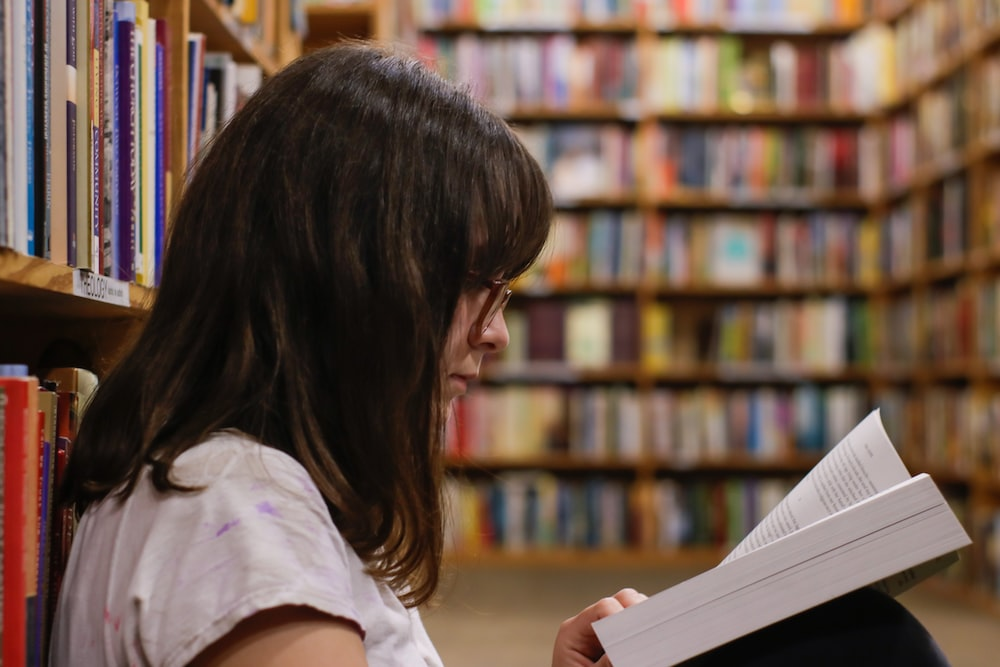
\includegraphics[width=\textwidth]{./imgs/img1.jpg}
%\caption{Fonte: https://unsplash.com/pt-br/fotografias/kcT-7cirBEw. Acesso 20/02/2023.}

É importante destacarmos também a presença de informações implícitas em
um texto, ou seja, informações que podem ser obtidas por meio da leitura
ainda que não sejam citadas explicitamente. Nesse texto, embora isto
não seja afirmado, é possível chegarmos à conclusão de que a cultura é
um aspecto muito importante de uma nação, pois permite que associemos
características específicas a um povo.

Um texto também proporciona ao leitor o aprendizado da língua. A partir
desse trecho, conhecemos palavras como “frevo” e
“moqueca”, que nomeiam importantes aspectos da cultura brasileira.

Por fim, um texto também permite que o leitor aprenda mais sobre a
estrutura das palavras. O termo “brasileira”, por exemplo, indica algo ou alguém proveniente do Brasil. Dessa forma, chegamos
à conclusão de que uma terminação como “-eiro” (que, no texto, aparece na forma feminina “-eira”) pode ser utilizada
quando necessitamos construir uma relação de pertencimento.}

\pagebreak

\colorsec{Atividades}

\num{1}  Ao lermos um texto pela primeira vez, qual aspecto devemos identificar imediatamente?

\reduline{Devemos identificar o tema trabalhado no texto.\hfill}
\linhas{1}

\num{2} Leia o trecho a seguir e identifique o tema discutido.

\begin{figure}[htpb!]
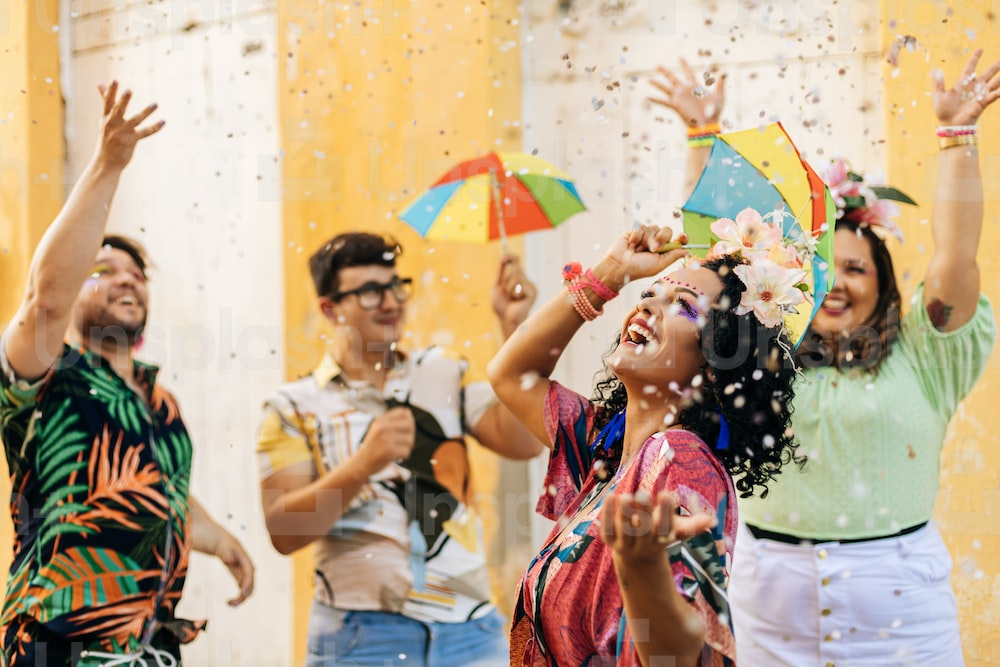
\includegraphics[width=.5\textwidth]{./imgs/img2.jpg}
%\caption{Fonte: https://unsplash.com/pt-br/fotografias/soH7UcycvKA. Acesso em: 20/02/2023.}
\end{figure}

\begin{quote}
O Carnaval brasileiro é uma das festas mais animadas e coloridas do
mundo. Celebrado anualmente, geralmente em fevereiro ou março, é um
momento de grande festa.
\fonte{Texto escrito para este material.}
\end{quote}


\reduline{O texto trata da comemoração do Carnaval no Brasil.\hfill}
\linhas{1}

\num{3} De acordo com o texto, quando o Carnaval é comemorado no Brasil?

\reduline{O Carnaval é comemorado geralmente em fevereiro ou março.\hfill}

\num{4} Assinale V para o que for verdadeiro e F para o que for falso.

\begin{boxlist}
\boxitem{F} Não podemos obter informações específicas em um texto.

\boxitem{V} Podemos aprender novas palavras por meio da leitura de um texto.

\boxitem{F} Não é importante conhecermos o tema de um texto.

\boxitem{V} É possível deduzirmos ou inferirmos informações a partir de um texto.
\end{boxlist}

Leia o texto a seguir e responda às questões de 5 a 7.

\begin{quote}
Machado de Assis foi um dos maiores escritores da literatura
brasileira. Ele nasceu no Rio de Janeiro, em 1839, e viveu em uma época
de grandes transformações no país, como a transição da monarquia para a
república e o fim da escravidão.
\fonte{Texto escrito para este material.}
\end{quote}

\num{5} Encontre no texto o ano e a cidade de nascimento do escritor Machado de Assis.

\reduline{Machado de Assis nasceu em 1839 no Rio de Janeiro.\hfill}
\linhas{1}

\num{6} De acordo com o texto, quais transformações importantes ocorreram na época de Machado de Assis?

\reduline{Machado de Assis foi contemporâneo à transição da monarquia para a
república e ao fim da escravidão.\hfill}
\linhas{1}

\num{7} Em “escritores”, encontramos a terminação “-tor”, que forma muitas palavras em língua portuguesa. Usando essa terminação, forme novas palavras relacionadas a estas:

\begin{escolha}
\item Agricultura: \reduline{agricultor.\hfill}

\item Pintura: \reduline{pintor.\hfill}

\item Canto: \reduline{cantor.\hfill}

\item Construção: \reduline{construtor.\hfill}
\end{escolha}

\num{8} Leia o texto a seguir e assinale V para o que for verdadeiro e F para o que for falso.

\begin{quote}
Luciana andava tranquilamente pela rua quando se lembrou de algo muito
importante: precisava comprar ração de gato! Estacionou, então, na
garagem de uma loja de animais e procurou a marca favorita de comida de
Lili.
\fonte{Texto escrito para este material.}
\end{quote}

\begin{boxlist}
\boxitem{V} É possível concluir que Luciana deve ter uma gata.

\boxitem{F} Luciana andava a pé pela rua quando parou para comprar ração de gato.

\boxitem{V} Lili é o nome da gata que aparece mencionada no texto.
\end{boxlist}

\coment{O aluno deve ser capaz de identificar informações implícitas no texto.}

Leia o texto a seguir e responda às questões 9 e 10.

\begin{quote}
A bossa nova é um dos movimentos musicais mais importantes do Brasil e
um dos mais reconhecidos internacionalmente. Ela surgiu na década de
1950, no Rio de Janeiro, e foi influenciada por outras formas de arte,
incluindo o jazz, o samba e a poesia.
\fonte{Texto escrito para este material.}
\end{quote}

\num{9} Encontre, no texto, fatores que influenciaram o surgimento da bossa nova.

\reduline{A bossa nova foi influenciada por formas de arte como o jazz, o samba e a poesia.\hfill}
\linhas{2}


\num{10} Como a terminação “-mente”, em “internacionalmente”, pode ser explicada com relação ao sentido que ela acrescenta à palavra primitiva?

\reduline{A terminação “-mente” é um sufixo de formação de advérbios, como os de modo, que é o caso de “internacionalmente”. Pode-se explicar a palavra derivada com a expressão “de modo internacional”.\hfill}
\linhas{2}


\colorsec{Treino}

\num{1} Leia o texto.\medskip

\begin{minipage}{.5\textwidth}
\begin{quote}
\textbf{Asteroide de mais de 1 km vai passar “próximo” da Terra nesta
quarta: entenda classificação da Nasa}

Um asteroide com cerca de \textbf{1,2 km} de diâmetro vai passar
“relativamente perto” da Terra {[}...{]}. Mas
isso não é motivo para alarde.

O chamado 199145 (2005 YY128) não representa nenhuma ameaça para nós
porque, segundo a Nasa, o
objeto passará a cerca de 12 vezes a distância média entre a Terra e a
Lua, a 4,5 milhões de quilômetros.

{[}...{]}.
\end{quote}
\end{minipage}\hspace{.2cm}
\begin{minipage}{.5\textwidth}
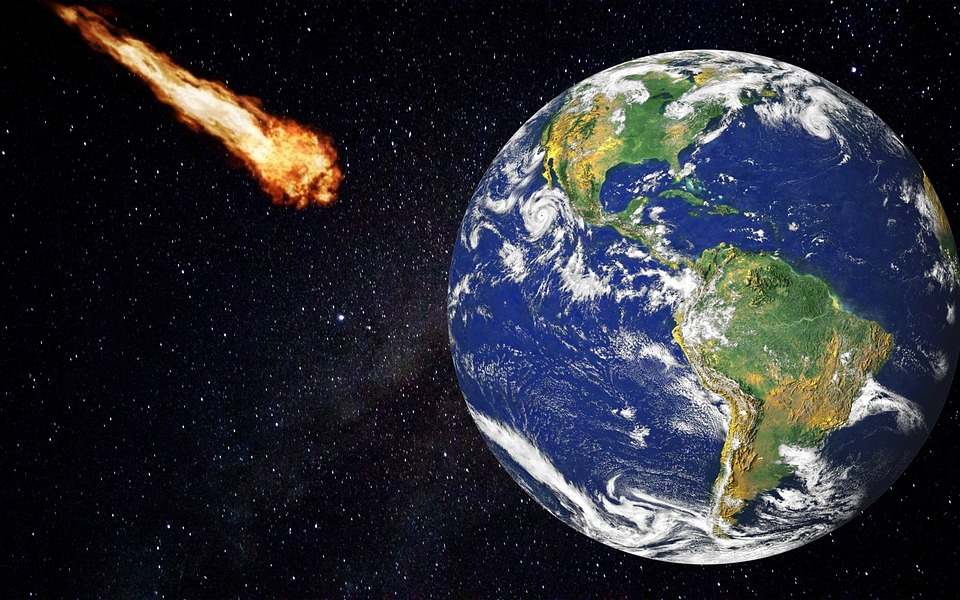
\includegraphics[width=\textwidth]{./imgs/img3.jpg}
%\caption{Fonte: https://pixabay.com/pt/photos/aster\%c3\%b3ide-cometa-meteorito-3628185/. Acesso em 20/02/2023.}
\end{minipage}

\fonte{Roberto Peixoto. Asteroide de mais de 1 km vai passar “próximo” da Terra nesta quarta: entenda classificação da Nasa. G1. Disponível em: \emph{https://g1.globo.com/ciencia/noticia/2023/02/15/asteroide-de-mais-de-1-km-vai-passar-proximo-da-terra-nesta-quarta-15-entenda-classificacao-da-nasa.ghtml}. Acesso em: 20 fev. 2023.}


Assinale o que se pode afirmar de acordo com o texto.

\begin{escolha}
\item A passagem do asteroide será perigosa para a Lua.

\item Os habitantes do planeta Terra devem ficar muito preocupados com a
aproximação do asteroide.

\item A aproximação do asteroide não representa perigo para o planeta
Terra.

\item O asteroide possui uma extensão inferior a 1 km.
\end{escolha}

\coment{SAEB: Localizar informação explícita.
BNCC: EF15LP03 -- Localizar informações explícitas em textos.}

\num{2} Leia o texto.

\begin{quote}
\textbf{Múmia extraordinariamente conservada}

Escavando túmulos na antiga necrópole de Saqqara, no Egito, arqueólogos descobriram a múmia de um homem chamado Hekashepes. Ele deve ter vivido por volta do ano 2300 a.C.

O que espantou positivamente os estudiososo é que, pensando no período da mumificação, os restos mumificados foram encontrados extraordinariamente bem conversados, dentro de um sarcófago de calcário.

\fonte{Fonte de pesquisa: Maiken Mosleth King. Arqueólogos descobrem múmia de mais de 4 mil anos coberta em ouro. BBC. Disponível em: \emph{https://www.bbc.com/portuguese/articles/cq5gge11dldo}. Acesso em:: 20 fev. 2023.}
\end{quote}

O fato de a múmia estar extraordinariamente bem preservada para o período
indica que os arqueólogos

\begin{escolha}
\item não costumam encontrar múmias bem preservadas.

\item sempre encontram múmias bem preservadas.

\item pela primeira vez encontraram uma múmia.

\item não consideram a descoberta relevante.
\end{escolha}

\coment{SAEB: Inferir informações implícitas em textos.
BNCC: EF35LP04 -- Inferir informações implícitas nos textos lidos.}

\num{3} Leia o texto.

\begin{quote}
\textbf{Asteroide entra na Terra e causa explosão de luz na Europa}

Um asteroide entrou na atmosfera da Terra por volta das 4h da manhã
(cerca de meia-noite, no horário de Brasília) no norte da França. O
objeto, ao se chocar com a atmosfera terrestre, causou um clarão.

O efeito também pôde ser visto em partes do Reino Unido. A agência de
notícias Reuters reportou imagens da luminosidade na cidade inglesa de
Brighton, localizada na beira do Canal da Mancha, que separa a
Inglaterra da França.

{[}...{]}.

\fonte{Folha de S.Paulo. Asteroide entra na Terra e causa explosão de luz na Europa. Disponível em: \emph{www1.folha.uol.com.br\%2Fciencia\%2F2023\%2F02\%2Fasteroide-entra-na-terra-e-causa-explosao-de-luz-na-europa.shtml}. Acesso em:: 20 fev. 2023.}
\end{quote}

\pagebreak
Esse texto trata:

\begin{escolha}
\item dos danos causados pelo impacto de um asteroide.

\item do aumento do número de objetos espaciais que se chocam contra a Terra.

\item da eficiência da agência de notícias Reuters.

\item do impacto de um asteroide na Terra.
\end{escolha}

\coment{SAEB: Identificar a ideia central do texto.
BNCC: EF35LP03 -- Identificar a ideia central do texto, demonstrando compreensão
global.}

\chapter{Narração e drama}
\markboth{Módulo 2}{}

\colorsec{Habilidades do SAEB}

\begin{itemize}
\item Reconhecer diferentes gêneros textuais.

\item Identificar elementos constitutivos de textos narrativos.

\item Identificar as marcas de organização de textos dramáticos.

\item Analisar os efeitos de sentido de verbos de enunciação.
\end{itemize}

\conteudo{Existem diversas maneiras de nos expressarmos textualmente. Podemos, por
exemplo, escrever uma matéria jornalística para informar o público a
respeito de temas importantes para a sociedade. Podemos, ainda, escrever
narrativas e peças de teatro com aprendizados necessários para o
desenvolvimento do ser humano.

\begin{wrapfigure}{l}{.5\textwidth}
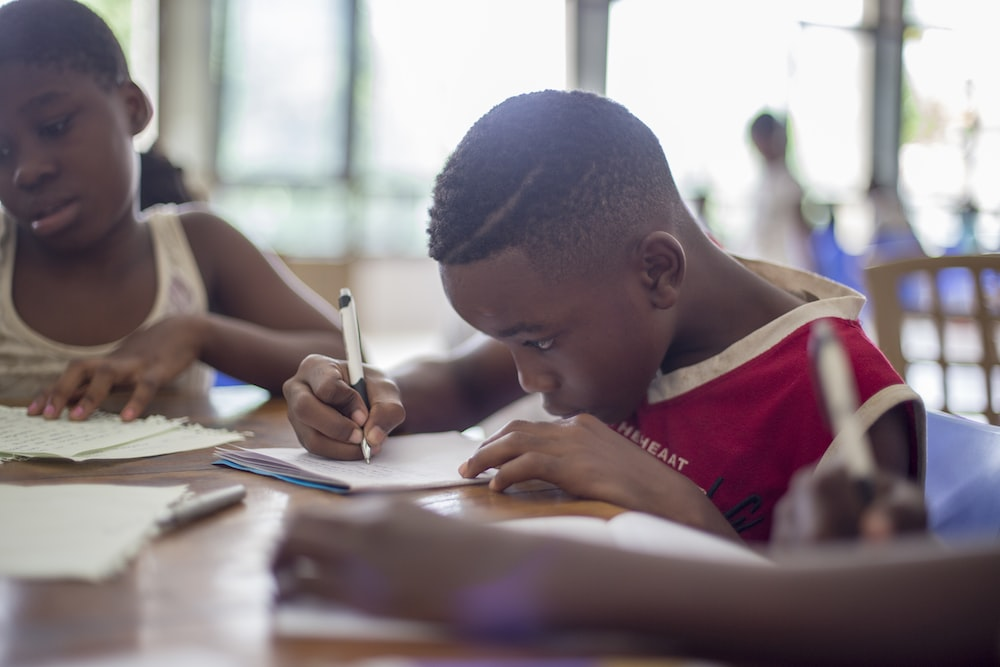
\includegraphics[width=.5\textwidth]{./imgs/img4.jpg}
%\caption{Fonte: https://unsplash.com/pt-br/fotografias/O5EMzfdxedg. Acesso em: 21 fev. 2023.}
\end{wrapfigure}

É importante reconhecermos os diferentes tipos de textos que encontramos
em nosso dia a dia. Para tanto, devemos localizar as características
específicas de cada forma de expressão. Comecemos pela narrativa. O
principal traço de um texto desse tipo é o desenvolvimento de uma hisstória com personagens, espaço e tempo por meio da intermediação de um narrador.

Para compreendermos algumas dessas características, tomemos como exemplo
o início de uma famosa história infantil.

\begin{quote}
\textbf{Chapeuzinho Vermelho}

Era uma vez uma menina chamada Chapeuzinho Vermelho. Ela morava em uma
casa na floresta com sua mãe.

Certo dia, a mãe de Chapeuzinho lhe fez um pedido:

--- Minha filha, leve esses doces para sua avó! Ela está doente!

A alegre menina respondeu:

--- Mas é claro, mamãe!

Chapeuzinho Vermelho colocou sua capa vermelha e saiu em sua jornada.

Enquanto caminhava pela floresta, Chapeuzinho Vermelho encontrou um lobo
malvado, que perguntou para onde ela estava indo. Chapeuzinho Vermelho
respondeu que estava indo visitar sua avó e mostrou-lhe o caminho.

{[}...{]}.
\end{quote}
}

\conteudo{A presença de personagens é uma característica que podemos destacar
nesse trecho. Nesse caso específico, encontramos Chapeuzinho Vermelho,
sua mãe e o lobo. Um texto narrativo deverá sempre apresentar
personagens que, em certo sentido, conduzem a história sendo contada,
mas são apresentados por um narrador. Quando aparece, as falas são
introduzidas por um travessão, tal como pode ser observado no trecho.

\marginnote{Os alunos serão apresentados a ao texto narrativos e aos
textos dramáticos. A partir da leitura dos trechos apresentados,
você deve destacar as características específicas desses textos,
fazendo com que a turma seja capaz de reconhecê-los prontamente.\\
Habilidades da BNCC: EF05LP09, EF05LP10, EF05LP15, EF05LP22, EF35LP24,
EF35LP26 e EF35LP29.}

Os diálogos normalmente são introduzidos por meio de verbos de
enunciação, isto é, verbos que indicam alguma ação relacionada à fala.
Nesse trecho de “Chapeuzinho Vermelho”, encontramos o verbo “responder”
antes da resposta de Chapeuzinho. Outros verbos comuns são: “falar”,
“dizer”, “afirmar”, “exclamar”, por exemplo.

\begin{wrapfigure}{l}{.3\textwidth}

\includegraphics[width=.3\textwidth]{./imgs/img5.png}
%\caption{Fonte: https://pixabay.com/pt/vectors/chapeuzinho-vermelho-garota-corrida-156953/. Acesso em: 21 fev. 2023.}
\end{wrapfigure}

Por fim, é necessário percebermos também como uma narrativa sempre
apresenta um narrador, ou seja, uma voz que conta a história. No trecho
reproduzido, é possível percebermos como a narrativa é apresentada
aos leitores por meio de uma voz que parece conhecer todos os fatos a
serem transmitidos.

Semelhante, em alguns aspectos, a uma narrativa, mas diferente em outros, existe o texto dramático, que é aquele escrito para ser encenado. Talvez, você já tenha asssistido a uma peça de teatro no palco. Para aprenderem suas falas
e apresentarem a história em cima do palco, os atores devem ler o texto
dramático, que consiste em uma sequência de diálogos
entre personagens.

Tomemos como exemplo uma história de Chapeuzinho
Vermelho em formato de texto dramático.

\begin{quote}
Chapeuzinho Vermelho (aproximando-se da cama): Para que esses olhos
tão grandes, vovozinha?

Lobo: São para te enxergar melhor!

Chapeuzinho Vermelho: E para que essas orelhas tão grandes, vovozinha?

Lobo: São para te escutar melhor!
\end{quote}

Percebemos como um texto dramático apresenta os diálogos a serem
decorados pelos atores de uma peça. Ao invés de um travessão, as falas são introduzidas pelos nomes dos personagens envolvidos.

Podemos, ainda, notar a presença da descrição de uma ação a ser realizada, que,
no caso, é a aproximação de Chapeuzinho à cama de sua avó. Essas indicações marcam a ação dos atores no palco. Assim,
constatamos como, em um texto dramático, o desenrolar da história é
apresentado diretamente ao leitor, sem a presença de um narrador.}

\colorsec{Atividades}

\num{1} Como denominamos a voz que apresenta a narrativa aos leitores?

\reduline{O narrador é que apresenta os fatos de uma história ao leitor.\hfill}

\num{2} Como chamamos os indivíduos que participam de uma narrativa e de um
texto dramático?

\reduline{Tanto o texto narrativo quanto o texto dramático contam com a presença de personagens.\hfill}

\num{3} Em um texto dramático, como a história é apresentada ao leitor?

\reduline{Um texto dramático apresenta o diálogo como sua estrutura básica.\hfill}

\num{4} Assinale V para o que for verdadeiro e F para o que for falso.

\begin{boxlist}
\boxitem{F} Em um texto dramático, não são descritas as ações dos personagens.

\boxitem{V} O verbo “falar” pode ser usado para introduzir um diálogo.

\boxitem{F} Um texto dramático sempre apresenta um narrador.

\boxitem{V} Diferentemente do texto dramático, o texto narrativo não é escrito para ser encenado.
\end{boxlist}

Leia o texto e responda às questões 5 e 6.

\begin{quote}
Príncipe (caminhando em direção à torre, gritando): Quem é esta bela
donzela presa no topo da torre?

Rapunzel: Sou eu: Rapunzel! A jovem dos cabelos dourados.
\fonte{Texto escrito para este material.}
\end{quote}

\num{5} Quais são os personagens envolvidos nesse texto?

\reduline{O texto apresenta os personagens Príncipe e Rapunzel.\hfill}
\linhas{1}

\num{6} Mesmo não se tratando de um texto narrativo, aparece um verbo de enunciação antecedendo a fala do Príncipe. Que verbo é esse?

\reduline{Foi utilizado o verbo “gritar”.\hfill}
\linhas{1}

\pagebreak
\num{7} Associe as colunas.

{\setlength{\columnsep}{-5cm}
\begin{multicols}{2}
(1) Texto narrativo

(2) Texto dramático

\columnbreak

({\rosa{1}}) Presença de um narrador.

({\rosa{2}}) Diálogos introduzidos pelos nomes dos personagens.

({\rosa{2}}) Ação apresentada diretamente ao leitor.

({\rosa{1}}) Diálogos introduzidos por um travessão.
\end{multicols}
}

\num{8} Qual é a diferença fundamental entre um texto narrativo e um texto dramático?

\reduline{Em um texto narrativo, a história é contada pelo narrador. Já em um texto
dramático, a ação acontece a partir dos diálogos entre os personagens.\hfill}
\linhas{1}

Leia o texto e responda às questões 9 e 10.\medskip

\begin{minipage}{.5\textwidth}
\begin{quote}
Certa vez, uma lebre e uma tartaruga decidiram apostar uma corrida.

A lebre era muito rápida e estava confiante de que venceria. Ela se
deitou para tirar uma soneca enquanto a tartaruga continuava a andar.

No entanto, a tartaruga não desistiu e continuou a se mover em um ritmo
constante. Quando a lebre acordou de sua soneca, viu que a tartaruga
havia quase chegado ao final da corrida.

A lebre correu o mais rápido que pôde para tentar recuperar o atraso,
mas foi tarde demais. A tartaruga cruzou a linha de chegada antes,
vencendo a corrida.
\fonte{Texto escrito para este material.}
\end{quote}
\end{minipage}
\begin{minipage}{.5\textwidth}
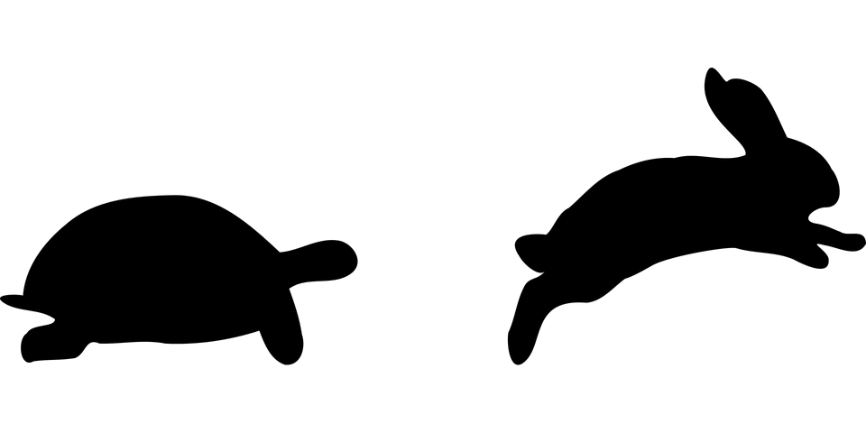
\includegraphics[width=\textwidth]{./imgs/img6.png}
%\caption{Fonte: https://pixabay.com/pt/vectors/imagens-de-palavras-do-alfabeto-1298865/. Acesso em: 21 fev. 2023.}
\end{minipage}

\num{9} Esse texto é uma narrativa ou um drama? Justifique sua resposta.

\reduline{Trata-se de uma narrativa, pois a ação é apresentada por um narrador, e
não por meio de diálogos.\hfill}
\linhas{1}

\num{10} Quais são os personagens envolvidos no texto?

\reduline{As personagens são a Lebre e a Tartaruga.\hfill}

\pagebreak

\colorsec{Treino}

\num{1} Leia o texto.

\begin{quote}
{[}...{]}

--- Errou! --- Interrompeu Camilo, rindo.

--- Não diga isso, Camilo. Se você soubesse como eu tenho andado, por
sua causa. Você sabe; já lhe disse. Não ria de mim, não ria...

Camilo pegou-lhe nas mãos e olhou para ela sério e fixo. Jurou que lhe
queria muito, que os seus sustos pareciam de criança.

{[}...{]}

\fonte{Joaquim Maria Machado de Assis. A Cartomante.
Disponível em: /emph{https://machado.mec.gov.br/obra-completa-lista/item/download/65\_2b8fb9ad43aa37653a58bc2bd56e33aa}. Acesso em:: 21 fev. 2023.}
\end{quote}

Os diálogos desse texto narrativo são introduzidos por meio de

\begin{minipage}{.5\textwidth}
\begin{escolha}
\item aspas.

\item travessões.

\item vírgulas.

\item pontos finais.
\end{escolha}
\end{minipage}
\sidetext{SAEB: Identificar elementos constitutivos de textos narrativos.
BNCC: EF35LP26 -- Ler e compreender, com certa autonomia, narrativas ficcionais
que apresentem cenários e personagens, observando os elementos da
estrutura narrativa: enredo, tempo, espaço, personagens, narrador e a
construção do discurso indireto e discurso direto.}

\num{2} Leia o texto.

\begin{quote}
{[}...{]}

O estrangeiro disse:

--- Sou dos guerreiros brancos, que levantaram a taba nas margens do
Jaguaribe, perto do mar, onde habitam os pitiguaras, inimigos de tua
nação. Meu nome é Martim, que na tua língua diz como filho de guerreiro;
meu sangue, o do grande povo que primeiro viu as terras de tua pátria.

{[}...{]}.

\fonte{José de Alencar. Iracema. Disponível em: \emph{http://objdigital.bn.br/Acervo\_Digital/Livros\_eletronicos/iracema.pdf}. Acesso em:: 21 fev. 2023.}
\end{quote}

O verbo de enunciação utilizado para introduzir a fala do personagem indica que ele

\begin{escolha}
\item pronunciou a fala sem nenhuma forma de expressão específica.

\item gritou aquilo que pretendia pronunciar para seu interlocutor.

\item susurrou para seu interlocutor, mesmo correndo o risco de não ser ouvido.

\item pronunciou a fala indicada nas costas de seu interlocutor.
\end{escolha}

\coment{SAEB: Analisar os efeitos de sentido de verbos de enunciação.
BNCC: EF05LP09 -- Ler e compreender, com autonomia, textos instrucionais de
regras de jogo, dentre outros gêneros do campo da vida cotidiana, de
acordo com as convenções do gênero e considerando a situação
comunicativa e a finalidade do texto.}

\num{3} Leia o texto.

\begin{quote}
{[}...{]}

BARÃO (à porta) --- Perdão, minha senhora; eu trazia um livro há
pouco...

D. HELENA (com o livro na mão) --- Será este?

BARÃO (caminhando para ela) --- Justamente.

D. HELENA --- Escrito em sueco, penso eu...

BARÃO --- Em sueco.

{[}...{]}.
\end{quote}

\fonte{Joaquim Maria Machado de Assis. Lição de Botânica. Disponível em: \emph{https://machado.mec.gov.br/obra-completa-lista/item/download/65\_2b8fb9ad43aa37653a58bc2bd56e33aa}. Acesso em:: 21 fev. 2023.}

A informação “caminhando para ela”, entre parênteses, indica

\begin{minipage}{.5\textwidth}
\begin{escolha}
\item uma parte do narrador.

\item uma marcação do cenário.

\item o início de uma fala.

\item uma ação do personagem.
\end{escolha}
\end{minipage}
\sidetext{SAEB: Identificar as marcas de organização de textos dramáticos.
BNCC: EF35LP24 -- Identificar funções do texto dramático (escrito para ser
encenado) e sua organização por meio de diálogos entre personagens e
marcadores das falas das personagens e de cena.}

\chapter{O gênero notícia}
\markboth{Módulo 3}{}

\coment{Neste módulo, estudaremos o gênero textual notícia. Você deve
examinar os traços associados a esse gênero com os alunos,
destacando sua natureza informativa. Também exploraremos algumas regras
de pontuação da língua portuguesa a partir das notícias apresentadas.\\
Habilidades da BNCC: EF35LP16 e EF05LP14.}

\colorsec{Habilidades do SAEB}

\begin{itemize}
\item Analisar elementos constitutivos de gêneros textuais diversos.

\item Reconhecer os usos da pontuação.

\item Analisar os efeitos de sentido decorrentes do uso da pontuação.
\end{itemize}

\conteudo{Cotidianamente, entramos em contato com muitos gêneros textuais
diferentes. Cada texto possui características próprias
relacionadas ao assunto explorado e ao público que pretende atingir.
Devemos conhecer esses traços para identificarmos as muitas formas de
nos expressarmos. Para exemplificarmos esse processo, tomemos como
exemplo um gênero muito comum em nosso dia a dia.

\begin{wrapfigure}{l}{.5\textwidth}
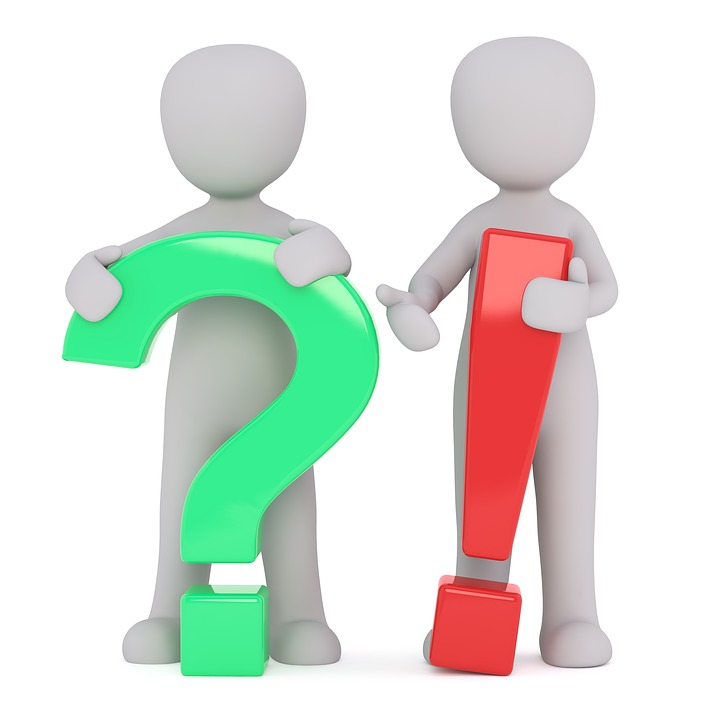
\includegraphics[width=.5\textwidth]{./imgs/img7.jpg}
%\caption{Fonte: https://pixabay.com/pt/illustrations/ponto-de-interroga\%c3\%a7\%c3\%a3o-pergunta-ajuda-2314115/. Acesso em: 21 fev. 2023.}
\end{wrapfigure}

Uma excelente maneira de nos mantermos informados a respeito do mundo se
dá por meio da leitura de notícias veiculadas, por exemplo, em jornais, revistas ou sites de
internet. De modo geral, esse gênero trata de fatos recentes de alguma
relevância para a sociedade. Ao consumirmos uma notícia, devemos
nos atentar para algumas de suas características principais a fim de
absorvermos todo o seu conteúdo.}

\conteudo{Para identificar os traços estilísticos de uma notícia, leia o trecho
a seguir.

\begin{quote}
\textbf{Brasileiros estão entre os que mais receberam vistos norte-americanos}
\textit{País ficou atrás apenas de México e China em 2022}

Pesquisa da AG Immigration – escritório de advocacia imigratória com sede em Washington – mostra que os brasileiros ocuparam o terceiro lugar no ranking dos que mais receberam vistos norte-americanos em 2022. Ao todo, foram 815.842 emissões de 80 tipos diferentes de permissões, alta de 618,8\% em relação ao registrado no ano anterior (113.505). Em comparação com 2018 (640.998), nos níveis de antes da pandemia de covid-19, o aumento foi de 26,4\%.

O Brasil ficou atrás apenas do México (1,9 milhão) e da China (1 milhão), e bem à frente da Argentina, quarta colocada, com 259 mil vistos recebidos.

O levantamento foi feito com base em dados oficiais do Departamento de Estado norte-americano, de janeiro a dezembro de 2022. {[}...{]}.

\fonte{Ana Cristina Campos. Brasileiros estão entre os que mais receberam vistos norte-americanos. Agência Brasil. Disponível em: \emph{https://agenciabrasil.ebc.com.br/internacional/noticia/2023-03/brasileiros-estao-entre-os-que-mais-receberam-vistos-norte-americanos}. Acesso em:: 23 mar. 2023.}
\end{quote}

Em primeiro lugar, é possível identificar o título da notícia: “Brasileiros estão entre os que mais receberam vistos norte-americanos”. Nos locais em que costumam ser veiculadas as notícias, o título geralmente ocupa o
centro da página e apresenta uma fonte maior, em destaque. Dessa forma,
o leitor será capaz de compreender o assunto da notícia.

Logo em seguida, logo abaixo do título, aparece o subtítulo, que amplia as informações do título e, no caso dessa notícia, destaca um ponto relevante presente no corpo do texto.

Então, inicia-se o texto da notícia em si. O primeiro parágrafo de uma notícia, chamado de \textbf{lide}, condensa todas as informações a serem pormenorizadas no corpo do texto, que se inicia no próximo parágrafo.

Algo que devemos ter mente ao lermos o texto de uma notícia é a natureza
expressiva utilizada por seu autor. É possível transmitir informações
aos leitores, não somente por meio de palavras, mas também sinais de
pontuação. No texto acima, por exemplo, encontramos o uso recorrente de
vírgulas e pontos finais, por exemplo. Enquanto as vírgulas são usadas
para separar diferentes frases e organizar os elementos que as compõem, o
ponto final marca o final de um enunciado.}

\pagebreak
\colorsec{Atividades}

\num{1} Como podemos diferenciar os diversos gêneros textuais que
encontramos todos os dias?

\reduline{Devemos conhecer as características específicas de cada gênero textual, bem como o meio em que circulam e o objetivo a que se propõem.\hfill}
\linhas{1}


\num{2} Em geral, do que trata uma notícia?

\reduline{Uma notícia trata de fatos recentes relevantes para a sociedade.\hfill}
\linhas{1}

\num{3} Como se chama a parte de uma notícia que surge ao centro da página
em uma fonte maior?

\reduline{Trata-se do título da notícia, que também pode ser denominado de manchete.\hfill}

\num{4} Qual é a função do texto inserido logo após o título de uma notícia? Como ele se chama?

\reduline{Trata-se do subtítulo, que cumpre funções como ampliar as informações do título, resumir o conteúdo da notícia ao leitor ou, ainda, destacar um ponto importante do corpo do texto.\hfill}
\linhas{2}

\num{5} Pensando no fluxo de leitura de notícias, tente refletir sobre a importância do lide e explique por que o primeiro parágrafo pode ser importante nesse sentido.

\reduline{Alguns leitores podem se interessar por ler muitas notícias seguidamente, e,
nesse sentido, a condensação das informações importantes sobre um fato em um mesmo
parágrafo (o primeiro) pode ajudar o leitor a terminar a leitura de forma mais ágil,
de modo que se parta para os próximos parágrafos caso sinta necessidade de ter detalhes
sobre um aspecto.\hfill}
\linhas{2}

\num{6} Assinale V para o que for verdadeiro e F para o que for falso.

\begin{boxlist}
\boxitem{F} Uma notícia não costuma apresentar um título.

\boxitem{F} O principal assunto da notícia não costuma aparecer em seu título.

\boxitem{V} O principal intuito de uma notícia é informar o leitor.

\boxitem{V} Uma notícia deve expor ao leitor diferentes informações sobre
determinado tema.
\end{boxlist}\pagebreak

\num{7} Associe as colunas.

\begin{multicols}{2}
(1) Ponto final.\medskip

(2) Vírgula.\medskip

(3) Ponto de interrogação.\medskip

(4) Ponto de exclamação.

\columnbreak

({\rosa{3}}) Sinal de pontuação que é empregado

para indicar uma pergunta.\medskip

({\rosa{2}}) Sinal de pontuação que é utilizado

para separar frases.\medskip

({\rosa{1}}) Sinal de pontuação que é colocado ao

final das frases.\medskip

({\rosa{4}}) Sinal de pontuação que é usado para

destacar informações.
\end{multicols}


Leia o texto a seguir e responda às questões de 8 a 10.

\begin{quote}
\textbf{Quaoar, espécie de primo de Platão, tem anel}\\
\textit{A descoberta desafia a principal teoria de formação de anéis}

Quaoar é um dos grandes objetos de grande porte que orbita além de Netuno.
Recentemente, pesquisadores de vários países descobriram que Quaoar tem um
anel, e isso sugere que essa estrutura deve ser bem mais comum do que se
pensava até então. Com isso, a compreensão sobre a formação de um anel
foi colocada em xeque.

\fonte{Fonte de pesquisa: Salvador Nogueira. Brasileiros descobrem anel em Quaoar,
“primo” de Plutão. Folha de S.Paulo. Disponível em: \emph{https://www1.folha.uol.com.br/ciencia/2023/02/brasileiros-descobrem-anel-em-quaoar-primo-de-plutao.shtml}. Acesso em:: 23 mar. 2023.}
\end{quote}

\num{8} Com base nesse primeiro parágrafo da notícia, depreenda qual é o assunto tratado.

\reduline{A notícia trata da descoberta de um anel ao redor de um corpo celeste longínquo chamado Quaoar.\hfill}
\linhas{2}


\num{9} O título da notícia é totalmente claro, para qualquer leitor, com relação ao assunto tratado?

\reduline{Pode-se perceber que, sobretudo para um leitor leigo, o assunto da notícia só fica totalmente claro no primeiro parágrafo da notícia.\hfill}
\linhas{1}


\num{10} Quais são os sinais de pontuação encontrados no texto e quais são
suas funções?

\reduline{O texto apresenta vírgulas e pontos finais. Esses sinais são utilizados
para separar frases e indicar o fim de uma sentença, respectivamente.\hfill}
\linhas{1}


\colorsec{Treino}

\num{1} Leia o texto.

\begin{figure}[htpb!]
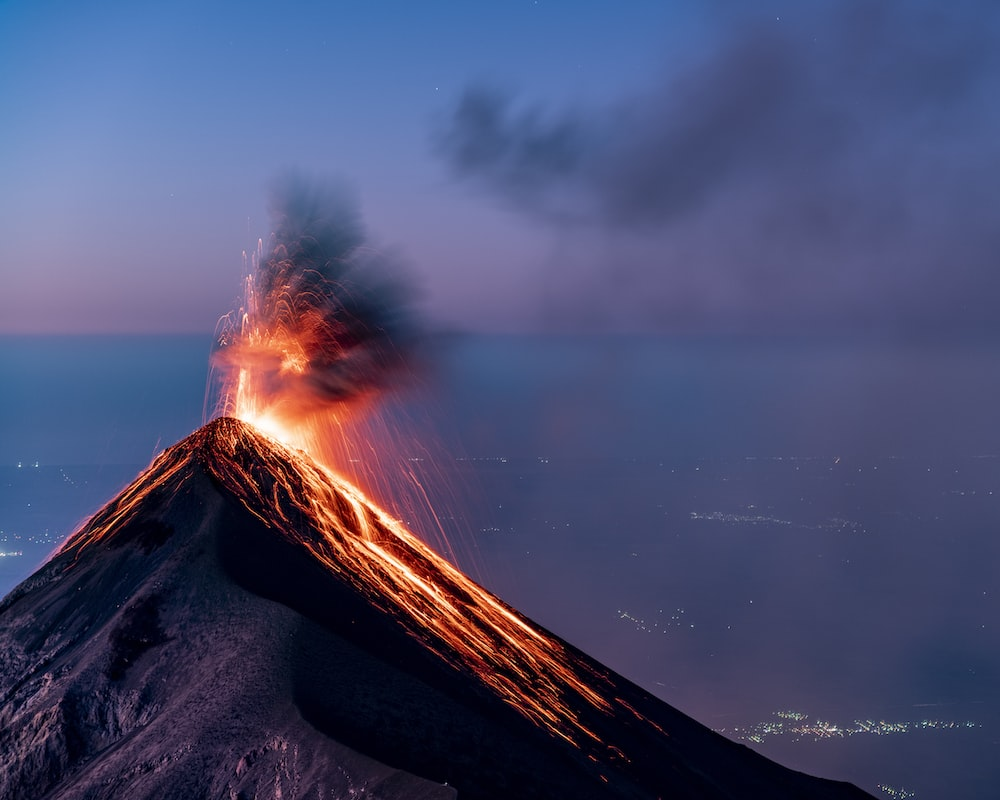
\includegraphics[width=.5\textwidth]{./imgs/img9.jpg}
%\caption{Fonte: https://unsplash.com/pt-br/fotografias/tLxGw\_ITs7k. Acesso em 21/03/2022.}
\end{figure}

\begin{quote}
\textbf{Maior vulcão ativo do mundo entra em erupção no Havaí}

O maior vulcão ativo do mundo, que fica no Havaí, entrou em erupção pela primeira vez em 40 anos. Localizado no Parque Nacional dos Vulcões, o Mauna Loa cobre metade da Ilha do país e se eleva há mais de quatro mil metros do nível do mar.

O fluxo de lava está localizado principalmente no cume, mas os moradores foram colocados em alerta. No entanto, nenhuma ordem para deixar o local foi emitida, pois as autoridades acham improvável que as áreas povoadas sejam afetadas nesta fase. Um aviso de queda de cinzas chegou a ser emitido, mas já foi suspenso.

De acordo com o Serviço Geológico dos Estados Unidos, o Mauna Loa entrou em erupção 33 vezes desde 1843. A última foi em 1984, quando as lavas chegaram a atingir a cidade de Hilo, a mais populosa da ilha.

\fonte{Repórter Brasil Tarde. Maior vulcão ativo do mundo entra em erupção no Havaí. Disponível em: \emph{https://tvbrasil.ebc.com.br/reporter-brasil-tarde/2022/11/maior-vulcao-ativo-do-mundo-entra-em-erupcao-no-havai}. Acesso em:: 23 mar. 2023.}
\end{quote}

O uso do presente do indicativo (“entra”) no título do texto

\begin{escolha}
\item aproxima do leitor o fato ocorrido e noticiado.

\item cria uma distância temporal entre o fato e a notícia.

\item estabelece que o fato noticiado ainda está para acontecer.

\item demonstra que o fato ocorre no momento da publicação da notícia.
\end{escolha}

\coment{SAEB: Analisar elementos constitutivos de gêneros textuais diversos.
BNCC: EF35LP16 -- Identificar e reproduzir, em notícias, manchetes, lides
e corpo de notícias simples para público infantil e cartas de reclamação
(revista infantil), digitais ou impressos, a formatação e diagramação
específica de cada um desses gêneros, inclusive em suas versões orais.}



\num{2} Leia o texto.

\begin{quote}
\textbf{Novo mapa da Via Láctea revela mais de 3,3 bilhões de objetos e
detalhes inéditos da nossa galáxia}
\textit{Catálogo pode ser considerado o maior do tipo até então}

Uma nova imagem com detalhes sem precedentes da Via Láctea foi lançada
nesta quinta-feira (19) para marcar a segunda fase de uma das maiores
pesquisas de rastreio da galáxia da qual o nosso Sistema Solar faz parte
{[}...{]}.

Como resultado do levantamento gigantesco, que levou dois anos para ser
concluído, cerca de 3,32 bilhões de objetos foram identificados, o que
pode ser considerado o maior catálogo do tipo até então.

{[}...{]}
\fonte{Roberto Peixoto. Novo mapa da Via Láctea revela mais de 3,3 bilhões de objetos e detalhes inéditos da nossa galáxia. G1. Disponível em: \emph{https://g1.globo.com/ciencia/noticia/2023/01/19/novo-mapa-da-via-lactea-revela-mais-de-33-bilhoes-de-objetos-e-detalhes-ineditos-da-nossa-galaxia.ghtml}. Acesso em:: 23 mar. 2023.}
\end{quote}

Uma marca temporal presente nessa notícia revela que o fato noticiado é

\begin{minipage}{.5\textwidth}
\begin{escolha}
\item recente.

\item antigo.

\item ultrapasado.

\item futuro.
\end{escolha}
\end{minipage}
\sidetext{SAEB: Analisar elementos constitutivos de gêneros textuais diversos.
BNCC: EF35LP16 -- Identificar e reproduzir, em notícias, manchetes, lides
e corpo de notícias simples para público infantil e cartas de reclamação
(revista infantil), digitais ou impressos, a formatação e diagramação
específica de cada um desses gêneros, inclusive em suas versões orais.}


\num{3} Leia o texto.

\begin{quote}
\textbf{Mais energia do que o Sol? Cientistas devem revelar “grande
avanço científico”}

O Departamento de Energia dos Estados Unidos afirmou no domingo que
anunciará durante a semana um “grande avanço científico”, depois que
vários meios de comunicação informaram que um laboratório federal
alcançou recentemente um marco importante na pesquisa da fusão nuclear.

{[}...{]}.

\fonte{TILT. Mais energia do que o Sol? Cientistas devem revelar “grande
avanço científico”. Disponível em: \emph{https://www.uol.com.br/tilt/noticias/afp/2022/12/12/mais-energia-do-que-o-sol-cientistas-irao-revelar-grande-marco-em-fusao-nuclear.htm}. Acesso em:: 21 mar. 2023.}
\end{quote}

O ponto de interrogação é empregado no título da notícia para

\begin{minipage}{.5\textwidth}
\begin{escolha}
\item indicar uma pergunta.

\item destacar o tema a ser discutido.

\item dividir duas frases.

\item indicar o final do texto.
\end{escolha}
\end{minipage}
\sidetext{SAEB: Analisar os efeitos de sentido decorrentes do uso da pontuação.
BNCC: EF05LP04 -- Diferenciar, na leitura de textos, vírgula, ponto e
vírgula, dois-pontos e reconhecer, na leitura de textos, o efeito de
sentido que decorre do uso de reticências, aspas, parênteses.}

\chapter{Argumentação e persuasão}
\markboth{Módulo 4}{}

\colorsec{Habilidades do SAEB}

\begin{itemize}
\item Analisar o uso de recursos de persuasão em textos verbais e/ou
multimodais.

\item Analisar os efeitos de sentido de recursos multissemióticos em textos
que circulam em diferentes suportes.

\item Julgar a eficácia de argumentos em textos.
\end{itemize}

\marginnote{Os alunos serão expostos a textos argumentativos neste módulo. O
professor deverá analisar as características do gênero a fim de
demonstrar como um argumento convincente é construído. Além disso, a
partir da leitura de imagens serão também estudadas as possibilidades
multissemióticas implícitas no processo de argumentação.\\
Habilidade da BNCC: EF05LP20.}
\conteudo{No módulo anterior, estudamos o gênero notícia, que é focado
na transmissão de informações. É importante, todavia, destacarmos outras
possibilidades textuais que buscam criar efeitos diversos nos leitores.
É possível, por exemplo, encontrarmos textos que tentam convencer o
público da validade de um ponto de vista ou ação. Denominamos esse texto
de \textbf{argumentativo}.

\begin{wrapfigure}{l}{.4\textwidth}
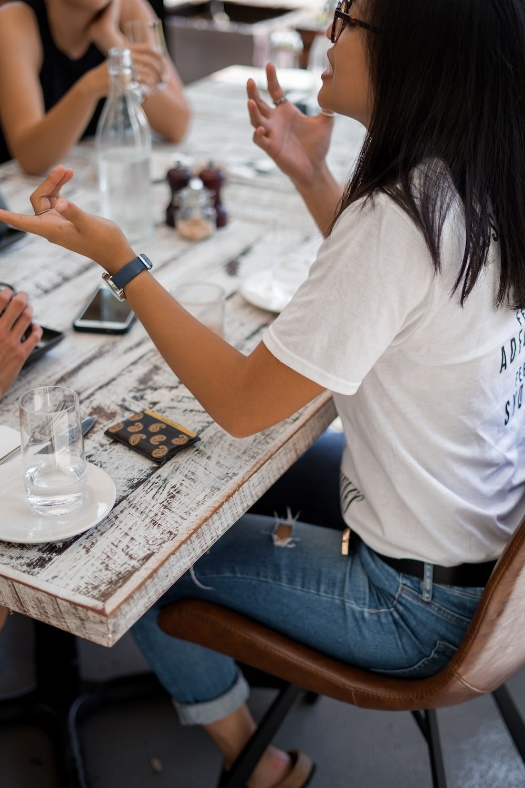
\includegraphics[width=.4\textwidth]{./imgs/img10.jpg}
%\caption{Fonte: https://unsplash.com/pt-br/fotografias/wXJViXxHP44. Acesso em 20/02/2023.}
\end{wrapfigure}

Ao analisarmos esse tipo de texto, é importante termos em mente dois aspectos
importantes: a tese sobre a qual o autor está tentando convencer os
leitores e as estratégias utilizadas para atingir esse objetivo. Leia
o texto a seguir para analisar esses aspectos.

\begin{quote}
\textbf{A Turminha está em campanha contra a dengue}

A Turminha do MPF anda preocupada com a dengue. Também não é para
menos: a Sol foi picada pelo mosquito e ficou dodói. Depois de vários
dias de repouso, tomando muito líquido, agora já está bem.

A Malu, preocupada com a amiga doente, ficou indignada com pessoas que
deixam água parada e alertou os amigos da Turminha para chamarem a
defesa civil quando souberem de algum lote vazio onde haja foco de
dengue. Na rua do Rafinha houve um surto de dengue e muitas pessoas
ficaram doentes. Ele deu dicas sobre os cuidados com as piscinas e com
objetos que acumulam água, como pneus, garrafas, tampinhas etc.
{[}...{]}.
\end{quote}

\fonte{Turminha do MPF. A Turminha está em campanha contra a dengue.
Disponível em:\emph{https://bit.ly/3nxuY74}. Acesso em: 21 fev. 2023.}
}

\conteudo{Consegue identificar o argumento construído acima? Trata-se de um texto
escrito com o intuito de expor os perigos da dengue e de convencer as
crianças da necessidade de combatermos o mosquito \textit{Aedes aegypti}. Para
isso, o autor utiliza o exemplo da garotinha Sol, que contraiu a doença
e precisou passar alguns dias de repouso até se curar. Percebe-se que, para se
criar um argumento convincente, pode ser importante exemplificar situações
relacionados ao assunto explorado.

Ao construirmos um argumento, é necessário explicarmos o que o leitor
deve fazer para atingir o objetivo exposto em nosso texto. No caso
específico do combate à dengue, foram enumeradas, nesse trecho do texto,
atitudes a serem tomadas a fim de impedir a proliferação do mosquito da
dengue -- chamar a Defesa Civil e não deixar água parada em pneus, por exemplo.
Dessa forma, podemos dizer que a argumentação depende de ações
explicadas objetivamente.

Um texto argumentativo pode também ser construído a partir de outras
formas de expressão que não a da escrita. A utilização de imagens é uma
estratégia eficiente e chamativa para fortalecer um argumento. Em um
texto sobre a dengue, é possível, por exemplo, encontrarmos um pôster
que estimule o combate ao mosquito. Veja a imagem a seguir.

\begin{wrapfigure}{l}{.4\textwidth}
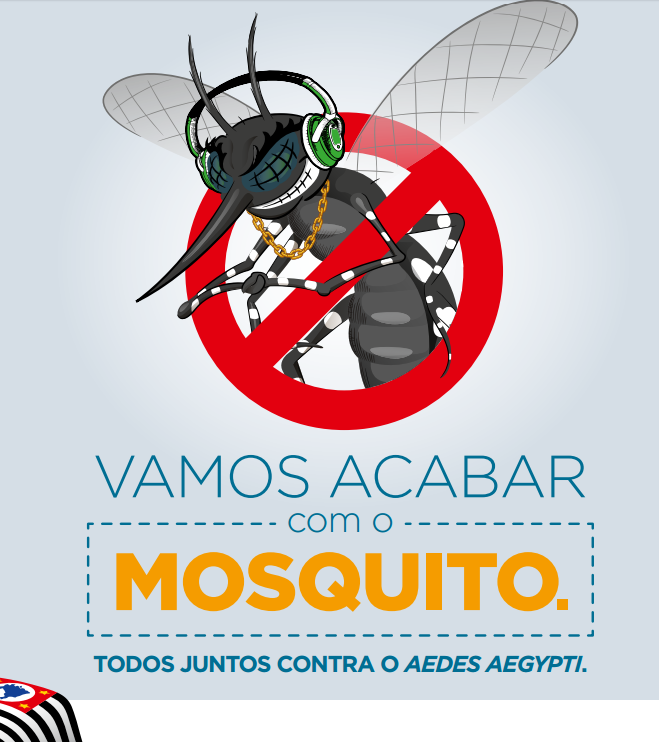
\includegraphics[width=.4\textwidth]{./imgs/img11.png}
%\caption{Fonte: https://www.saopaulo.sp.gov.br/tag/dengue/. Acesso em: 21 fev. 2023.}
\end{wrapfigure}

Com esse cartaz, é possível percebermos como um texto argumentativo pode lançar mão de
diferentes estratégias para atingir seus objetivos, até mesmo de
artifícios visuais. O desenho do mosquito dentro do
símbolo associado a proibição fortalece o argumento a ser desenvolvido.
De maneira chamativa, é salientada a necessidade de tomarmos atitudes diretas contra o
\textit{Aedes aegypti}.

Após a leitura de um texto argumentativo, o leitor poderá julgar se as
estratégias transmitidas foram eficientes, isto é, se o texto foi
convincente ou não. A eficácia de um argumento está diretamente
relacionada à qualidade de exemplos e ações apresentados. No texto de
combate à dengue, podemos dizer que o autor conseguiu desenvolver uma
ideia convincente, já que ofereceu exemplos e ações capazes de
solucionar o problema exposto.}

\pagebreak
\colorsec{Atividades}

\num{1} Como denominamos o tipo textual utilizado para tentar convencer o leitor
de algo?

\reduline{Trata-se do texto argumentativo.\hfill}

\num{2} Quais são os dois elementos principais desse tipo de texto?

\reduline{Um texto argumentativo é essencialmente constituído por tese e argumentos.\hfill}
\linhas{1}

\num{3} Assinale V para o que for verdadeiro e F para o que for falso.

\begin{boxlist}
\boxitem{F} É melhor que um texto argumentativo não cite exemplos relacionados à tese.

\boxitem{F} Um texto argumentativo não pretende convencer o leitor a respeito de
um ponto de vista.

\boxitem{V} Um texto argumentativo pode apresentar ações a serem realizadas por alguém em prol de um objetivo relacionado à tese.

\boxitem{F} Um texto argumentativo só deve ser constituído por palavras.
\end{boxlist}

\num{4} Após a leitura de um texto argumentativo, como podemos julgar os argumentos apresentados?

\reduline{Devemos verificar se os argumentos apresentados foram convincentes.\hfill}
\linhas{1}

\num{5} Pensando no cartaz sobre o mosquito \textit{Aedes aegypti}, complete a frase a seguir.

\bigskip

\noindent{}Além da escrita, um texto argumentativo pode apresentar \reduline{imagens\hfill}.

\bigskip

Leia o texto a seguir e responda às questõe de 6 a 8.

\begin{quote}
\textbf{SP contra o novo coronavírus}

{[}...{]}

\textit{Lave as mãos}

\begin{figure}[htpb!]
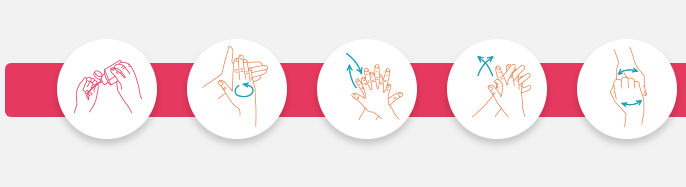
\includegraphics[width=.5\textwidth]{./imgs/img12.png}
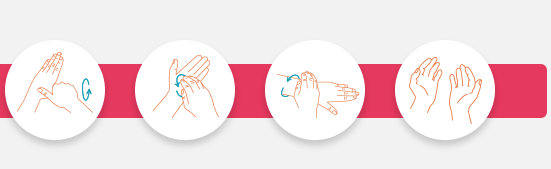
\includegraphics[width=.5\textwidth]{./imgs/img13.png}
\end{figure}

A principal recomendação é higienizar as mãos. São cuidados simples,
mas importantes e que devem ser frequentes para prevenir doenças
contagiosas.

Higienize as mãos frequentemente com água e sabão ou use antisséptico de
mãos à base de álcool gel 70\% {[}...{]}.

{[}...{]}

\textit{Ao tossir e espirrar}

\begin{figure}[htpb!]

\includegraphics[width=.5\textwidth]{./imgs/img14.png}
\end{figure}

Cubra a boca e o nariz. Use os braços ou lenço descartável. Evite usar
as mãos. E, se usar, lembre-se de higienizá-las.

{[}...{]}.

\fonte{São Paulo. SP contra o novo coronavírus. Disponível em: \emph{https://www.saopaulo.sp.gov.br/coronavirus/}.
Acesso em: 21 fev. 2023.}
\end{quote}

\num{6} Qual é o principal argumento encontrado nesse texto, publicado pelo governo do estado de São Paulo?

\reduline{O texto procura convencer o leitor da necessidade de combatermos a
transmissão do novo coronavírus com a higienização das mãos e os
cuidados a serem observados ao tossirmos ou espirrarmos.\hfill}
\linhas{1}


\num{7} Procure no texto e transcreva duas ações a serem realizadas contra o
coronavírus.

\reduline{De acordo com o texto, devemos higienizar as mãos constantemente e
cobrir a boca ao tossir ou espirrar.\hfill}
\linhas{2}


\num{8} Esse trecho do texto conta com duas imagens. Como elas se
relacionam aos argumentos apresentados?

\reduline{As imagens ensinam como os leitores devem lavar as mãos da forma correta e como
devem cobrir a boca ao tossir ou espirrar.\hfill}
\linhas{1}

\num{9} Que tipo de recurso, além da palavra escrita, um texto argumentativo
pode apresentar?

\reduline{Um texto argumentativo pode apresentar recursos visuais.\hfill}
\linhas{2}

\num{10} Por que é importante que um texto argumentativo traga também esses recursos?

\reduline{Um texto argumentativo pode lançar mão desse tipo de recurso para fortalecer o
ponto de vista defendido.\hfill}
\linhas{2}


\colorsec{Treino}

\num{1} Leia o texto.

\begin{quote}
\textbf{Vacina é vida!}

Vacinas salvam vidas, são seguras, não causam doenças e protegem a
comunidade! Segundo a Organização Mundial de Saúde, graças às vacinas
são evitadas, a cada ano, entre 2 e 3 milhões de mortes por doenças
preveníveis. Pensando nisso, o Instituto e a Fundação Butantan, em
parceria com a Sanofi Pasteur e a Secretaria Municipal de Educação de
São Paulo, com o apoio da Secretaria de Estado da Saúde de São Paulo e
da Secretaria Municipal de Saúde de São Paulo, promovem a Campanha “A
Importância da Vacinação.

{[}...{]}.

\fonte{Instituto Butantan. Campanha A importância da vacinação. Disponível em: \emph{https://campanhavacina.butantan.gov.br/}.
Acesso em: 21 fev. 2023.}
\end{quote}

Nesse texto, o argumento desenvolvido refere-se

\begin{minipage}{.5\textwidth}
\begin{escolha}
\item às etapas de fabricação das vacinas.

\item aos perigos associados à vacinação.

\item aos números da vacinação contra o coronavírus.

\item à importância da vacinação em geral.
\end{escolha}
\end{minipage}
\sidetext{Dificuldade: Fácil.

SAEB: Analisar o uso de recursos de persuasão em textos verbais e/ou
multimodais. BNCC: EF05LP20 -- Analisar a validade e força de argumentos
em argumentações sobre produtos de mídia para público infantil (filmes,
desenhos animados, HQs, games etc.), com base em conhecimentos sobre os
mesmos.}

\num{2} Leia o texto.

\begin{quote}
\textbf{As vacinas são seguras?}

As vacinas são muito seguras. É muito mais provável que sua criança seja
prejudicada por uma doença evitável por vacina do que por uma vacina.
Todas as vacinas passam por rigorosos testes de segurança, incluindo
estudos clínicos, antes de {[}serem{]} aprovadas para o público. Os países só
registram e distribuem vacinas que atendam a rigorosos padrões de
qualidade e segurança.

{[}...{]}.

\fonte{Unicef Brasil. Vacinas. Disponível em:\emph{https://www.unicef.org/brazil/vacinas-perguntas-e-respostas}.
Acesso em: 21 fev. 2023.}
\end{quote}

De acordo com o texto, um argumento forte para a vacinação é que

\begin{escolha}
\item são feitos rigorosos testes de segurança.

\item surgiu grande quantidade de doenças ultimamente.

\item estão disponível em baixo número os testes clínicos.

\item é baixa a probabilidade de uma criança ficar doente.
\end{escolha}

\coment{SAEB: Julgar a eficácia de argumentos em textos. BNCC: EF05LP20 -
Analisar a validade e força de argumentos em argumentações sobre
produtos de mídia para público infantil (filmes, desenhos animados, HQs,
games etc.), com base em conhecimentos sobre os mesmos.}

\num{3} Analise a imagem.

\begin{figure}[htpb!]

\includegraphics[width=.5\textwidth]{./imgs/img15.png}
%\caption{Fonte: http://www.fundacaocultural.ba.gov.br/2020/03/14210/Governo-do-Estado-anuncia-medidas-para-o-enfrentamento-ao-novo-coronavirus-Covid-19-na-Bahia.html. Acesso em: 21 fev. 2023.}
\end{figure}

De acordo com o cartaz, para combater o coronavírus, é preciso

\begin{escolha}
\item estimular a vacinação.

\item cumprimentar pessoas com aperto de mão.

\item higienizar bem as mãos.

\item evitar aglomerações.
\end{escolha}

\coment{SAEB: Analisar os efeitos de sentido de recursos multissemióticos em
textos que circulam em diferentes suportes. BNCC: EF05LP20 -- Analisar a
validade e força de argumentos em argumentações sobre produtos de mídia
para público infantil (filmes, desenhos animados, HQs, games etc.), com
base em conhecimentos sobre os mesmos.}

\chapter{Introdução à poesia}
\markboth{Módulo 5}{}

\vspace*{-2cm}

\coment{Habilidades da BNCC: EF35LP27, EF35LP31.}

\colorsec{Habilidades do SAEB}

\begin{itemize}
\item Reconhecer diferentes modos de organização composicional de textos em
versos.

\item Analisar a construção de sentidos de textos em versos com base em seus
elementos constitutivos.
\end{itemize}

\conteudo{Após estudarmos alguns gêneros textuais escritos em prosa, passemos
agora a uma modalidade artística diferente. A poesia é uma das formas
mais antigas da literatura. Ela permite que as palavras sejam arranjadas
de maneira criativa, impondo um ritmo e uma sonoridade e evocando
diferentes sensações nos leitores. Ela pode ser encontrada em várias
formas, como sonetos, haicais, poemas épicos, por exemplo.

\begin{wrapfigure}{l}{.5\textwidth}

\includegraphics[width=.5\textwidth]{./imgs/img16.jpg}
%\caption{Fonte: https://unsplash.com/pt-br/fotografias/PC-8bIgAVQg. Acesso em 21/03/2023.}
\end{wrapfigure}

Por meio da poesia, os escritores conseguem capturar o mundo ao seu
redor e, por exemplo, expressar suas emoções mais profundas. Trata-se de textos
baseados em uma visão individual transformada em forma literária. Em
outras palavras, a poesia se baseia em sentimentos que são transmitidos
ao leitor com o uso expressivo das palavras. Por esse motivo, ela tem
sido valorizada e apreciada ao longo dos séculos.

Cada linha de um poema é denominada \textbf{verso}. Essa seria a unidade básica
do texto. É a partir do verso que apreendemos as imagens e os
sentimentos expostos pelo poeta. Por sua vez, cada conjunto de versos é
denominado \textbf{estrofe}. É justamente a totalidade de versos, organizados ou
não em estrofes, que vai constituir o poema.

Quando há estrofes, dentro de cada uma, os versos normalmente são agrupados a partir de
um mesmo eixo temático. Ao unirmos o conteúdo de cada parte do poema,
extraímos, então, seu sentido geral. Analise o exemplo a seguir e perceba como,
em um poema, as linhas podem não ocupar uma linha inteira na página.}

\conteudo{
\begin{verse}
\textbf{Prece}

Senhor, a noite veio e a alma é vil.\\
Tanta foi a tormenta e a vontade!\\
Restam-nos hoje, no silêncio hostil,\\
O mar universal e a saudade.

Mas a chama, que a vida em nós criou,\\
Se ainda há vida ainda não é finda.\\
O frio morto em cinzas a ocultou:\\
A mão do vento pode erguê-la ainda.

Dá o sopro, a aragem --- ou desgraça ou ânsia ---,\\
Com que a chama do esforço se remoça,\\
E outra vez conquistemos a Distância ---\\
Do mar ou outra, mas que seja nossa!

\fonte{Fernando Pessoa. Prece. In: \emph{Mensagem.} São Paulo: Hedra, 2007.}
\end{verse}

\marginnote{\color{black}
\begin{tabular}{ll}
\textbf{Glossário} & \mbox{}\\
Ânsia & vontade.\\
Aragem & oportunidade.\\
Finda & terminada.\\
Hostil & desfavorável.\\
Remoçar & rejuvenescer.\\
Tormenta & tempestade.\\
Vil & desprezível.\\
\end{tabular}
}

Nesse poema de Fernando Pessoa, há três estrofes, e cada
uma contém quatro versos. É possível observarmos um
mesmo assunto sendo desenvolvido em cada uma delas:

\begin{itemize}
\item Na primeira estrofe, o poeta fala sobre a tristeza trazida pela noite.

\item Na segunda e na terceira estrofe, é mencionada uma chama capaz de manter a esperança e a vida
acesas.
\end{itemize}

Desse modo, ao lermos uma estrofe após a outra, conseguimos
extrair o sentido do poema como um todo, relacionando suas diferentes
partes.

Devemos destacar também o fato de muitos poemas apresentarem rimas. Elas
consistem na repetição sonora de uma ou mais palavras no final de dois
ou mais versos consecutivos. A função das rimas pode ser diversa, como:
estabelecer um padrão sonoro, criar musicalidade e ritmo, intensificar a
expressividade. Na primeira estrofe do poema de Fernando
Pessoa, encontramos rimas entre as palavras “vil” e “hostil” e entre “vontade”
e “saudade”. Dessa forma, percebemos como esse artifício é usado
para criar um sentido de musicalidade que estimula a declamação do
poema, ou seja, sua leitura em voz alta.}

\colorsec{Atividades}

\num{1} Como as palavras são organizadas em um poema?

\reduline{As palavras são arranjadas de forma criativa, impondo uma sonoridade e um ritmo.\hfill}
\linhas{2}

\num{2} Que diferença estrutural existe entre um texto em prosa e um poema?

\reduline{O texto em prosa é organizado em parágrafos, enquanto o poema é organizado em versos, que podem ser agrupados em estrofes.\hfill}
\linhas{1}

\num{3} Assinale V para o que for verdadeiro e F para o que for falso.

\begin{boxlist}
\boxitem{F} Um poema necessariamente não explora sonoridades.

\boxitem{V} Um poema pode ser declamado.

\boxitem{V} Os versos de uma estrofe costumam tratar de um mesmo tema.

\boxitem{F} Um poema não deve tratar de sentimentos.
\end{boxlist}

\num{4} Como chamamos a unidade básica do poema?

\reduline{O verso é a unidade básica do poema.\hfill}

\num{5} Complete a frase a seguir.

Um conjunto de versos constitui uma \reduline{estrofe\hfill}.

\num{6} Como chamamos o artifício poético que combina palavras com
sonoridades semelhantes?

\reduline{Chamamos de rima a combinação de palavras com terminações de sonoridades
iguais ou parecidas.\hfill}
\linhas{1}


\num{7} Por que o poeta lança mão desse artifício sonoro?

\reduline{As rimas expressam a musicalidade do poema, instigando sua declamação.\hfill}
\linhas{1}

\pagebreak
Leia o poema e responda às questões de 8 a 10.

\begin{minipage}{.5\textwidth}
\begin{verse}
\textbf{Canção do exílio}

Minha terra tem palmeiras\\
Onde canta o Sabiá,\\
As aves, que aqui gorjeiam,\\
Não gorjeiam como lá.

Nosso céu tem mais estrelas,\\
Nossas várzeas têm mais flores,\\
Nossos bosques têm mais vida,\\
Nossa vida mais amores.

Em cismar, sozinho, à noite,\\
Mais prazer encontro eu lá;\\
Minha terra tem palmeiras,\\
Onde canta o Sabiá.

Minha terra tem primores,\\
Que tais não encontro eu cá;\\
Em cismar -- sozinho, à noite --\\
Mais prazer encontro eu lá;\\
Minha terra tem palmeiras,\\
Onde canta o Sabiá.

Não permita Deus que eu morra,\\
Sem que eu volte para lá;\\
Sem que desfrute os primores\\
Que não encontro por cá;\\
Sem qu'inda aviste as palmeiras,\\
Onde canta o Sabiá.

\fonte{Gonçalves Dias. \emph{Cantos.} Leipzig: F. A. Brockhaus, 1857.}
\end{verse}
\end{minipage}\hspace{1cm}
\begin{minipage}{.5\textwidth}
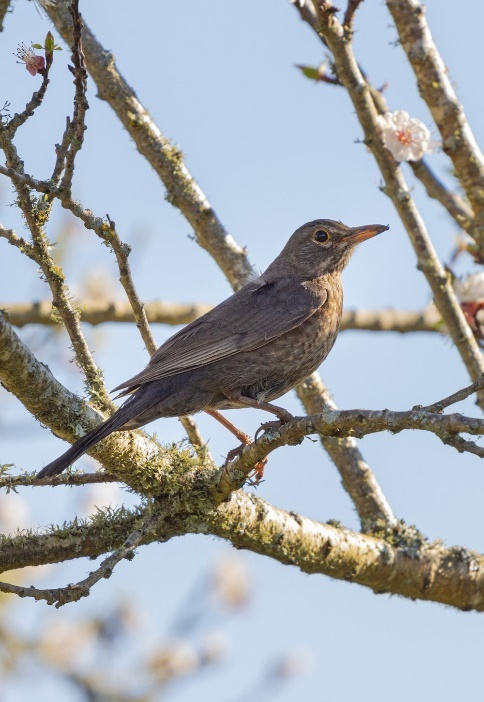
\includegraphics[width=\textwidth]{./imgs/img17.jpg}
%\caption{Sabiá. Fonte: https://unsplash.com/pt-br/fotografias/Ux0bFtZJnKw. Acesso em: 21 fev. 2023.}
\end{minipage}

\begin{tabular}{ll}
\textbf{Glossário} & \mbox{}\\
Gorjear & cantar.\\
Primor & perfeição.\\
Qu'inda & que ainda.\\
\end{tabular}

\pagebreak
\num{8} Sobre a estrutura do poema, responda:

\begin{escolha}
\item Quantas estrofes o poema apresenta?

\reduline{O poema está organizado em cinco estrofes.\hfill}
\linhas{1} 

\item Quantos versos há em cada estrofe?

\reduline{Cada uma das três primeiras estrofes contém quatro versos, enquanto cada uma das duas últimas estrofes contém seis versos.\hfill}
\end{escolha}


\num{9} Transcreva duas rimas do poema.

\reduline{Possibilidades de resposta: cá/sabiá; flores/amores.\hfill}
\linhas{1}


\num{10} Que tipo de sentimento a primeira estrofe do poema expressa?

\reduline{A primeira estrofe expressa um sentimento de tristeza, já que o poeta
fala da saudade que sente de sua terra.\hfill}


\colorsec{Treino}

\num{1} Leia um trecho de um poema.

\begin{verse}
\textbf{Saudades}

Nas horas mortas da noite\\
Como é doce o meditar\\
Quando as estrelas cintilam\\
Nas ondas quietas do mar;\\
Quando a lua majestosa\\
Surgindo linda e formosa,\\
Como donzela vaidosa\\
Nas águas se vai mirar!

Nessas horas de silêncio,\\
De tristezas e de amor,\\
Eu gosto de ouvir ao longe,\\
Cheio de mágoa e de dor,\\
O sino do campanário\\
Que fala tão solitário\\
Com esse som mortuário\\
Que nos enche de pavor.

{[}...{]}.

\fonte{Casimiro de Abreu. Saudades. In: \emph{Cantos de tristeza e
de saudade}. Paris: Casa Editorial Franco-Ibero-Americana, [s.d.].}
\end{verse}

\begin{tabular}{ll}
\textbf{Glossário} & \mbox{}\\
Campanário & torre.\\
Cintilar & brilhar.\\
Mirar & olhar.
\end{tabular}

Cada estrofe reproduzida apresenta

\begin{minipage}{.5\textwidth}
\begin{escolha}
\item oito versos.

\item dois versos.

\item versos sem rimas.

\item versos sem sentimentos.
\end{escolha}
\end{minipage}
\sidetext{SAEB: Reconhecer diferentes modos de organização composicional de textos
em versos. BNCC: EF35LP27 -- Ler e compreender, com certa autonomia,
textos em versos, explorando rimas, sons e jogos de palavras, imagens
poéticas (sentidos figurados) e recursos visuais e sonoros.}

\num{2} Leia um trecho de um poema.

\begin{verse}
\textbf{O canto do guerreiro}\\
\textbf{I}

Aqui na floresta\\
Dos ventos batida,\\
Façanhas de bravos\\
Não geram escravos,\\
Que estimem a vida\\
Sem guerra e lidar\\
--- Ouvi-me, Guerreiros,\\
--- Ouvi meu cantar.

{[}...{]}.

\fonte{Gonçalves Dias. O Canto do Guerreiro. In: \emph{Canto.}
Leipzig: F.A. Brockhaus, 1857.}
\end{verse}

Uma das rimas encontradas nessa estrofe é

\begin{minipage}{.5\textwidth}
\begin{escolha}
\item façanhas/não.

\item ouvi-me/ouvi.

\item lidar/cantar.

\item guerra/lidar.
\end{escolha}
\end{minipage}
\sidetext{SAEB: Reconhecer diferentes modos de organização composicional de textos
em versos. BNCC: EF35LP27 -- Ler e compreender, com certa autonomia,
textos em versos, explorando rimas, sons e jogos de palavras, imagens
poéticas (sentidos figurados) e recursos visuais e sonoros.}

\num{3} Leia um trecho de um poema.

\begin{verse}
\textbf{Sem remédio}

{[}...{]}

E é desde então que eu sinto este pavor,\\
Este frio que anda em mim, e que gelou\\
O que de bom me deu Nosso Senhor!\\
Se eu nem sei por onde ando e onde vou!

{[}...{]}.

\fonte{Florbela Espanca. Sem remédio. In: \emph{Poemas
selecionados.} São Paulo: Primavera Editorial, 2020.}
\end{verse}

Essa estrofe transmite um sentimento de

\begin{minipage}{.5\textwidth}
\begin{escolha}
\item alegria.

\item desespero.

\item aceitação.

\item entusiasmo.
\end{escolha}
\end{minipage}
\sidetext{SAEB: Analisar a construção de sentidos de textos em versos com base em
seus elementos constitutivos. BNCC: EF35LP31 -- Identificar, em textos
versificados, efeitos de sentido decorrentes do uso de recursos rítmicos
e sonoros e de metáforas.}

\chapter{Modos variados de se escrever e falar}
\markboth{Módulo 6}{}

\coment{Neste módulo, os alunos conhecerão o conceito de variedade linguística.
A ideia é compreender e diferenciar a língua culta das mais diferentes
formas de se comunicar, na fala e na escrita, considerando que apesar da
existência de normas, todas as manifestações linguísticas podem ser
consideradas válidas, trabalhando a ideia de preconceito linguístico.\\
Habilidades da BNCC: EF35LP22, EF35LP30.}

\colorsec{Habilidade do SAEB}

\begin{itemize}
\item Identificar as variedades linguísticas em textos.
\end{itemize}

\conteudo{Como qualquer outra língua, a língua portuguesa é muito diversa,
assim como toda a cultura dos povos que a utilizam, como o povo brasileiro.
Nas mais diferentes regiões do Brasil, por exemplo, é comum encontrarmos formas
diferentes de expressar um mesmo sentido. Podem-se
observar variações na pronúncia, no vocabulário e na sintaxe entre
diferentes regiões. Além disso, diferentes grupos sociais, como os jovens ou
as pessoas mais velhas, podem ter maneiras diferentes de se expressar,
usando gírias, expressões próprias e formas de falar específicas.

\begin{wrapfigure}{l}{.5\textwidth}
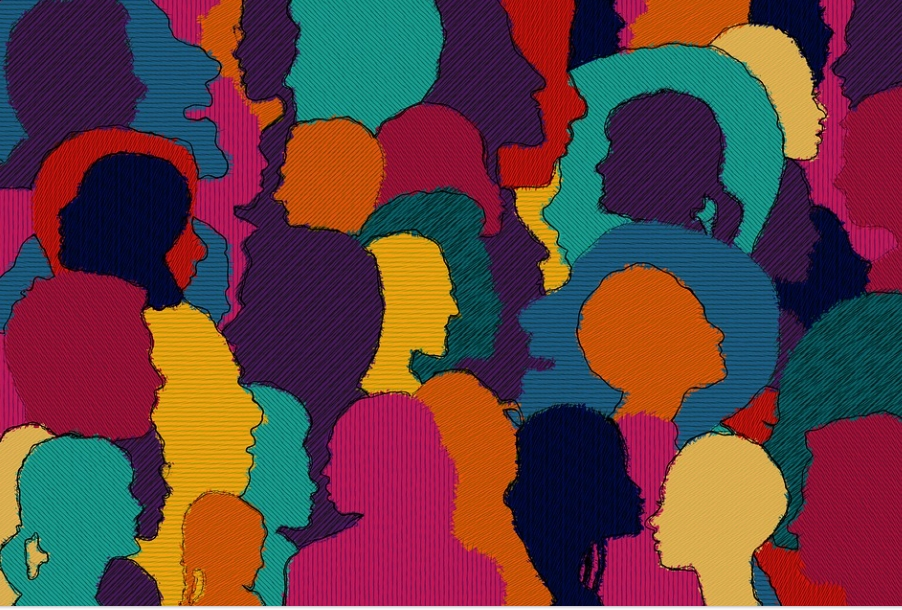
\includegraphics[width=.5\textwidth]{./imgs/img18.jpg}
%\caption{Fonte: https://pixabay.com/pt/illustrations/diversidade-pessoas-cabe\%c3\%a7as-humanos-5582454/. Acesso 26/02/2023.}
\end{wrapfigure}

Chamamos os conjuntos de formas diferentes de falar de \textbf{variedades
linguísticas}. Todas elas fazem parte da riqueza e da diversidade cultural
das diferentes comunidades que as falam e, por isso, devem ser respeitadas,
preservadas e valorizadas.
\vspace{1cm}}
\pagebreak

\colorsec{Atividades}

Leia o texto a seguir, do romance \emph{Inocência}, do escritor Visconde
de Taunay. Observe, durante a leitura, variações linguísticas. Depois, resolva as atividades de 1 a 6.

\begin{quote}
Chegou-se o pai à cama e, com todo o carinho, chamou: Nocência!
Nocência! E como não a visse despertar logo, sacudiua com brandura até
que ela abrisse uns olhos espantados.

--- Apre! Que sono! disse o bondoso velho. Num instante que fui lá
dentro?!... Vamos, são horas de tomar a mezinha. {[}...{]}

--- Olhe, dona, aconselhou ele, beba de um só trago e chupe, logo
depois, uns gomos de limão-doce.

--- Então é muito mau? choramingou a doente.

--- É amargo; mas num gole mecê toma isto.

--- Papai, recalcitrou a moça, não quero... eu não quero.

--- Ora, filhinha do meu coração, não se canhe; é preciso... Amanhã há
de você sentir-se boa; não é doutor?

--- Com certeza, se tomar esta poção, assegurou Cirino.

---Depois, quando eu ir lá à vila, hei de trazer para você uma coisa
bonita... uns lavrados. Ouviu?

--- Nhor-sim.

--- Ande, Tico, acrescentou o mineiro voltando-se para o anão, vai
depressa buscar limão-doce; na cozinha há um meio cascado.

\fonte{Visconde de Taunay. \emph{Inocência}. Disponível em:
\emph{http://objdigital.bn.br/Acervo\_Digital/livros\_eletronicos/inocencia.pdf}.
Acesso em: 26 fev. 2023.}
\end{quote}

\num{1} Após sua primeira leitura do texto, você acredita que o texto foi escrito
mais antigamente ou mais recentemente? Justifique sua resposta.

\reduline{Espera-se que os estudantes identifiquem o texto como escrito em uma
época passada a partir de marcas de variação linguística, como
“mecê” e “nhor-sim”, termos que não são mais ser utilizados atualmente.}
\linhas{1}


\num{2} Destaque alguns dos termos que você identificou, durante a sua
leitura, como variedades linguísticas.


\reduline{Resposta pessoal. Sugestões: apre, mecê, canhe, nhor-sim.}
\linhas{1}

\num{3} A partir de sua percepção sobre o contexto em que a história é
narrada, você diria que a cena se passa em uma área rural ou urbana? Por
quê?

\reduline{A cena se passa em uma área rural, pois o pai faz referência a ir “lá à
vila {[}...{]} trazer para você uma coisa bonita... uns lavrados”. Além
disso, podemos perceber pela linguagem dos personagens, como os termos “canhe” e
“cascado”, que se trata de um grupo sertanejo.}
\linhas{1}


\num{4} A palavra “lavrados” é um termo que no Brasil inteiro possui
vários sentidos bastante diferentes entre si. Sobre a explicação do sentido correto
para a palavra, tendo em vista o contexto da cena, assinale V para o que for verdadeiro e F para o que for falso.

\begin{boxlist}
\boxitem{F} Um campo “lavrado”, isto é, plantado e cultivado.

\boxitem{F} Um documento “lavrado” em cartório, isto é, registrado e estabelecido.

\boxitem{V} Um tecido “lavrado”, isto é, um tecido trabalhado e bordado para fazer vestido.

\boxitem{F} Um copo “lavrado”, isto é, um copo de material barato usado em bares.
\end{boxlist}

\num{5} Observe novamente o texto. A jovem “Nocência” (apelido de
Inocência) utiliza um pronome de tratamento, para se referir ao pai, que
pode ser considerado um caso de variação linguística.

\begin{escolha}
\item Escreva-o na linha a seguir.

\reduline{Nhor-sim.\hfill}

\item Qual é o seu significado?

\reduline{O termo é equivalente a “Sim, senhor”.\hfill}
\linhas{1}
\end{escolha}

\num{6} Releia este trecho retirado do diálogo do romance.

\begin{quote}
--- Apre! Que sono! disse o bondoso velho. Num instante que fui lá
dentro?!... Vamos, são horas de tomar a mezinha.
\end{quote}

Considerando que, nesse trecho, ocorrem marcas de discurso direto (isto é,
o texto reproduz a fala do personagem), identifique nessa fala uma
expressão utilizada por ele que pode ser considerado um caso de
variação linguística.

\reduline{A expressão “apre!”.\hfill}

\pagebreak

\num{7} Observe a foto a seguir.

\begin{figure}[htpb!]
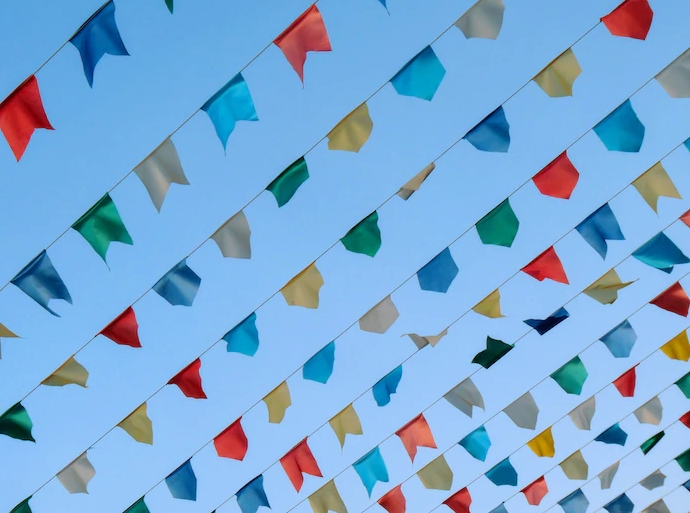
\includegraphics[width=.5\textwidth]{./imgs/img19.jpg}
\caption{Fonte: https://unsplash.com/pt-br/fotografias/UOAD9U-TYxc. Acesso em:: 26/02/2023.}
\end{figure}


Como costuma ser nomeado, na região em que você vive, o que está representado nessa imagem?
Complete a frase a seguir.\bigskip

As \preencher\preencher\preencher de São João representam uma decoração típica das
festas juninas no Brasil. São feitas de papel colorido e são penduradas
em fios ou cordas para decorar as ruas, praças e outros locais.

\coment{Possibilidades de resposta: bandeirola ou bandeirinha.}


\num{8} Observa esta imagem:

\begin{figure}[htpb!]
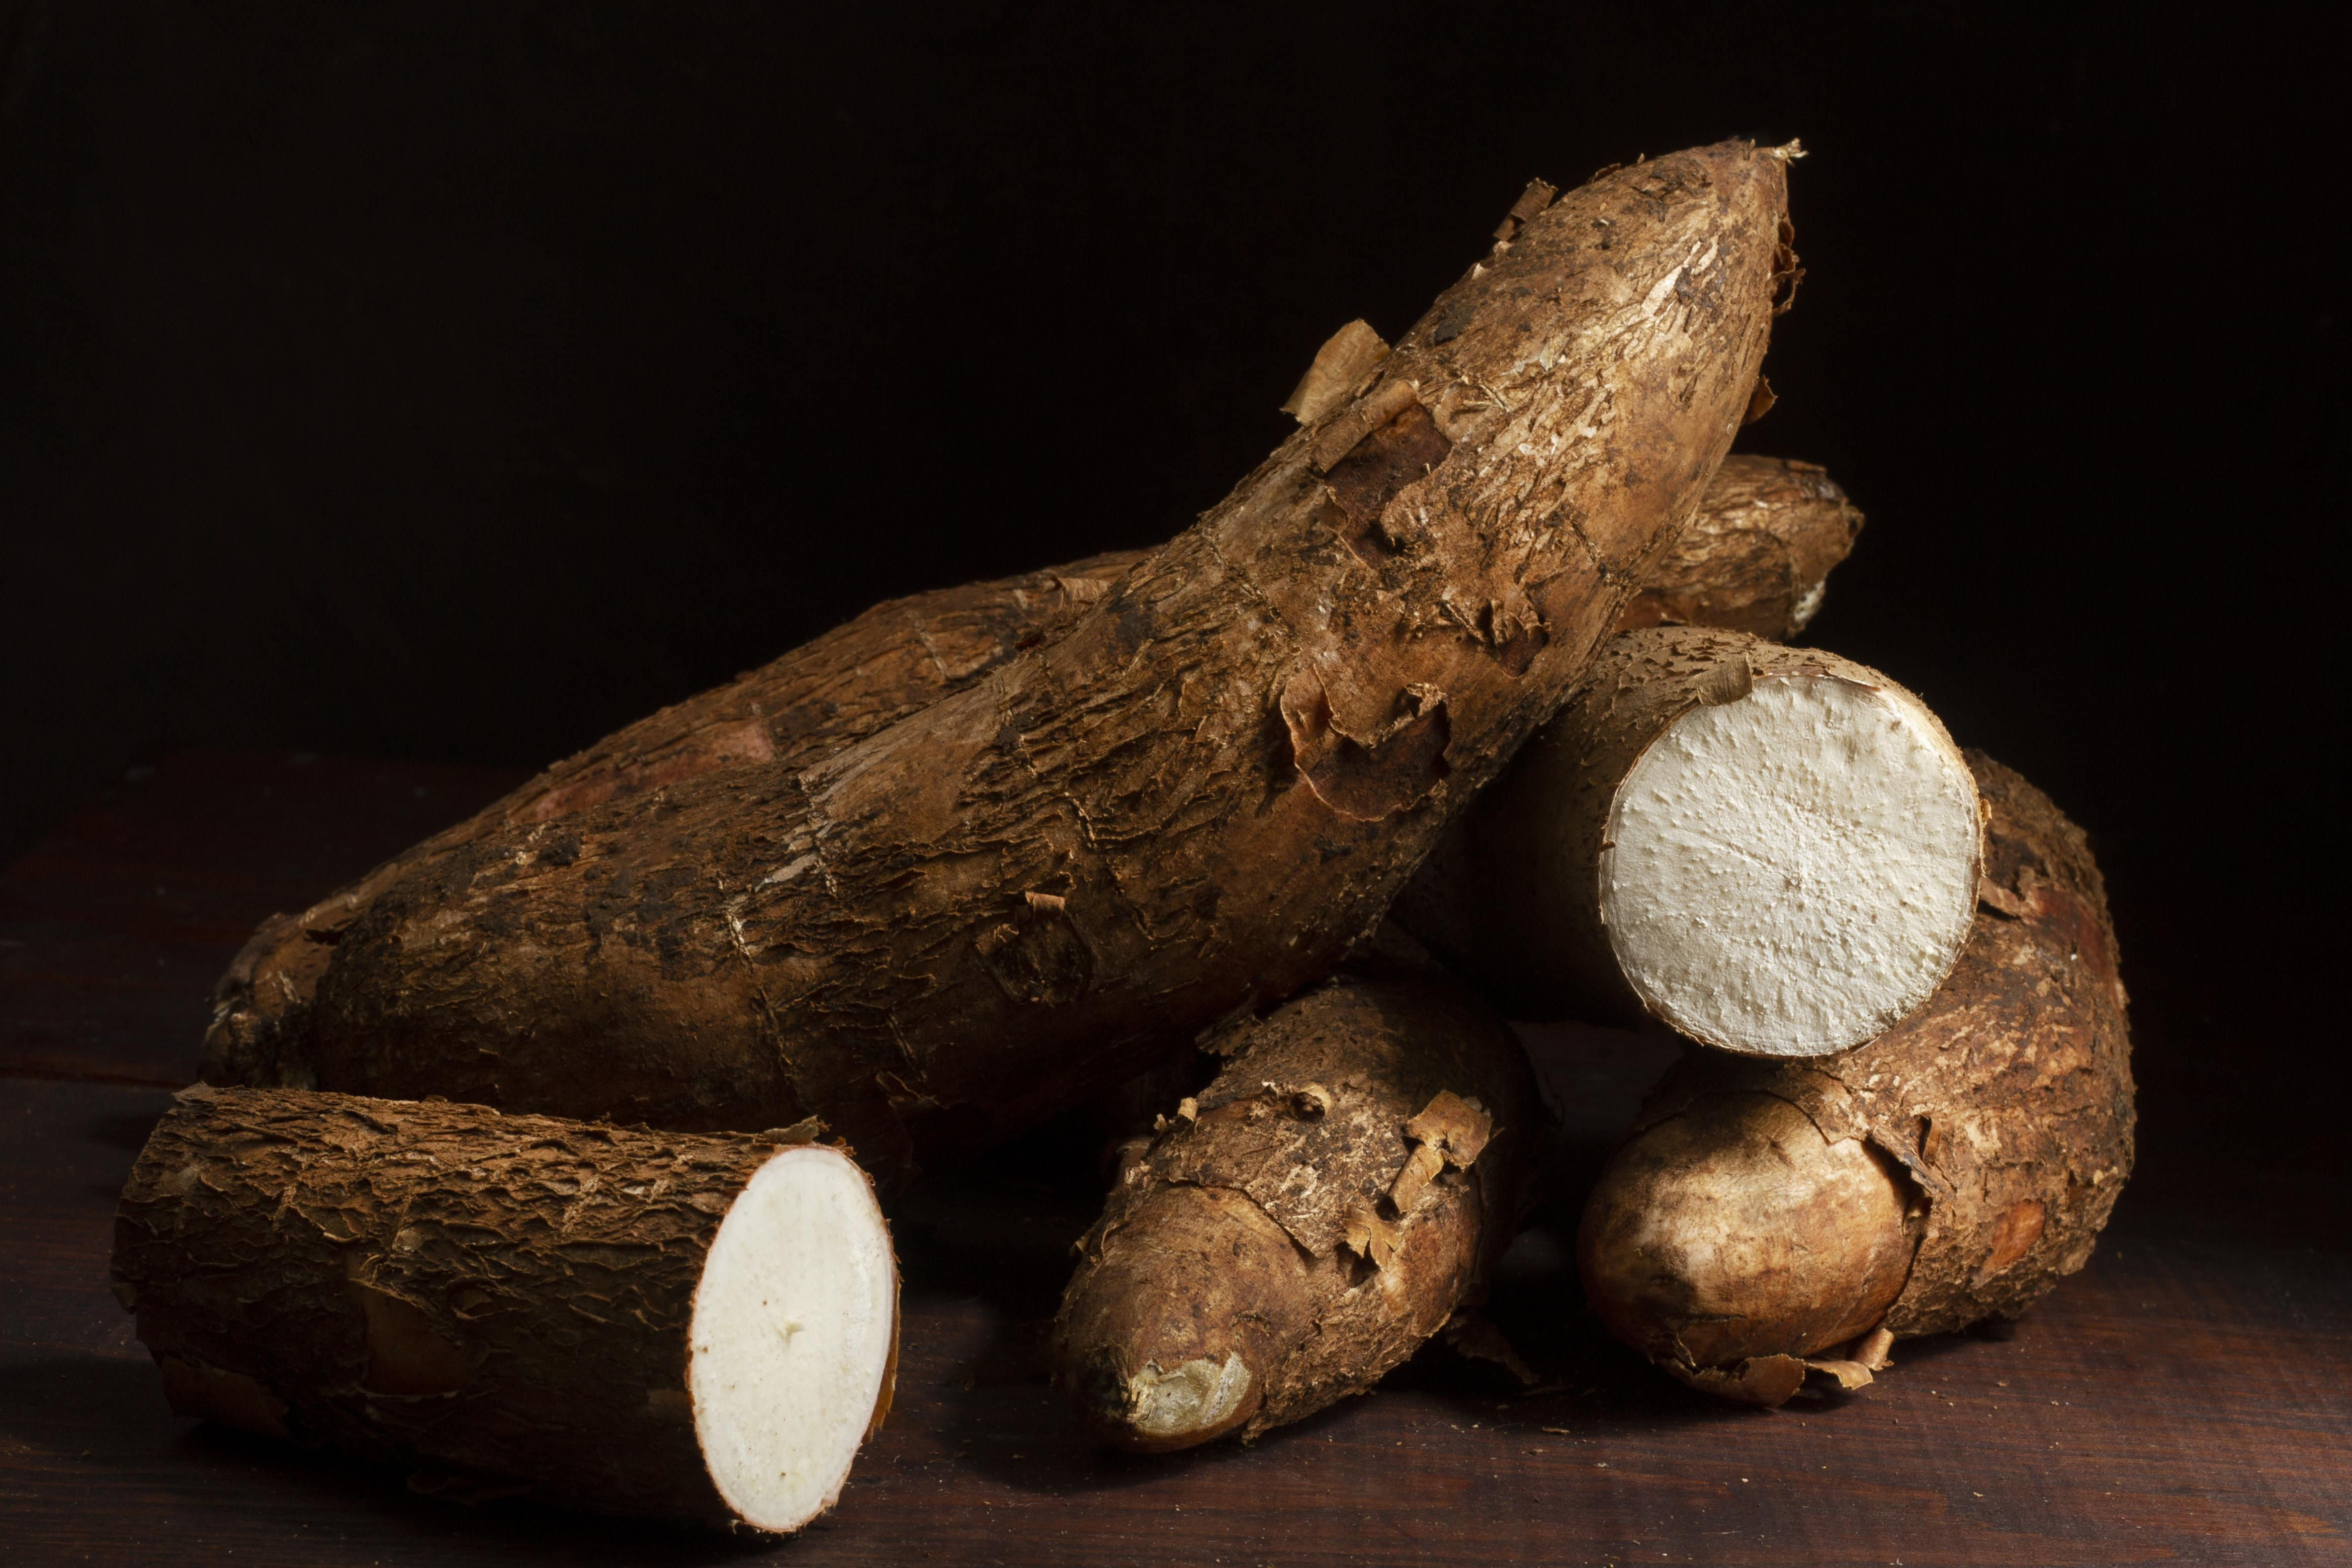
\includegraphics[width=.5\textwidth]{./imgs/img19b.jpg}
\caption{Fonte: https://unsplash.com/pt-br/fotografias/UOAD9U-TYxc. Acesso em: 26/02/2023.}
\end{figure}

O vegetal representado nessa imagem costuma ter diferentes nomes pelo Brasil.
Faça uma pesquisa e, depois, registre, a seguir, três nomes que esse vegetal recebe dependendo da região brasileira.

\reduline{São estes os nomes: mandioca, macaxeira ou aipim.\hfill}
\linhas{1}


\num{9} Complete as lacunas com exemplos de variação linguística para cada palavra ou expressão.

\begin{escolha}
\item Ônibus: \reduline{coletivo\hfill}

\item Refrigerante: \reduline{refri\hfill}

\item Pão francês:\reduline{pão de sal; cacetinho\hfill}

\item Pipoca: \reduline{poca; pipoquinha\hfill}
\end{escolha}


\num{10} A partir do tema estudado, responda: para você, qual é a importância de
aprender sobre variação linguística?

\reduline{Resposta pessoal. É importante que os estudantes percebam, por exemplo, que o
vocabulário se amplia com esse estudo de variedades linguísticas, além
de nos fazer ter uma percepção mais clara sobre as diferenças culturais
e sobre a importância do respeito a essas variedades, que são igualmente
válidas.\hfill}

\section{Treino}

\num{1} Leia o texto.

\begin{quote}
Cirino tomara a garrafa.

--- Isto, afirmou ele, acaba com certeza a cura.

E, esquivando-se de pronunciar o nome e a qualidade da pessoa de quem
estava tratando:

--- Ela há de ter hoje algum apetite e poderá levantar-se um pouco, pois
já tomou o seu caldinho.

--- Então, ao meio-dia, recomendou Pereira muito baixinho a Cirino,
vosmecê mande chamar a nossa doente e dê-lhe a \textbf{mezinha}. Ouviu?
Já avisei lá dentro...

\fonte{Visconde de Taunay. \emph{Inocência}. Disponível:
\emph{http://objdigital.bn.br/Acervo\_Digital/livros\_eletronicos/inocencia.pdf}.
Acesso em: 26 fev. 2023.}
\end{quote}

Selecione a alternativa que traz o significado correto da palavra “mezinha” (em destaque no texto).

\begin{escolha}
\item Pequena mesa utilizada por médicos para o tratamento de doenças leves.

\item Remédio caseiro fabricado com ingredientes naturais, como ervas e frutas.

\item Espécie de vela utilizada em barcos grandes para regular as direções seguidas.

\item Andar intermediário localizado entre dois andares principais de um prédio.
\end{escolha}

\coment{SAEB: Identificar as variedades linguísticas em textos. BNCC:EF35LP05- Inferir o sentido de palavras ou expressões desconhecidas em textos, com base no contexto da frase ou do texto.}

\num{2} Leia o texto.

\begin{quote}
Levantou uns olhos súplices e, agarrando resolutamerte o remédio,
bebeu-o todo de um jacto. Depois deu um suspiro de enjôo e ficou com os
lábios entreabertos, à espera que o adocicado sumo do limão lhe tirasse
o amargor do medicamento.

--- Então, exclamou Pereira, era maior o medo que a coisa em si! Você
tomou a dose numa \textbf{relancina}.

\fonte{Visconde de Taunay. \emph{Inocência}. Disponível:
\emph{http://objdigital.bn.br/Acervo\_Digital/livros\_eletronicos/inocencia.pdf}.
Acesso em: 26 fev. 2023.}
\end{quote}

A palavra em destaque, “relancina”, é um regionalismo
utilizado no Rio Grande do Sul. Selecione a alternativa que indica um sinônimo
para a expressão “numa relancina”.

\begin{minipage}{.5\textwidth}
\begin{escolha}
\item Rapidamente.

\item Lentamente.

\item Dificilmente.

\item Pausadamente.
\end{escolha}
\end{minipage}
\sidetext{SAEB: Identificar as variedades linguísticas em textos. BNCC:EF35LP05- Inferir o sentido de palavras ou expressões desconhecidas em textos, com base no contexto da frase ou do texto.}

\num{3} Leia o texto.

\begin{quote}
Ouvira Meyer estas indicações terapêuticas com os olhos muito fitos em
quem as dava: depois, voltando-se para Pereira, disse com um aprobatório
aceno de cabeça:

--- \textbf{Pom} médico! \textbf{pom} médico!

Desse momento em diante, votou Cirino ao alemão a mais decidida da
simpatia; e Pereira, presenciando o congraçamento daqueles dois homens,
de si para si ilustres e incontestáveis sabichões, sentiu-se feliz por
abrigá-los a um tempo em sua humilde vivenda.

\fonte{Visconde de Taunay. \emph{Inocência}. Disponível:
\emph{http://objdigital.bn.br/Acervo\_Digital/livros\_eletronicos/inocencia.pdf}.
Acesso em: 26 fev. 2023.}
\end{quote}

O termo em destaque “pom” aparece como \textbf{discurso direto} do
personagem estrangeiro. Esse termo indica que o

\begin{escolha}
\item narrador escreve de maneira diferente da fala do personagem,
corrigindo sua fala.

\item personagem fala exatamente dessa forma, pois é discurso direto,
e assim se mostra sua pronúncia.

\item narrador insere uma fala para o personagem mostrando um sentido
diferente e contrário.

\item trecho não reproduz exatamente a fala do personagem alemão,
pois é discurso direto.
\end{escolha}

\coment{SAEB: Identificar as variedades linguísticas em textos. BNCC: EF35LP30 -- Diferenciar discurso indireto e discurso direto, determinando o efeito de sentido de verbos de enunciação e explicando o uso de variedades linguísticas no discurso direto, quando for
o caso.}

\chapter{Palavras que acrescentam sentidos}
\markboth{Módulo 7}{}

\coment{Os alunos serão apresentados a duas classes de palavras: adjetivos e
advérbios. Nesse momento, é importante compreender que essas palavras
acrescentam sentidos às outras, não tendo, em geral, uma existência independente
nos textos lidos.}

\colorsec{Habilidades do SAEB}

\begin{itemize}
\item Analisar os efeitos de sentido decorrentes do uso dos adjetivos.

\item Analisar os efeitos de sentido decorrentes do uso dos advérbios.
\end{itemize}

\begin{figure}[htpb!]
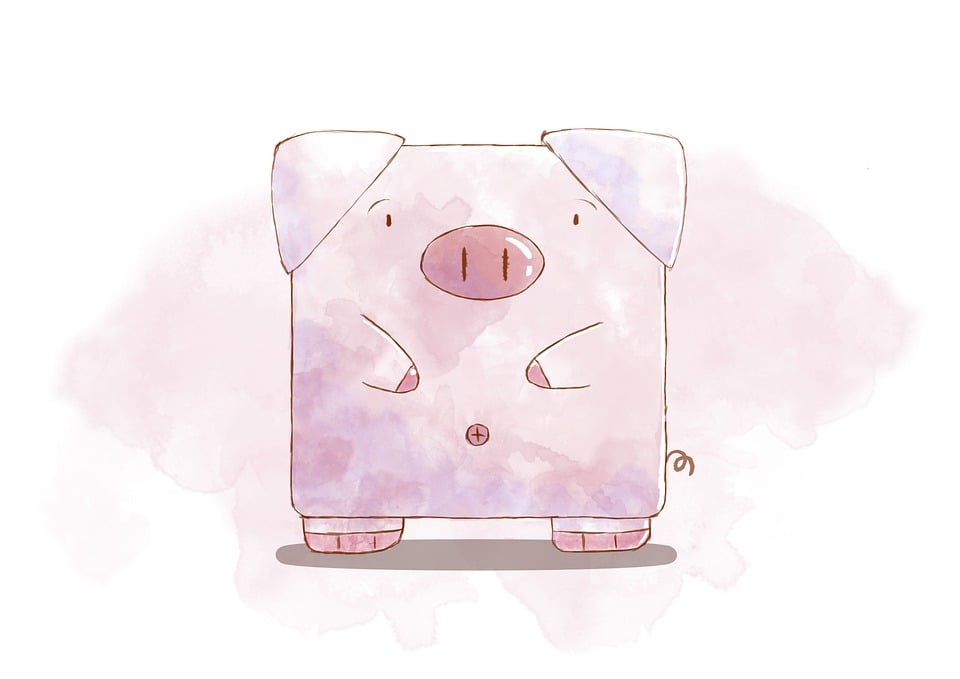
\includegraphics[width=.5\textwidth]{./imgs/img20.jpg}
%\caption{Fonte: https://pixabay.com/pt/illustrations/porco-porco-de-desenho-animado-4417320/}
\end{figure}

\conteudo{Existem diversas maneiras de nos expressarmos textualmente. Quando
contamos uma história, é comum pensarmos em torná-la mais atraente e
descritiva. Uma forma importante de fazer isso é por meio de duas
classes de palavras: os \textbf{adjetivos} e os \textbf{advérbios}.

\begin{itemize}
\item
  O adjetivo caracteriza um substantivo,
  propriedades como cor, tamanho, forma, origem,
  estado, entre outras. Por exemplo: o vestido \textit{azul}; o cachorro
  \textit{grande}; a casa \textit{antiga}; o menino \textit{feliz}.
\item
  O advérbio modifica ou complementa o sentido de um verbo, um adjetivo ou
  outro advérbio, indicando circunstâncias como tempo, modo, lugar,
  intensidade, negação, afirmação, entre outras. Por exemplo: ela
  correu \textit{rapidamente}; ele cantou \textit{muito bem}; nós vamos sair \textit{agora};
  eles \textit{nunca} chegaram atrasados.
\end{itemize}
}

\colorsec{Atividades}

Leia o texto e resolva as atividades de 1 a 10.

\begin{quote}
\textbf{Os três porquinhos}

Era uma vez três porquinhos aventureiros: o primeiro era preguiçoso e
gostava de dormir o dia todo, o segundo era vaidoso e passava horas se
admirando no espelho, e o terceiro era trabalhador e sempre ocupado
construindo sua casa com muito cuidado.

Um dia, um grande e malvado lobo apareceu na floresta, procurando uma
refeição saborosa para satisfazer sua fome voraz. O lobo farejou o ar e
logo sentiu o cheiro suculento dos porquinhos. Ele seguiu o cheiro até a
primeira casa, construída com palha e capim. O porquinho preguiçoso
dormia profundamente e nem sequer notou o lobo se aproximando. O lobo
soprou e soprou, até que a casa se desfez em pedaços, e o porquinho
preguiçoso fugiu correndo para a casa do segundo porquinho.

A casa do segundo porquinho era um pouco melhor, construída com madeira,
mas ainda assim era bastante frágil. O lobo chegou logo em seguida,
ansioso para devorar seu jantar. O lobo soprou e soprou, mas a casa
aguentou mais tempo do que a primeira. Porém, ainda assim, não resistiu e
o porquinho preguiçoso e o porquinho vaidoso tiveram de fugir para a casa
do terceiro porquinho.

A casa do terceiro porquinho era a mais forte de todas, feita de tijolos
sólidos e resistentes. Quando o lobo chegou, ele não conseguiu soprar a
casa e não conseguiu entrar pela porta, que estava trancada. O porquinho
trabalhador havia construído uma casa resistente e segura, protegendo a
si mesmo e a seus irmãos dos perigos da floresta.

O lobo tentou enganar o porquinho esperto, mas ele não caiu em suas
mentiras e permaneceu firme em sua casa forte. O lobo, finalmente,
desistiu e foi embora para procurar outra refeição. Assim, os porquinhos
puderam viver seguros, sem medo dos perigos que espreitavam na floresta.

\fonte{Texto escrito para este material.}
\end{quote}


\num{1} Qual é a personalidade de cada um dos três porquinhos?

\reduline{Cada personagem é caracterizado por um adjetivo: o primeiro porquinho é
preguiçoso, o segundo é vaidoso e o terceiro é trabalhador.\hfill}
\linhas{2}


\num{2} Como essa caracterização influencia a história?

\reduline{Essa caracterização influencia a história, pois é a personalidade de
cada um dos porquinhos que determina a qualidade da casa que eles
constroem e sua capacidade de resistir ao ataque do lobo.\hfill}
\linhas{2}


\num{3} De que maneira os adjetivos que explicam as personalidades dos
porquinhos auxiliam o leitor a diferenciá-los entre si?

\reduline{Os adjetivos utilizados ajudam a diferenciar suas personalidades e a
mostrar como cada um deles reage diante do perigo e da ameaça do lobo.
Enquanto o primeiro e o segundo porquinho não dão muita importância à
construção de uma casa forte e resistente, o terceiro porquinho é
retratado como alguém responsável e cuidadoso.\hfill}
\linhas{2}


\num{4} Retome no texto a descrição das casas dos três porquinhos. Como as
três casas são descritas?

\reduline{A primeira casa é descrita como sendo feita de palha e capim; a segunda
casa é feita de madeira; a terceira casa é feita de tijolos.\hfill}
\linhas{2}


\num{5} De que maneira os adjetivos utilizados para descrever as três casas
contribuem para fazer o leitor entender o andamento da história?

\reduline{A primeira casa de palha é entendida como frágil, podendo ser atacada
pelo lobo. A segunda é entendida como mais resistente, mas não o
suficiente para suportar o sopro do lobo. Já a casa de tijolos é sólida
e resistente, o que a torna a mais forte de todas e capaz de resistir ao
ataque do lobo.\hfill}
\linhas{3}


\num{6} Como as descrições das casas contribuem para a criação de um
ambiente e de uma atmosfera específicos na narrativa?

\reduline{A primeira casa (de palha) transmite uma sensação de fragilidade, criando
um ambiente de perigo e de ameaça. A segunda casa (de madeira) transmite
uma sensação de resistência e de esperança, mas ainda assim há a
sensação de perigo. Já a descrição da terceira casa como sendo feita de
tijolos sólidos e resistentes transmite uma sensação de proteção,
criando um ambiente de tranquilidade e segurança.\hfill}
\linhas{3}

\num{7} Cite advérbios usados no conto “Os três porquinhos”.

\reduline{Exemplos de advérbios utilizados no conto são: “profundamente”,
“logo”, “mais”, “bastante”, “firmemente” e “finalmente”.\hfill}


\num{8} Relacione as colunas entre os advérbios e as funções que eles
exercem ao longo do conto.

\begin{multicols}{2}
(1) Profundamente\medskip

(2) Logo\medskip

(3) Bastante\medskip

(4) Mais

\columnbreak

({\rosa{3}}) Quantidade.\medskip

({\rosa{2}}) Tempo.\medskip

({\rosa{4}}) Modo.\medskip

({\rosa{1}}) Intensidade.
\end{multicols}

\num{9} Na frase “O lobo soprou e soprou, até que a casa se desfez em
pedaços”, qual é a função do advérbio “até”?

\reduline{O advérbio “até” é usado para descrever a continuidade da ação, que se
interrompe em certo limite, indicando que o lobo soprou repetidamente
até o momento em que a casa se quebrou completamente.\hfill}
\linhas{1}


\num{10} Retome o conto. Qual é o sentido do advérbio “profundamente”?

\reduline{O advérbio “profundamente” descreve como o porquinho preguiçoso estava
dormindo quando o lobo chegou: “O porquinho preguiçoso dormia
profundamente e nem sequer notou o lobo se aproximando.” Esse advérbio
ajuda a dar ênfase na preguiça do porquinho, além de indicar que ele
estava dormindo de maneira muito intensa.\hfill}
\linhas{2}

\section{Treino}

Leia o texto para responder às questões de 1 a 3.

\begin{verse}
\textbf{A avó}

A avó, que tem oitenta anos,\\
Está tão fraca e velhinha!...\\
Teve tantos desenganos!\\
Ficou branquinha, branquinha,\\
Com os desgostos humanos.


Hoje, na sua cadeira,\\
Repousa, pálida e fria,\\
Depois de tanta canseira:\\
E cochila todo o dia,\\
E cochila a noite inteira.


Às vezes, porém, o bando\\
Dos netos invade a sala...\\
Entram rindo e papagueiando:\\
Este briga, aquele fala,\\
Aquele dança, pulando...


A velha acorda sorrindo.\\
E a alegria a transfigura;\\
Seu rosto fica mais lindo,\\
Vendo tanta travessura,\\
E tanto barulho ouvindo.


Chama os netos adorados,\\
Beija-os, e, tremulamente,\\
Passa os dedos engelhados,\\
Lentamente, lentamente,\\
Por seus cabelos doirados.


Fica mais moça, e palpita,\\
E recupera a memória,\\
Quando um dos netinhos grita:\\
“Ó vovó! conte uma história!\\
Conte uma história bonita!”


Então, com frases pausadas,\\
Conta histórias de quimeras,\\
Em que há palácios de fadas,\\
E feiticeiras, e feras,\\
E princesas encantadas ...


E os netinhos estremecem,\\
Os contos acompanhando,\\
E as travessuras esquecem,\\
- Até que, a fronte inclinando\\
Sobre o seu colo, adormecem...
\end{verse}
\fonte{Olavo Bilac. Poesias infantis. Rio de Janeiro: Francisco Alves, 1929. Disponível em: \emph{https://www.unicamp.br/iel/memoria/Ensaios/LiteraturaInfantil/Poesias\%20Infantis/Pi01.htm}. Acesso em: 25 mar. 2023.}

\num{1} Os adjetivos empregados nas duas primeiras estrofes para caracterizar a avó reforçam a ideia de que ela.

\begin{escolha}
\item vive uma idade vigorosa.

\item está fragilizada pela idade.

\item é forte e viçosa como uma jovem.

\item considera-se mais forte que os jovens.
\end{escolha}

\coment{SAEB: Analisar os efeitos de sentido decorrentes do uso dos adjetivos.}


\num{2} No verso “Seu rosto fica mais lindo”, o adjetivo

\begin{escolha}
\item indica que os netos importunam a avó.

\item denota que a avó não se importa com os netos.

\item marca que ocorre uma transformação no estado da avó.

\item demonstra que a avó não consegue mais reagir ao mundo.
\end{escolha}

\coment{SAEB: Analisar os efeitos de sentido decorrentes do uso dos adjetivos.}


\num{3} Releia esta estrofe.

\begin{verse}
Chama os netos adorados,\\
Beija-os, e, tremulamente,\\
Passa os dedos engelhados,\\
Lentamente, lentamente,\\
Por seus cabelos doirados.
\end{verse}

Os advérbios presentes nessa estrofe reforçam a ideia de que a avó está

\begin{escolha}
\item jovem e alerta.

\item velha e cansada.

\item saudosa e alegre.

\item infeliz e raivosa.
\end{escolha}

\coment{SAEB: Analisar os efeitos de sentido decorrentes do uso dos advérbios.}

\chapter{Fatos e opiniões}
\markboth{Módulo 8}{}

\coment{Neste módulo, os alunos vão entrar em contato com as diferenças entre
fatos e opiniões. É importante estabelecer essa diferenciação, pois ela
permite reconhecer \emph{fake news} e ainda suscita um diálogo saudável
e mais produtivo em sala de aula e na vida em sociedade.\\
Habilidades da BNCC: EF05LP16.}

\colorsec{Habilidades do SAEB}

\begin{itemize}
\item Distinguir fatos de opiniões em textos.

\item Avaliar a fidedignidade de informações sobre um mesmo fato veiculadas
em diferentes mídias.
\end{itemize}

\conteudo{Em nossa comunicação cotidiana, é muito comum que nos deparemos com
fatos e opiniões. Você sabe qual é a diferença entre eles?

\begin{wrapfigure}{l}{.4\textwidth}
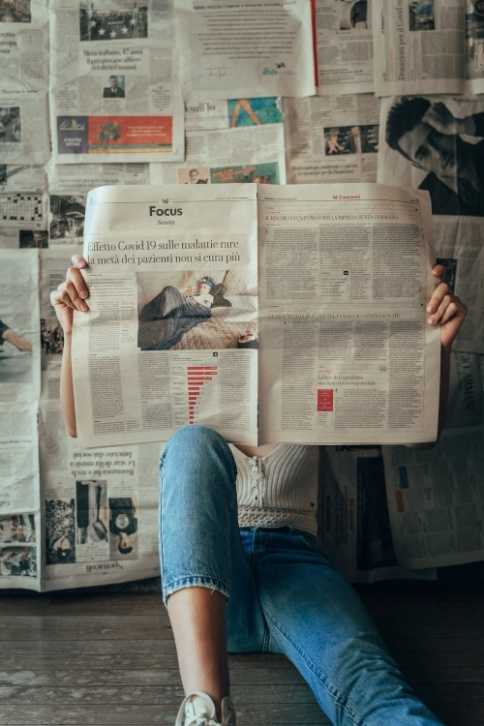
\includegraphics[width=.4\textwidth]{./imgs/img21.jpg}
%\caption{Fonte: https://unsplash.com/pt-br/fotografias/Bc\_y35IwUHw. Acesso 20/02/2023.}
\end{wrapfigure}

\textbf{Fatos} são informações objetivas que podem ser comprovadas por evidências
ou dados verificáveis. Assim, eles são baseados em observações e
medidas e não dependem de crenças pessoais ou pontos de vista. Podemos
considerar exemplos de fatos a temperatura de um local, o número de
habitantes de uma cidade ou o resultado de uma eleição.

\textbf{Opiniões} refletem nossos pensamentos, crenças ou
sentimentos pessoais. Assim, são subjetivas e podem variar de pessoa
para pessoa, pois cada uma tem sua própria experiência de vida e seus
valores, emoções e até mesmo preconceitos. Por esse motivo, você pode
achar uma comida gostosa, que seu amigo acha ruim, ou ele pode
gostar de um filme de que você não gosta.

É muito importante distinguir fatos de opiniões porque, quando as pessoas
confundem os dois conceitos, elas podem transmitir informações imprecisas ou mesmo
falsas, o que pode levar a mal-entendidos ou decisões equivocadas. Além
disso, essa distinção garante um debate saudável e uma sociedade mais informada.}


\colorsec{Atividades}

Leia o texto para resolver as atividades de 1 a 10.

\begin{quote}
\textbf{O link mais visto no Facebook}

No relatório do Facebook, de 2021, com os links mais vistos na rede social
entre janeiro e março daquele ano, aparece aquele que levava à notícia
de um jornal americano atribuindo a morte de um médico à vacina contra
o novo coronavírus. A afirmação era falsa.

O texto tornou-se um alarde e ficou popular, principalmente entre as pessoas
envolvidas em movimentos negacionistas contra vacinação. Entre o momento em
que a notícia foi divulgada e o momento em que o jornal atualizou o texto --
informando que nova análise apontava que não havia ligação evidente entre a
vacinação e a morte do médico duas semanas depois de ele ter se vacinado --,
a notícia falsa rodou o mundo.

Segundo o relatório do próprio Facebook, o link para essa notícia alcançou
a marca de 54.000.000 de visualizações de usuários da rede social.

Em paralelo, o Centro de Controle de Doenças do Departamento de Saúde dos Estados
Unidos afirma testes clínicos e pesquisas realizados aos montes apontam que as
vacinas contra o novo coronavírus são todas seguras e eficazes. Apesar disso, a
fama que o link alcançou está relacionada com ativistas antivacinas, muito atuantes
no Facebook, que se mostrou um território fértil para esse tipo de conteúdo.

Na tentativa de impedir que as pessoas se vacinassem contra o novo coronavírus,
os movimentos negacionistas espalhavam, no Facebook, histórias emotivas, como
a do médico que teria morrido por conta da vacina, e essa se mostrava uma
tática eficaz.

Nunca é demais salientar que, em todos os casos de pessoas que morreram
mesmo vacinadas contra o novo coronavírus, nunca foi encontrada uma evidência
de que a vacina estivesse relacionada à causa da morte.

\fonte{Fonte de pesquisa: BBC. Vacina contra Covid-19: notícia errada vira link
mais compartilhado pelo Facebook nos EUA. Disponível em: \emph{https://www.bbc.com/portuguese/internacional-58312501}. Acesso em: 25 mar. 2023.}
\end{quote}


\num{1} Qual foi a notícia mais compartilhada no Facebook nos Estados
Unidos no primeiro trimestre de 2021?

\reduline{Uma notícia no site de um jornal americano que atribuía equivocadamente
a morte de um médico à vacina contra o novo coronavírus.\hfill}
\linhas{1}


\num{2} Por que essa notícia foi considerada equivocada?

\reduline{Porque a análise de peritos apontou não haver evidências de que a
vacinação tivesse causado a morte do homem.\hfill}
\linhas{1}


\num{3} Qual foi a correção feita na matéria?

\reduline{A matéria foi atualizada para informar que não havia evidências de que a
vacinação tivesse causado a morte do médico.\hfill}
\linhas{1}


\num{4} Por que o link se tornou popular entre movimentos negacionistas
antivacina?

\reduline{Isso ocorreu, porque os adeptos desses movimentos encontram no Facebook
um ambiente fértil para a distribuição desse tipo de conteúdo e porque promovem
histórias emotivas para impedir as pessoas de serem vacinadas.\hfill}
\linhas{1}


\num{5} Quantas visualizações o link teve no total?

\reduline{Foram 54 milhões de visualizações de usuários do Facebook.\hfill}
\linhas{1}


\num{6} O que o Centro de Controle de Doenças do Departamento de Saúde dos Estados
Unidos afirma sobre as vacinas contra o novo coronavírus?

\reduline{O Centro de Controle de Doenças do Departamento de Saúde dos Estados Unidos
afirma que as vacinas são seguras e eficazes.\hfill}
\linhas{1}


\num{7} Por que a ampla disseminação do link no Facebook tem relação com uma
rede de ativistas antivacina?

\reduline{Essa relação existe, porque esses ativistas encontram no Facebook um ambiente fértil para
a distribuição desse tipo de conteúdo.\hfill}
\linhas{1}


\num{8} Qual tem sido uma das principais táticas desses grupos para impedir
as pessoas de serem vacinadas?

\reduline{Promover histórias emotivas, como a do médico, cuja morte foi equivocadamente atribuída
à vacina contra o novo coronavírus.\hfill}
\linhas{1}


\num{9} Podemos entender, de acordo com o texto, que as notícias falsas são
propagadas por fatos ou por opiniões? Justifique sua resposta.

\reduline{As notícias falsas são propagadas por opiniões, pois são baseadas em
histórias que não encontram validação na realidade, sem embasamento em dados objetivos.\hfill}


\num{10} Em sua opinião, de que maneira a disseminação de notícias falsas
impacta a busca por medidas de saúde mais eficazes?

\reduline{Resposta pessoal. Espera-se que os alunos compreendam que as notícias
falsas podem gerar grandes malefícios, danos e até mesmo a morte de
muitas pessoas, nos casos de se voltarem aos temas de saúde e ciência.\hfill}
\linhas{2}

\colorsec{Treino}

Releia o texto para responder às questões de 1 a 3.\medskip

\begin{minipage}{.5\textwidth}
\begin{quote}
\textbf{O link mais visto no Facebook}

No relatório do Facebook, de 2021, com os links mais vistos na rede social
entre janeiro e março daquele ano, aparece aquele que levava à notícia
de um jornal americano atribuindo a morte de um médico à vacina contra
o novo coronavírus. A afirmação era falsa.

O texto tornou-se um alarde e ficou popular, principalmente entre as pessoas
envolvidas em movimentos negacionistas contra vacinação. Entre o momento em
que a notícia foi divulgada e o momento em que o jornal atualizou o texto --
informando que nova análise apontava que não havia ligação evidente entre a
vacinação e a morte do médico duas semanas depois de ele ter se vacinado --,
a notícia falsa rodou o mundo.
\end{quote}
\end{minipage}\hspace{1cm}
\begin{minipage}{.5\textwidth}
\includegraphics[width=\textwidth]{./imgs/img21b.jpg}
\end{minipage}

\begin{quote}
Segundo o relatório do próprio Facebook, o link para essa notícia alcançou
a marca de 54.000.000 de visualizações de usuários da rede social.

Em paralelo, o Centro de Controle de Doenças do Departamento de Saúde dos Estados
Unidos afirma testes clínicos e pesquisas realizados aos montes apontam que as
vacinas contra o novo coronavírus são todas seguras e eficazes. Apesar disso, a
fama que o link alcançou está relacionada com ativistas antivacinas, muito atuantes
no Facebook, que se mostrou um território fértil para esse tipo de conteúdo.

Na tentativa de impedir que as pessoas se vacinassem contra o novo coronavírus,
os movimentos negacionistas espalhavam, no Facebook, histórias emotivas, como
a do médico que teria morrido por conta da vacina, e essa se mostrava uma
tática eficaz.

Nunca é demais salientar que, em todos os casos de pessoas que morreram
mesmo vacinadas contra o novo coronavírus, nunca foi encontrada uma evidência
de que a vacina estivesse relacionada à causa da morte.

\fonte{Fonte de pesquisa: BBC. Vacina contra Covid-19: notícia errada vira link
mais compartilhado pelo Facebook nos EUA. Disponível em: \emph{https://www.bbc.com/portuguese/internacional-58312501}.
Acesso em: 25 mar. 2023.}
\end{quote}

\num{1} Segundo o texto, qual é a explicação para a ampla
disseminação, no Facebook, da notícia errada sobre a vacina contra o novo coronavírus?

\begin{escolha}
\item A notícia falsa foi patrocinada por grandes empresas farmacêuticas,
que querem controlar a narrativa em torno das vacinas.

\item A notícia falsa foi compartilhada por engano por usuários inocentes
do Facebook.

\item A notícia falsa foi compartilhada por ativistas antivacina, que
encontram no Facebook um ambiente fértil.

\item A notícia falsa foi divulgada por políticos que se opõem à vacinação contra covid-19.
\end{escolha}

\coment{SAEB: Avaliar a fidedignidade de informações sobre um mesmo fato veiculadas em diferentes mídias. BNCC:
EF05LP16 -- Comparar informações sobre um mesmo fato veiculadas em diferentes mídias e concluir sobre qual é mais confiável e por quê.}

\num{2} Qual é o objetivo principal do artigo sobre a notícia errada da vacina
contra o novo coronavírus?

\begin{escolha}
\item Mostrar que a vacinação contra a covid-19 pode causar morte.

\item Explicar como o Facebook pode ser usado para espalhar desinformação.

\item Argumentar que as pessoas não devem confiar nas vacinas contra a covid-19.

\item Defender que a notícia errada foi compartilhada por ativistas pró-vacinação.
\end{escolha}

\coment{SSAEB: Avaliar a fidedignidade de informações sobre um mesmo fato veiculadas em diferentes mídias. BNCC:
EF05LP16 -- Comparar informações sobre um mesmo fato veiculadas em diferentes mídias e concluir sobre qual é mais confiável e por quê.}

\num{3} Qual é o objetivo do Centro de Controle de Doenças do Departamento de Saúde dos Estados
Unidos em relação às vacinas contra a Covid-19?

\begin{escolha}
\item Desencorajar as pessoas a tomarem as vacinas.

\item Estimular a ampla disseminação de notícias falsas sobre as vacinas.

\item Defender a segurança e a eficácia das vacinas contra a covid-19.

\item Ignorar as pesquisas com dados populacionais sobre as vacinas.
\end{escolha}

\coment{SAEB: Distinguir fatos de opiniões em textos. BNCC: EF05LP16 -- Comparar
informações sobre um mesmo fato veiculadas em diferentes mídias e concluir sobre
qual é mais confiável e por quê.}

\chapter{Organizando dados}
\markboth{Módulo 9}{}

\coment{Os alunos serão apresentados a dois modos bastante comuns de organizar
dados: os gráficos e as tabelas. É importante que compreendam como ambos
se organizam e as facilidades que eles trazem para a organização e a
compreensão de dados, pois são formas de organizar dados de maneira
visualmente facilitada.\\
Habilidade da BNCC: EF05LP23.}

\colorsec{Habilidade do SAEB}

\begin{itemize}
\item Analisar informações apresentadas em gráficos, infográficos ou tabelas.
\end{itemize}

\begin{figure}[htpb!]
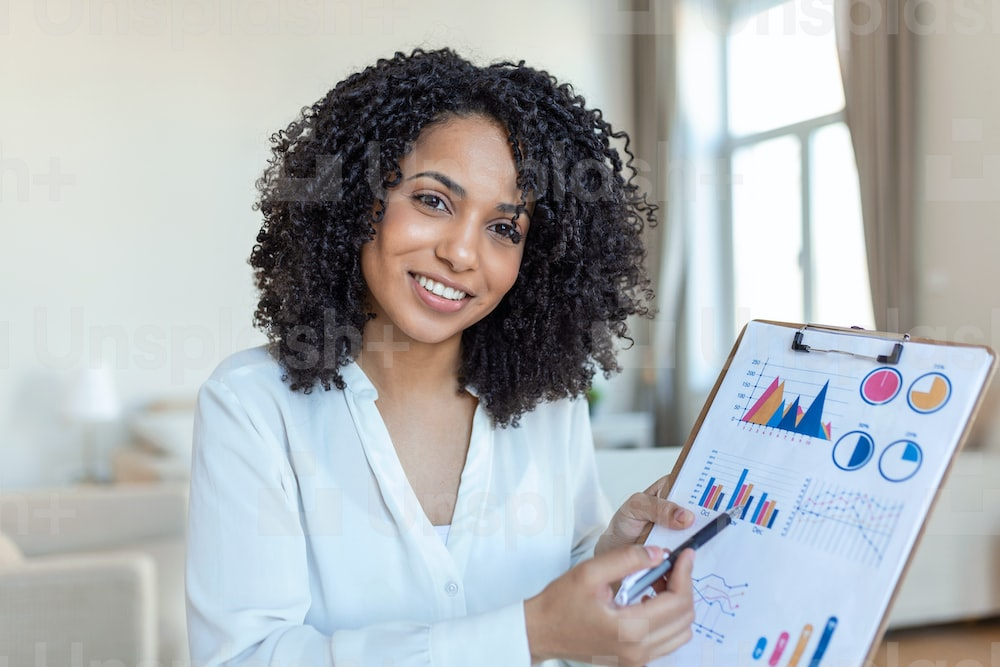
\includegraphics[width=.5\textwidth]{./imgs/img22.jpg}
%\caption{Fonte: https://unsplash.com/pt-br/fotografias/Jy2mwPtOCOU}
\end{figure}

\conteudo{Você já ouviu falar em gráficos? Sabe para que servem? Os gráficos são
ferramentas muito úteis para nos ajudar a entender informações
importantes. Eles são como desenhos que mostram dados de uma forma fácil
de entender.

Por exemplo, se quisermos saber quantas pessoas, em determinado grupo, gostam de sorvete de chocolate e
quantas pessoas preferem o sabor de baunilha, podemos fazer uma pesquisa e colocar
os resultados em um gráfico. Veja:

\begin{wrapfigure}{l}{.5\textwidth}
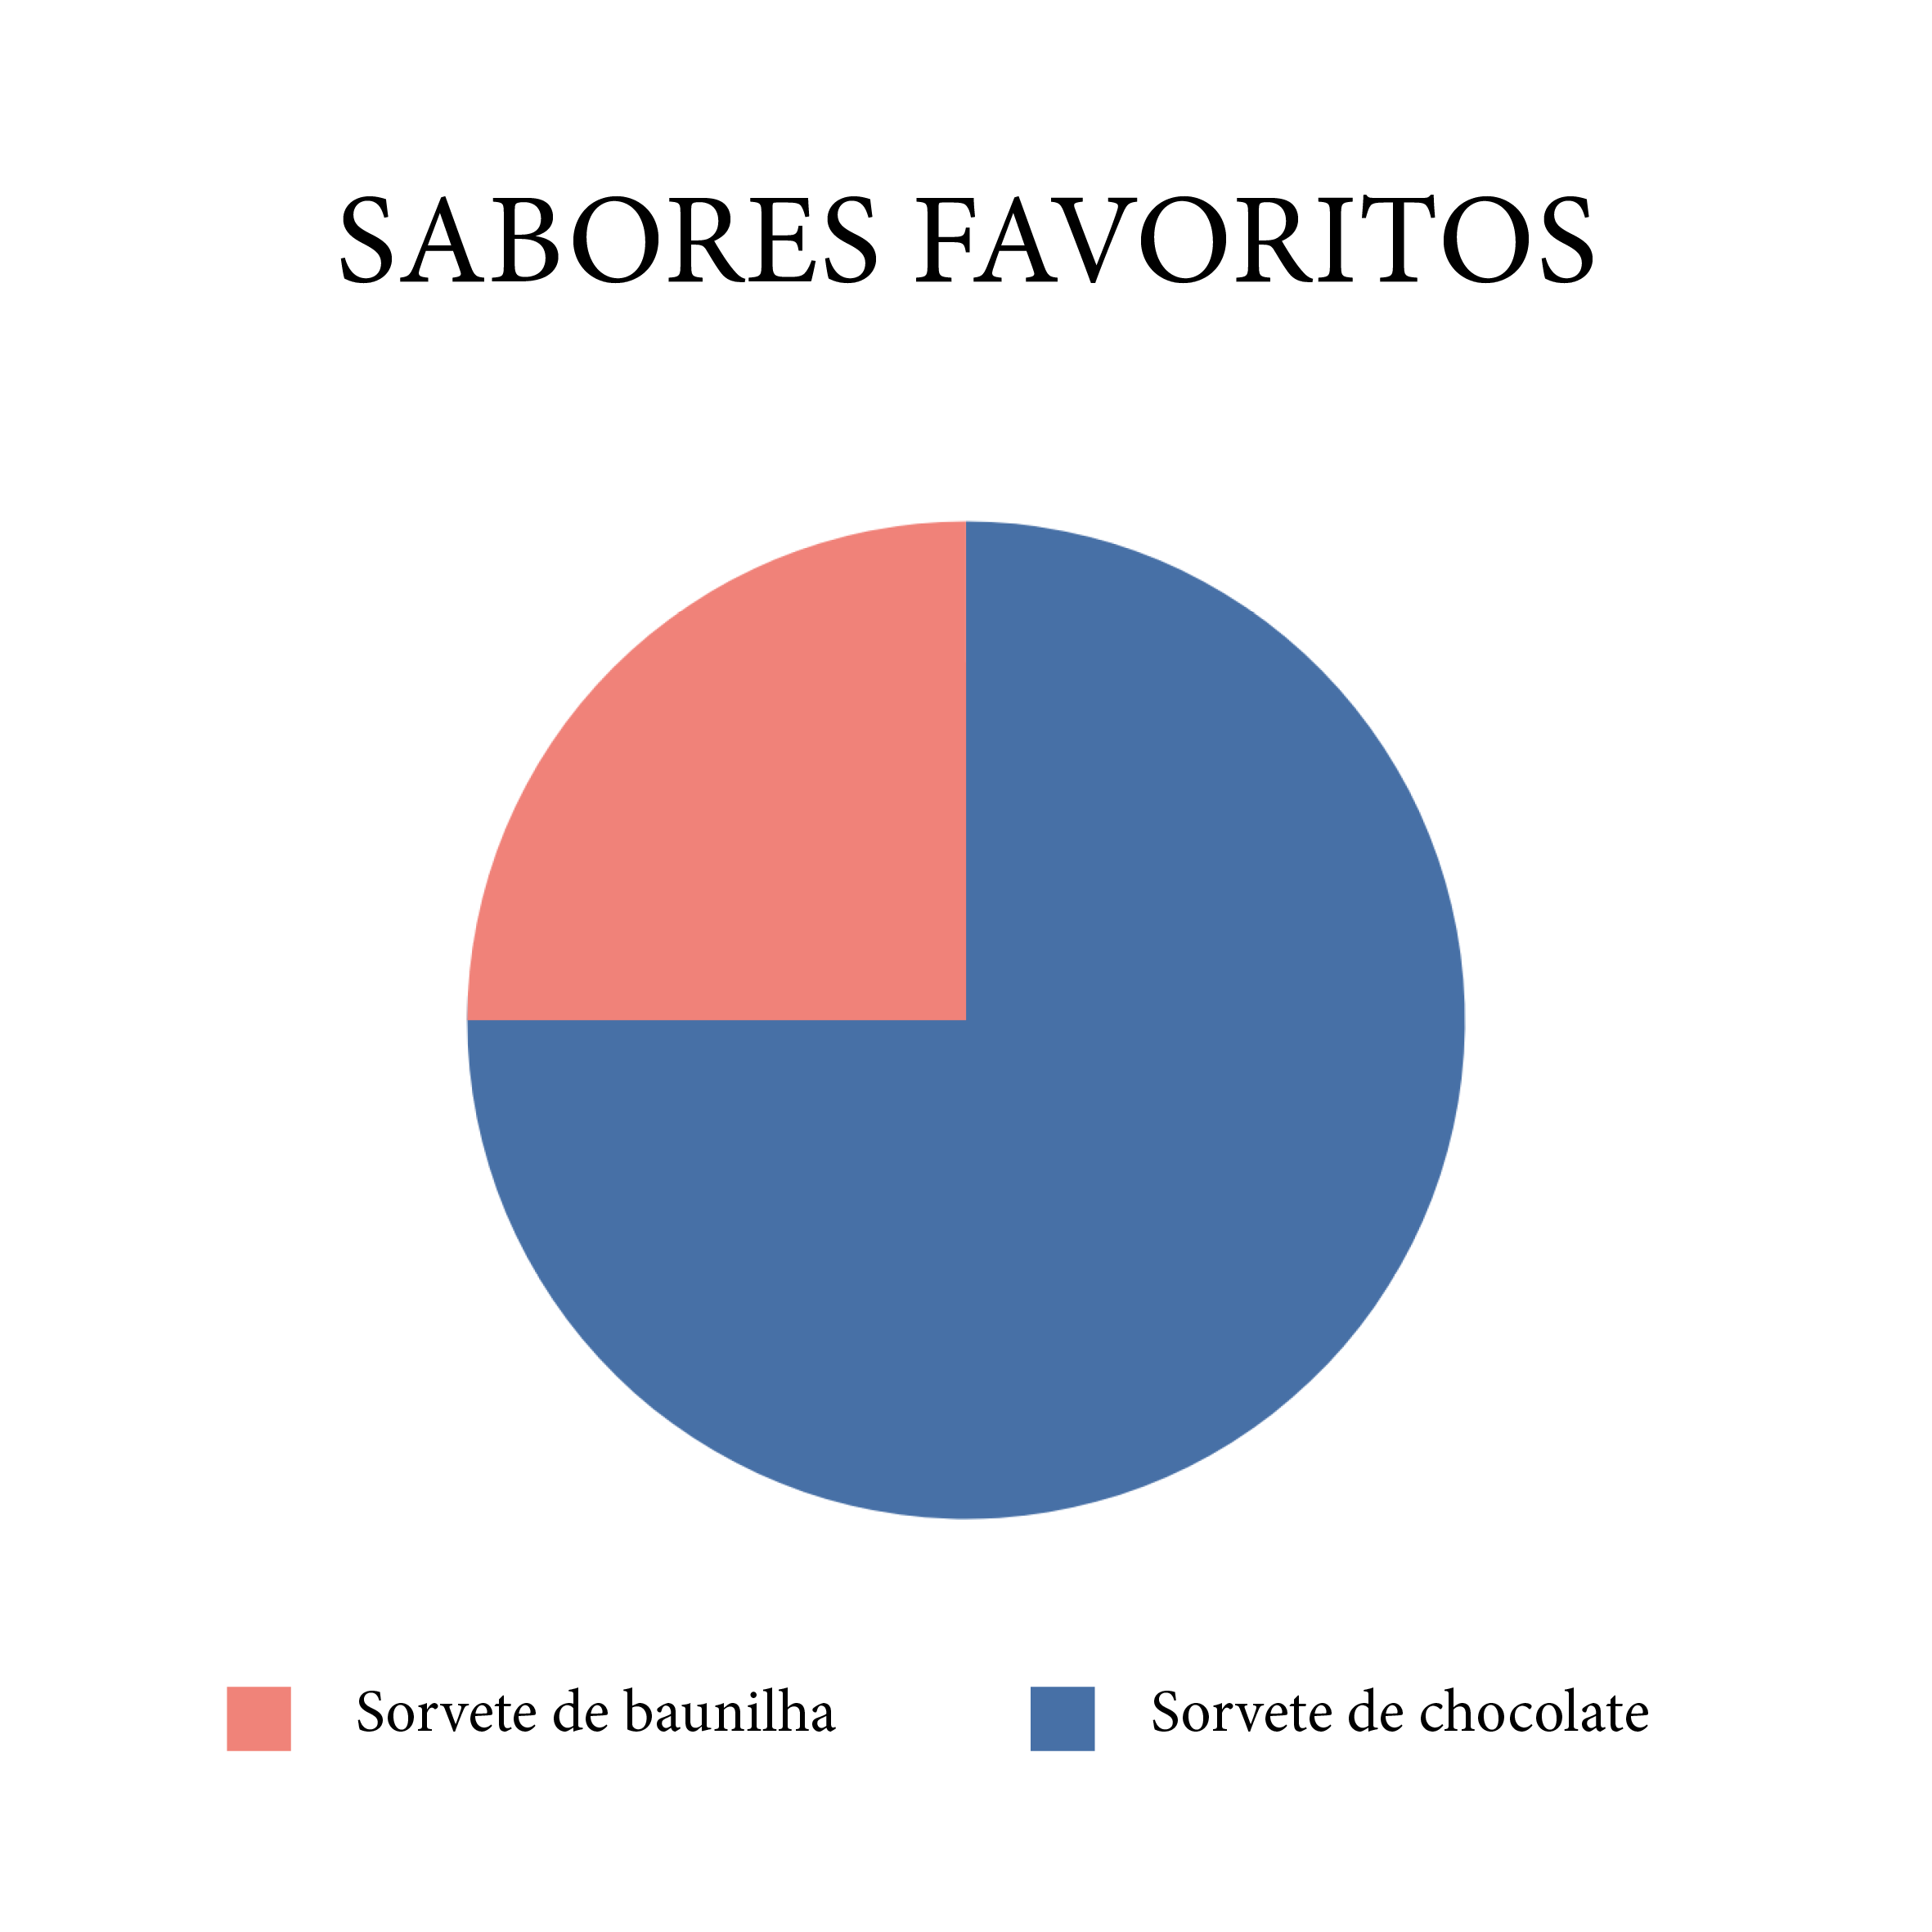
\includegraphics[width=.5\textwidth]{../ilustracoes/POR5/SAEB_5ANO_POR_FIGURA1.png}
\end{wrapfigure}
}

\conteudo{
Esse tipo de gráfico é denominado pizza, porque tem o formato de uma e cada parte do gráfico é como que uma fatia.
A pizza inteira representa a totalidade de pessoas pesquisadas. A fatia maior representa as pessoas que preferem sorvete de chocolate, e a fatia menor representa as pessoas que preferem sorvete de baunila. Observe como, no gráfico, essas informações ficam bem visualmente simplificadas.

Os gráficos são parecidos com desenhos e ajudam a ver como os dados
estão distribuídos. Por exemplo, se quisermos saber a quantidade de
frutas que foram vendidas em uma loja durante um mês, podemos fazer um
gráfico de barras. Veja:

\begin{wrapfigure}{l}{.5\textwidth}
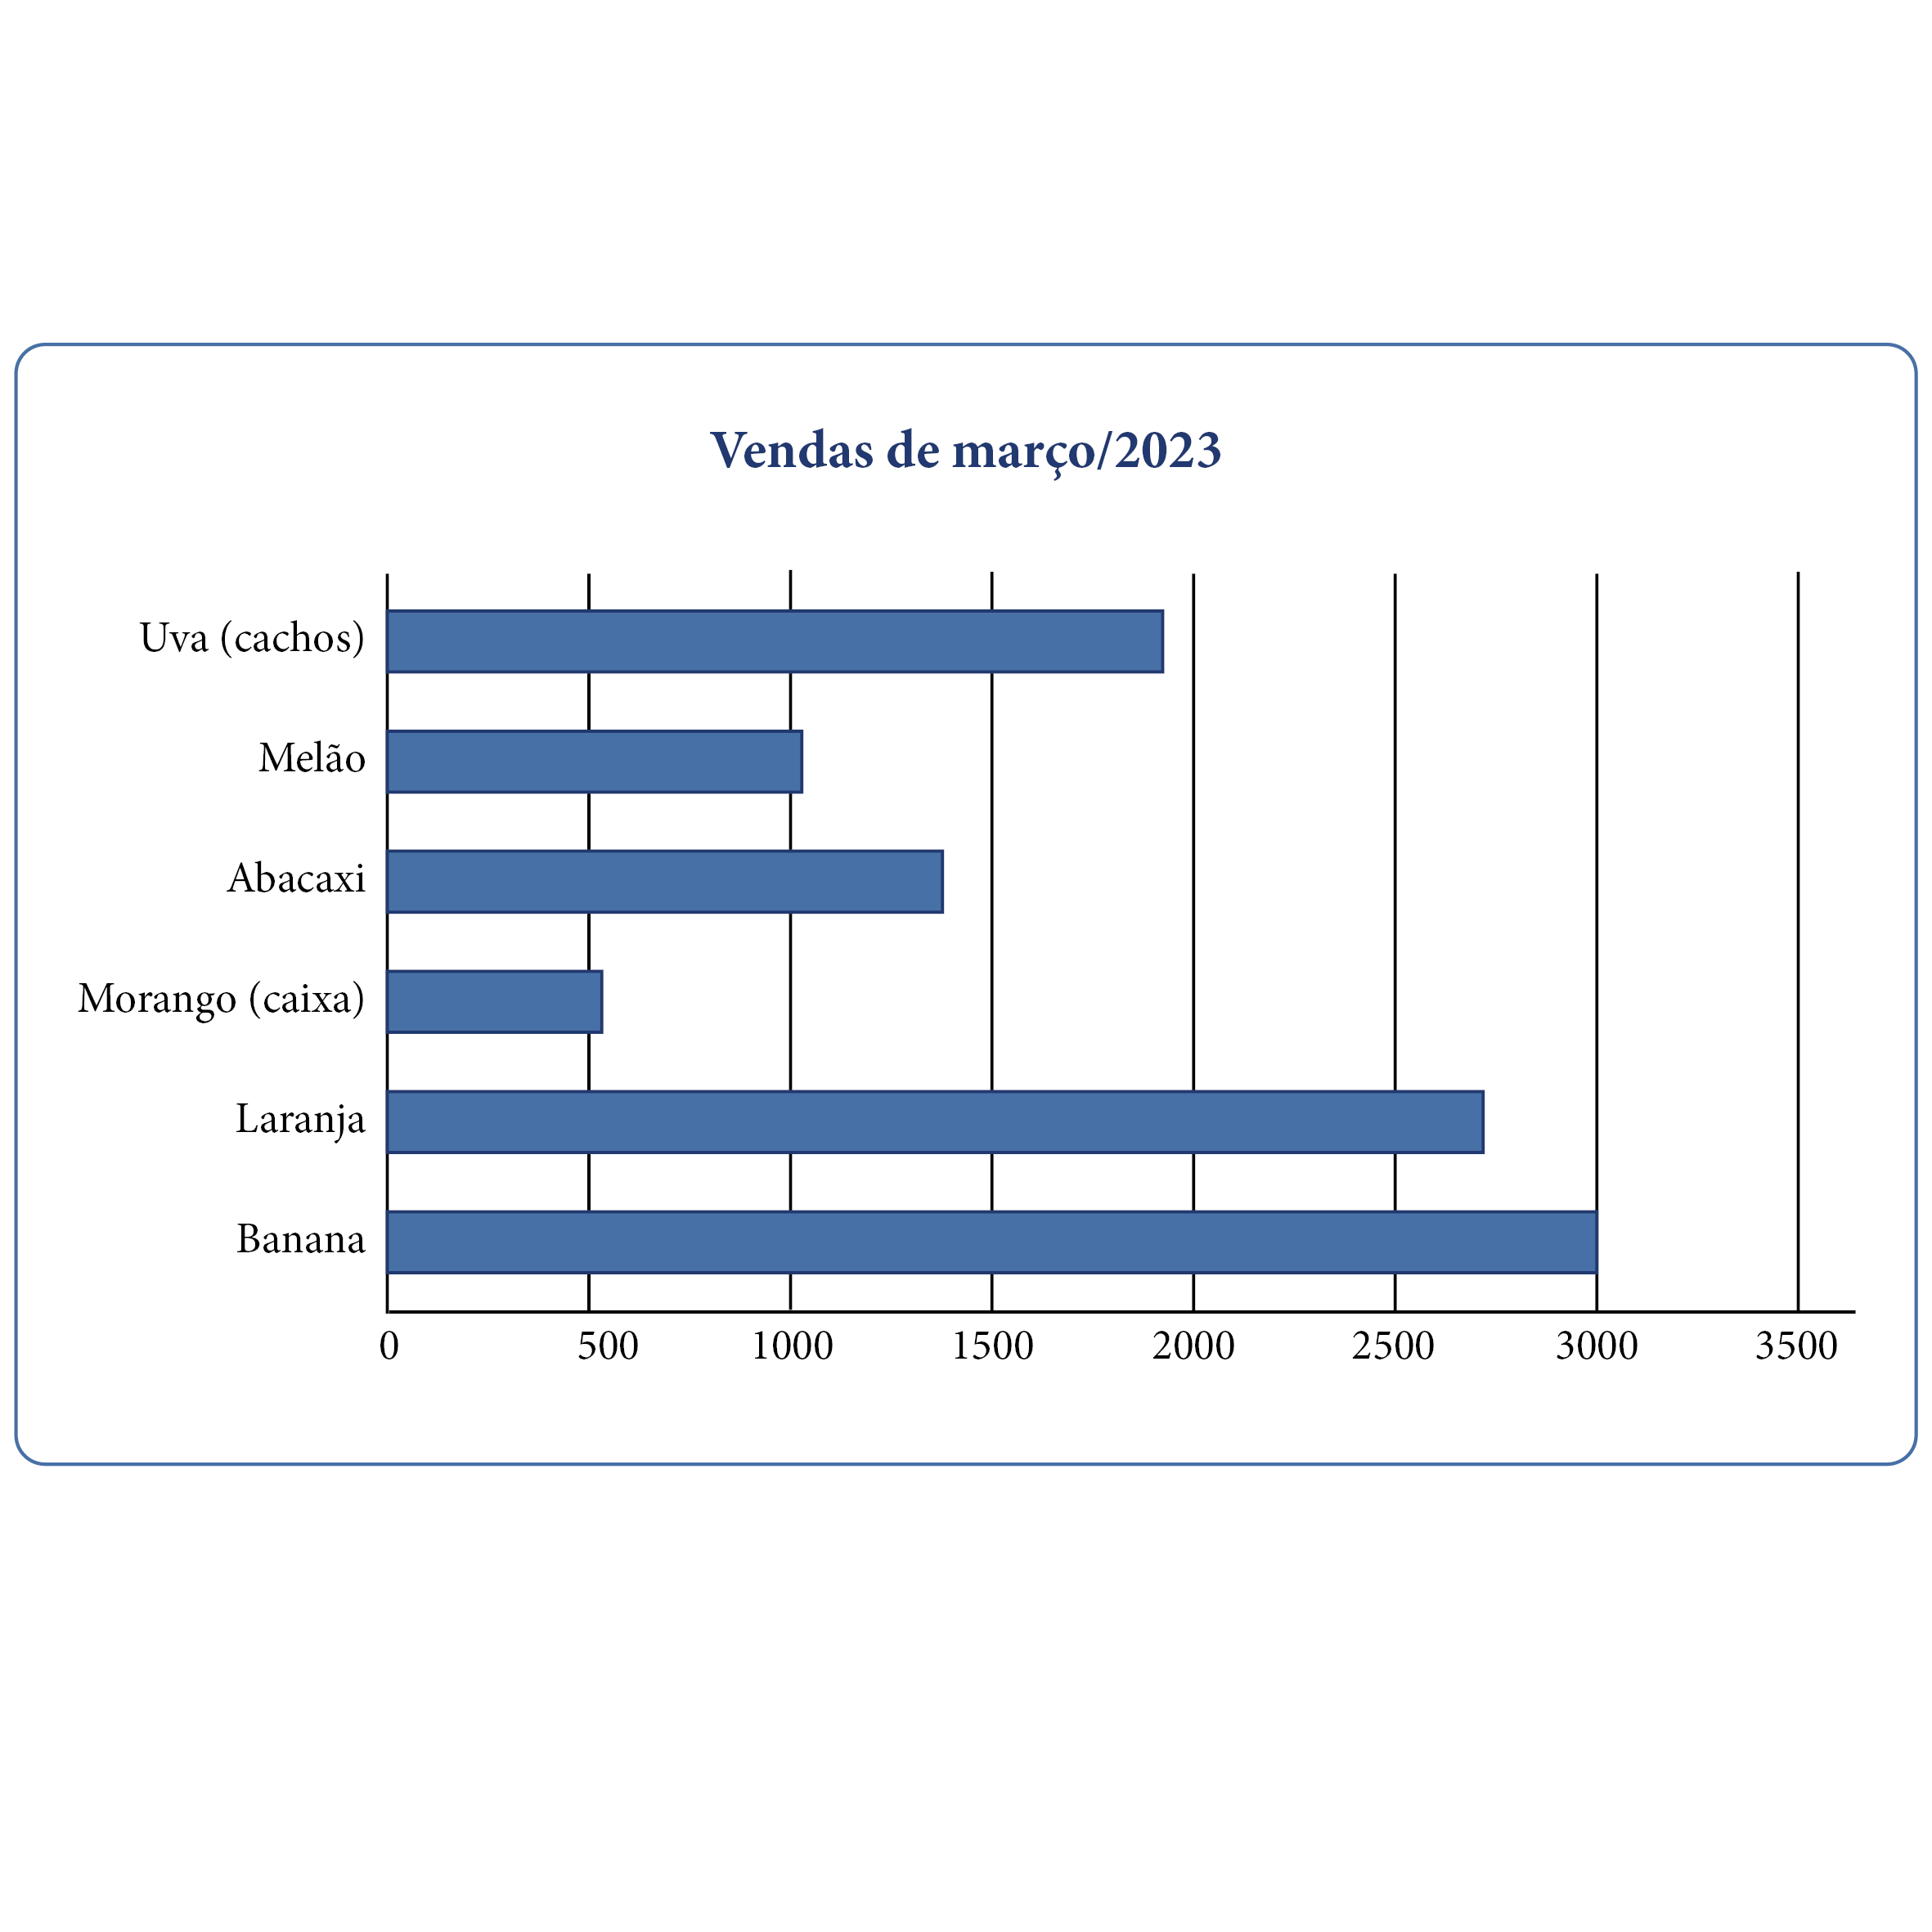
\includegraphics[width=.5\textwidth]{../ilustracoes/POR5/SAEB_5ANO_POR_FIGURA2.png}
\end{wrapfigure}

Cada barra representa a quantidade de uma fruta
vendida, e podemos comparar facilmente as quantidades. No gráfico de
barras (nesse caso, horizontais), as quantidades são representadas visualmente por barras que
crescem conforme o número representado aumenta. Assim, nesse gráfico, podemos
observar que a banana foi a fruta mais vendida no mês, enquanto a menos vendida foi o morango.

Gráficos e tabelas são muito importantes em muitas áreas, como na
ciência, na economia e até mesmo no esporte. Eles ajudam a nos comunicar
informações importantes de forma clara e fácil de entender.}

\pagebreak

\colorsec{Atividades}

\num{1} O que é um gráfico de barras?

\reduline{Trata-se de um gráfico que mostra quantidades diferentes de algo usando barras
verticais ou horizontais.\hfill}


\num{2} Para que serve um gráfico de barras?

\reduline{O gráfico de barras serve para comparar quantidades diferentes de algo.\hfill}

\num{3} O que é um gráfico de pizza?

\reduline{Trata-se de um gráfico que representa porcentagens de algo, usando fatias (porções) de uma uma figura parecida com uma pizza (o todo).\hfill}

\num{4} Para que serve um gráfico de pizza?

\reduline{O gráfico de pizza serve para mostrar a proporção de algo em relação ao todo.\hfill}

\num{5} Como podemos comparar quantidades usando um gráfico de barras?

\reduline{Por meio de um gráfico de barras, quantidades podem ser comparadas por meio da comparação entre as alturas (barras verticais) ou os comprimentos (barras horizontais) dos elementos do gráfico.}


Analise o gráfico a seguir para resolver as atividades de 6 a 8.

\begin{figure}[htpb!]
\centering
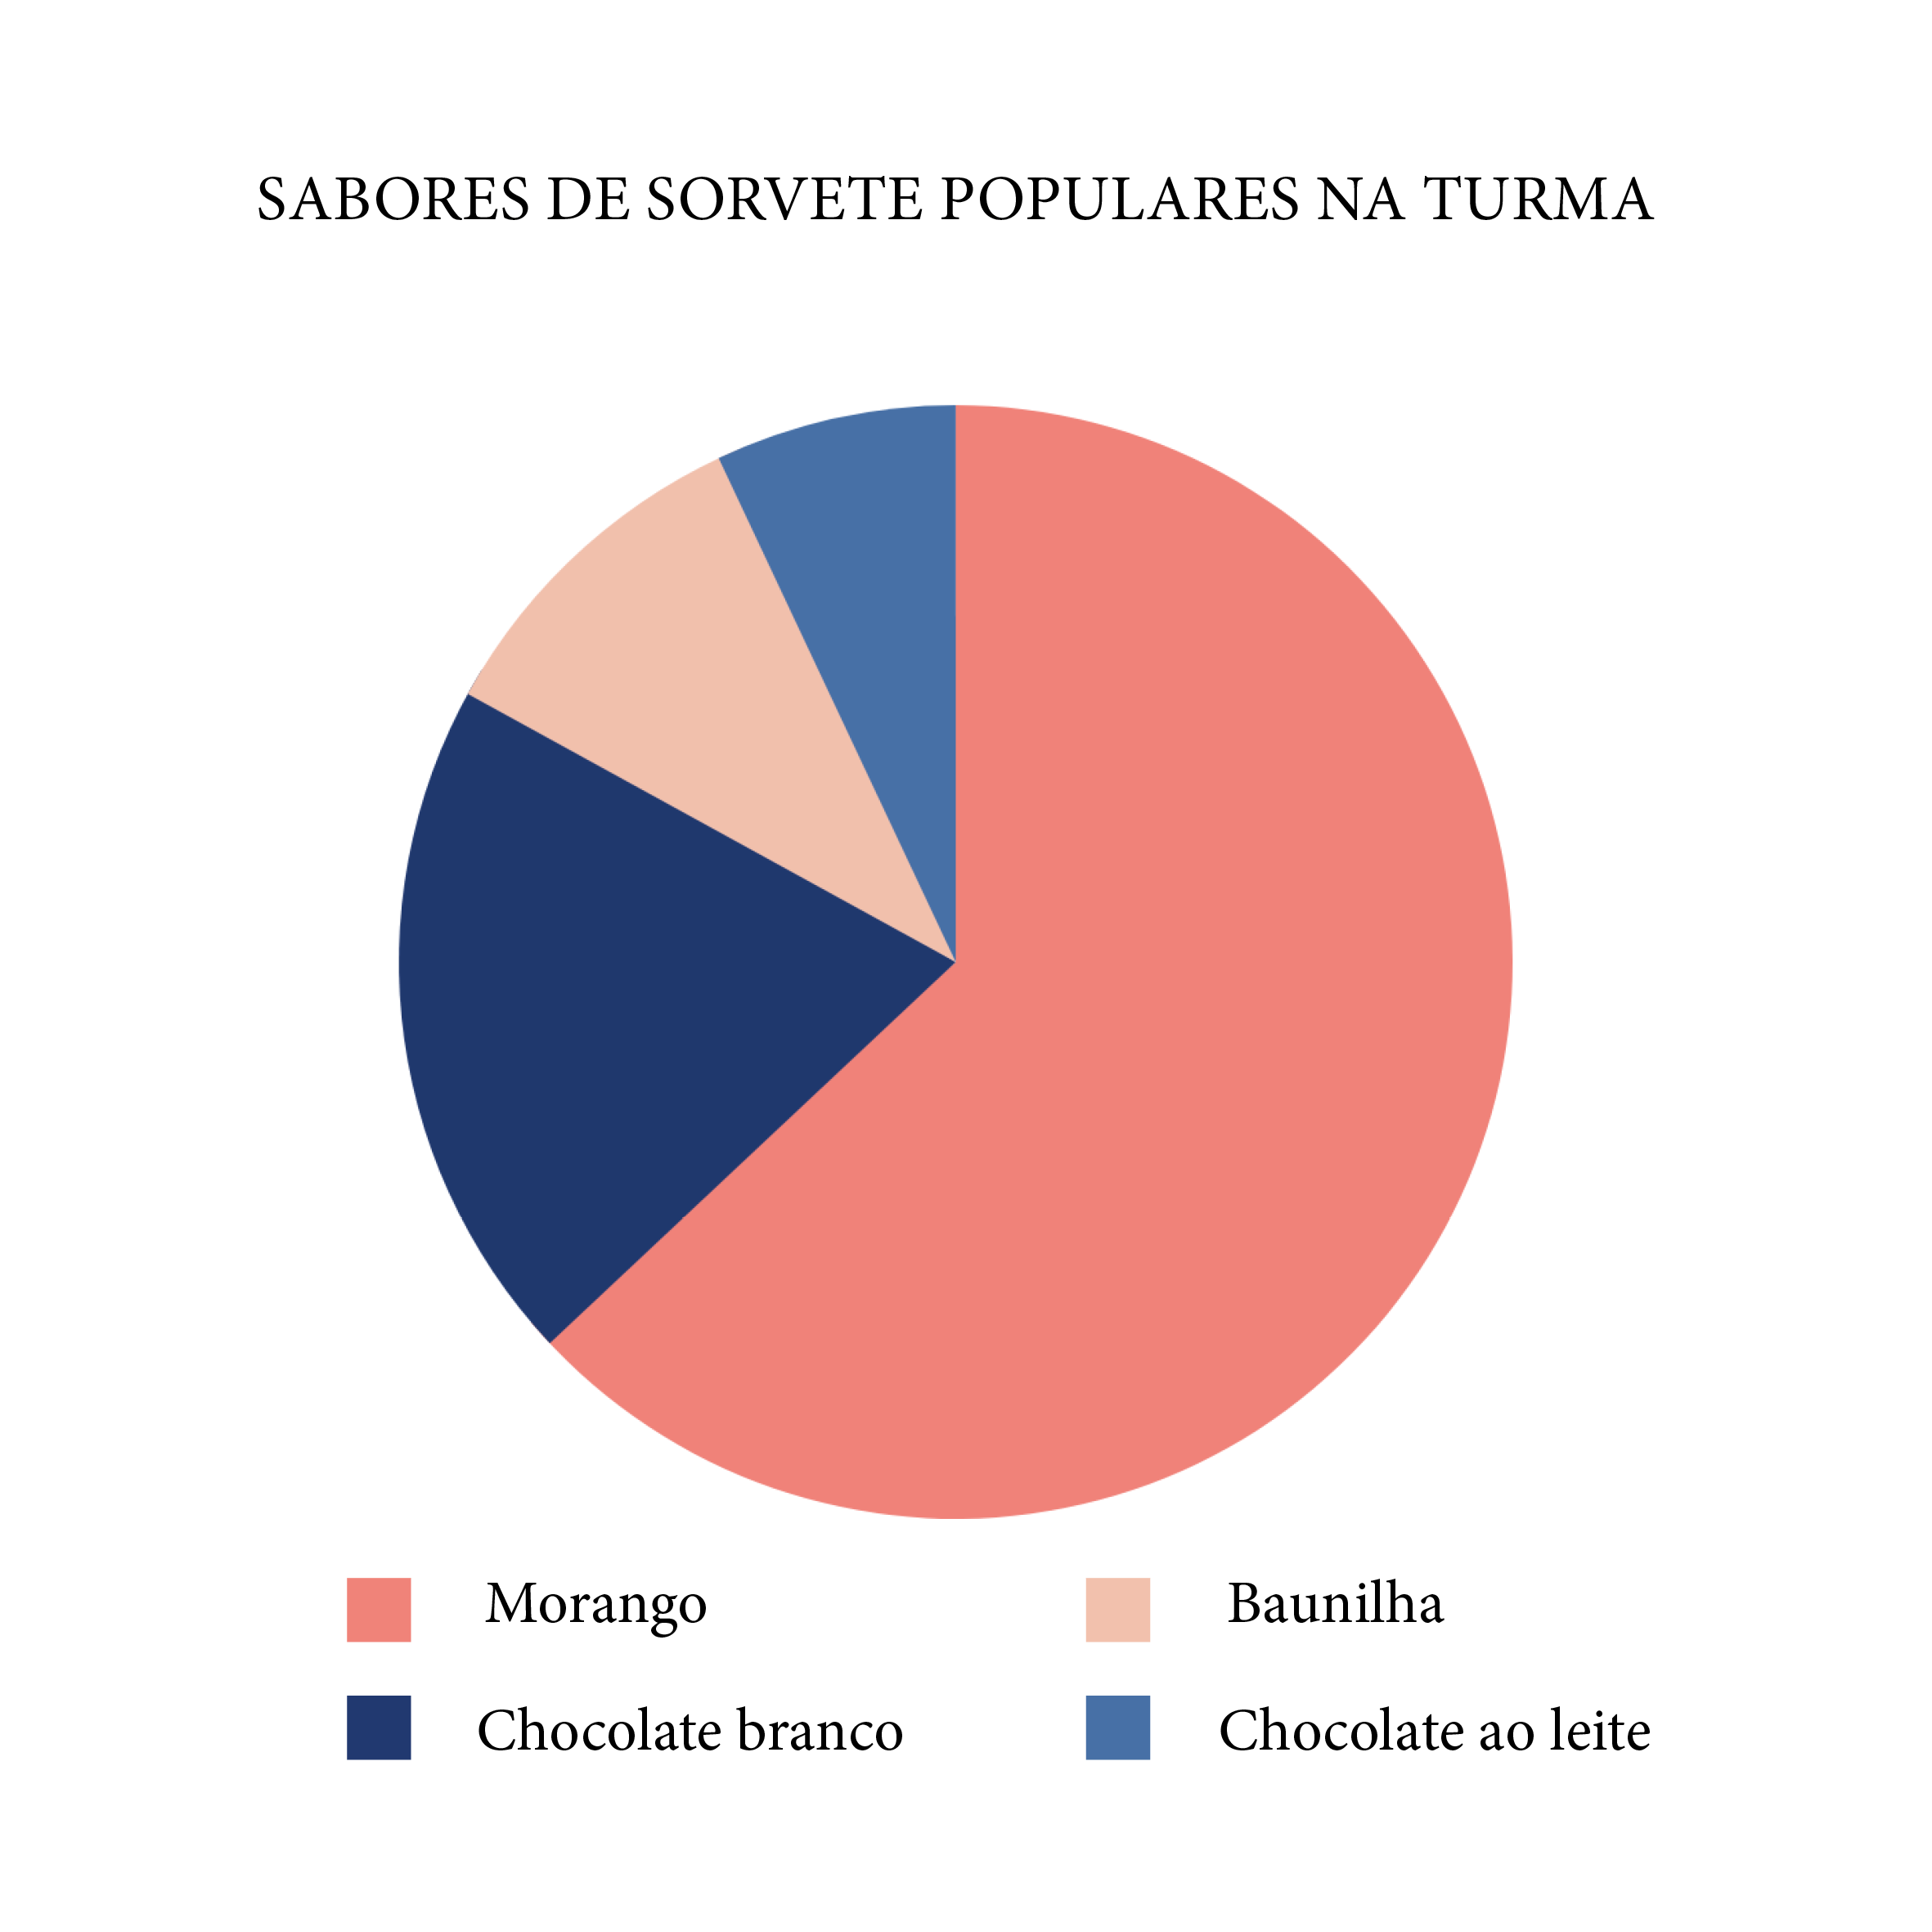
\includegraphics[width=.7\textwidth]{../ilustracoes/POR5/SAEB_5ANO_POR_FIGURA3.png}
\end{figure}

\num{6} Primeiro, faça o que se pede a seguir.

\begin{escolha}
\item Utilizando esse gráfico de pizza, como é possível saber qual é o sabor de sorvete mais popular na turma pesquisada?

\reduline{O sabor mais popular é aquele que é representado, no gráfico, pela fatia maior da pizza.\hfill}

\item Qual sabor de sorvete é mais popular na turma?

\reduline{O sorvete de morango.\hfill}

\item Qual sabor de sorvete é o menos popular na turma?

\reduline{O sorvete de chocolate ao leite.\hfill}
\end{escolha}

\num{7} Crie uma lista indicando, da menor proporção para a maior proporção, os sabores de sorvete que foram mencionados pelos membros da turma pesquisada.

\reduline{Chocolate ao leite < baunilha < chocolate branco < morango.\hfill}

\num{8} Com base nos dados do gráfico, adapte as informações para um gráfico de barras verticais.

\begin{mdframed}[linewidth=2pt,linecolor=salmao]
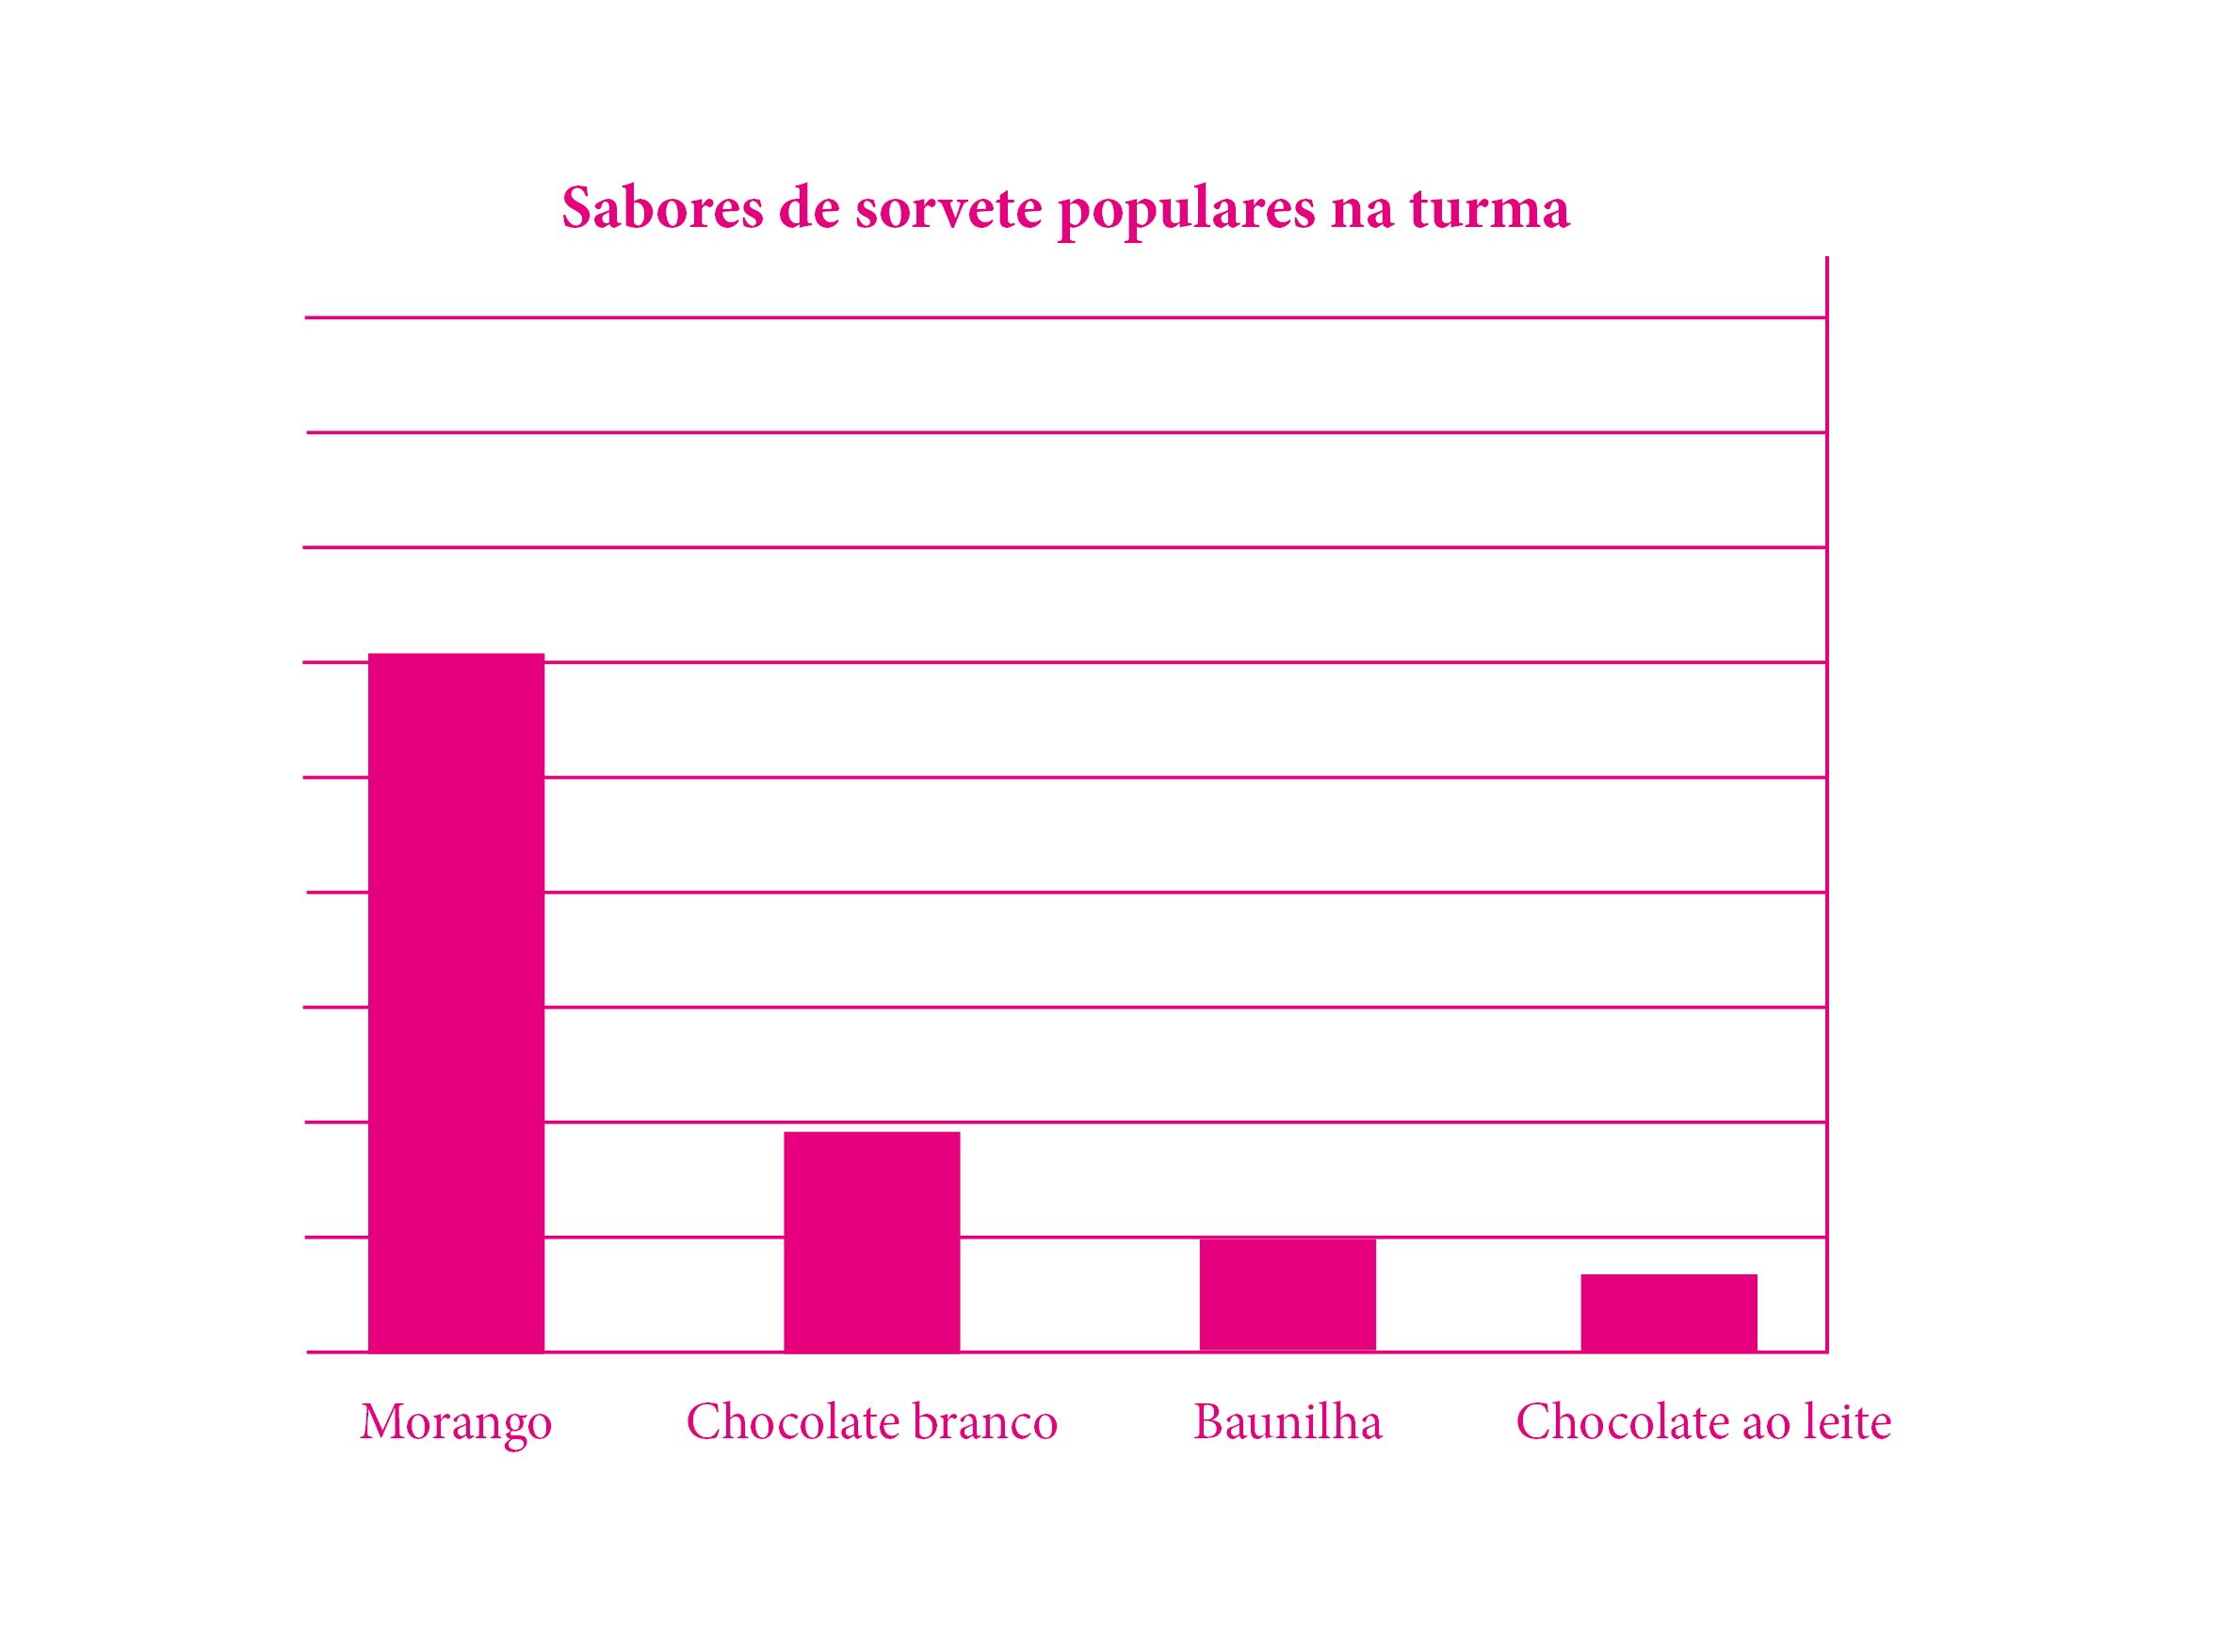
\includegraphics[width=\textwidth]{../ilustracoes/POR5/SAEB_5ANO_POR_FIGURA4.png}
\end{mdframed}


\num{9} A seguir, marque V para o que for verdadeiro e F para o que for falso.

\begin{boxlist}
\boxitem{F} Gráfico é uma forma escrita de organizar informações.

\boxitem{V} Pode ser mais fácil depreender determinados dados por meio de um gráfico.

\boxitem{V} Uma tabela e um gráfico podem estar vinculados no que se referem aos dados apresentados.

\boxitem{F} Uma tabela não pode originar um gráfico.

\boxitem{V} Um gráfico sem dados numéricos não pode ser adaptado para uma tabela.
\end{boxlist}

\num{10} Analise novamente este gráfico.

\begin{figure}[htpb!]
\centering
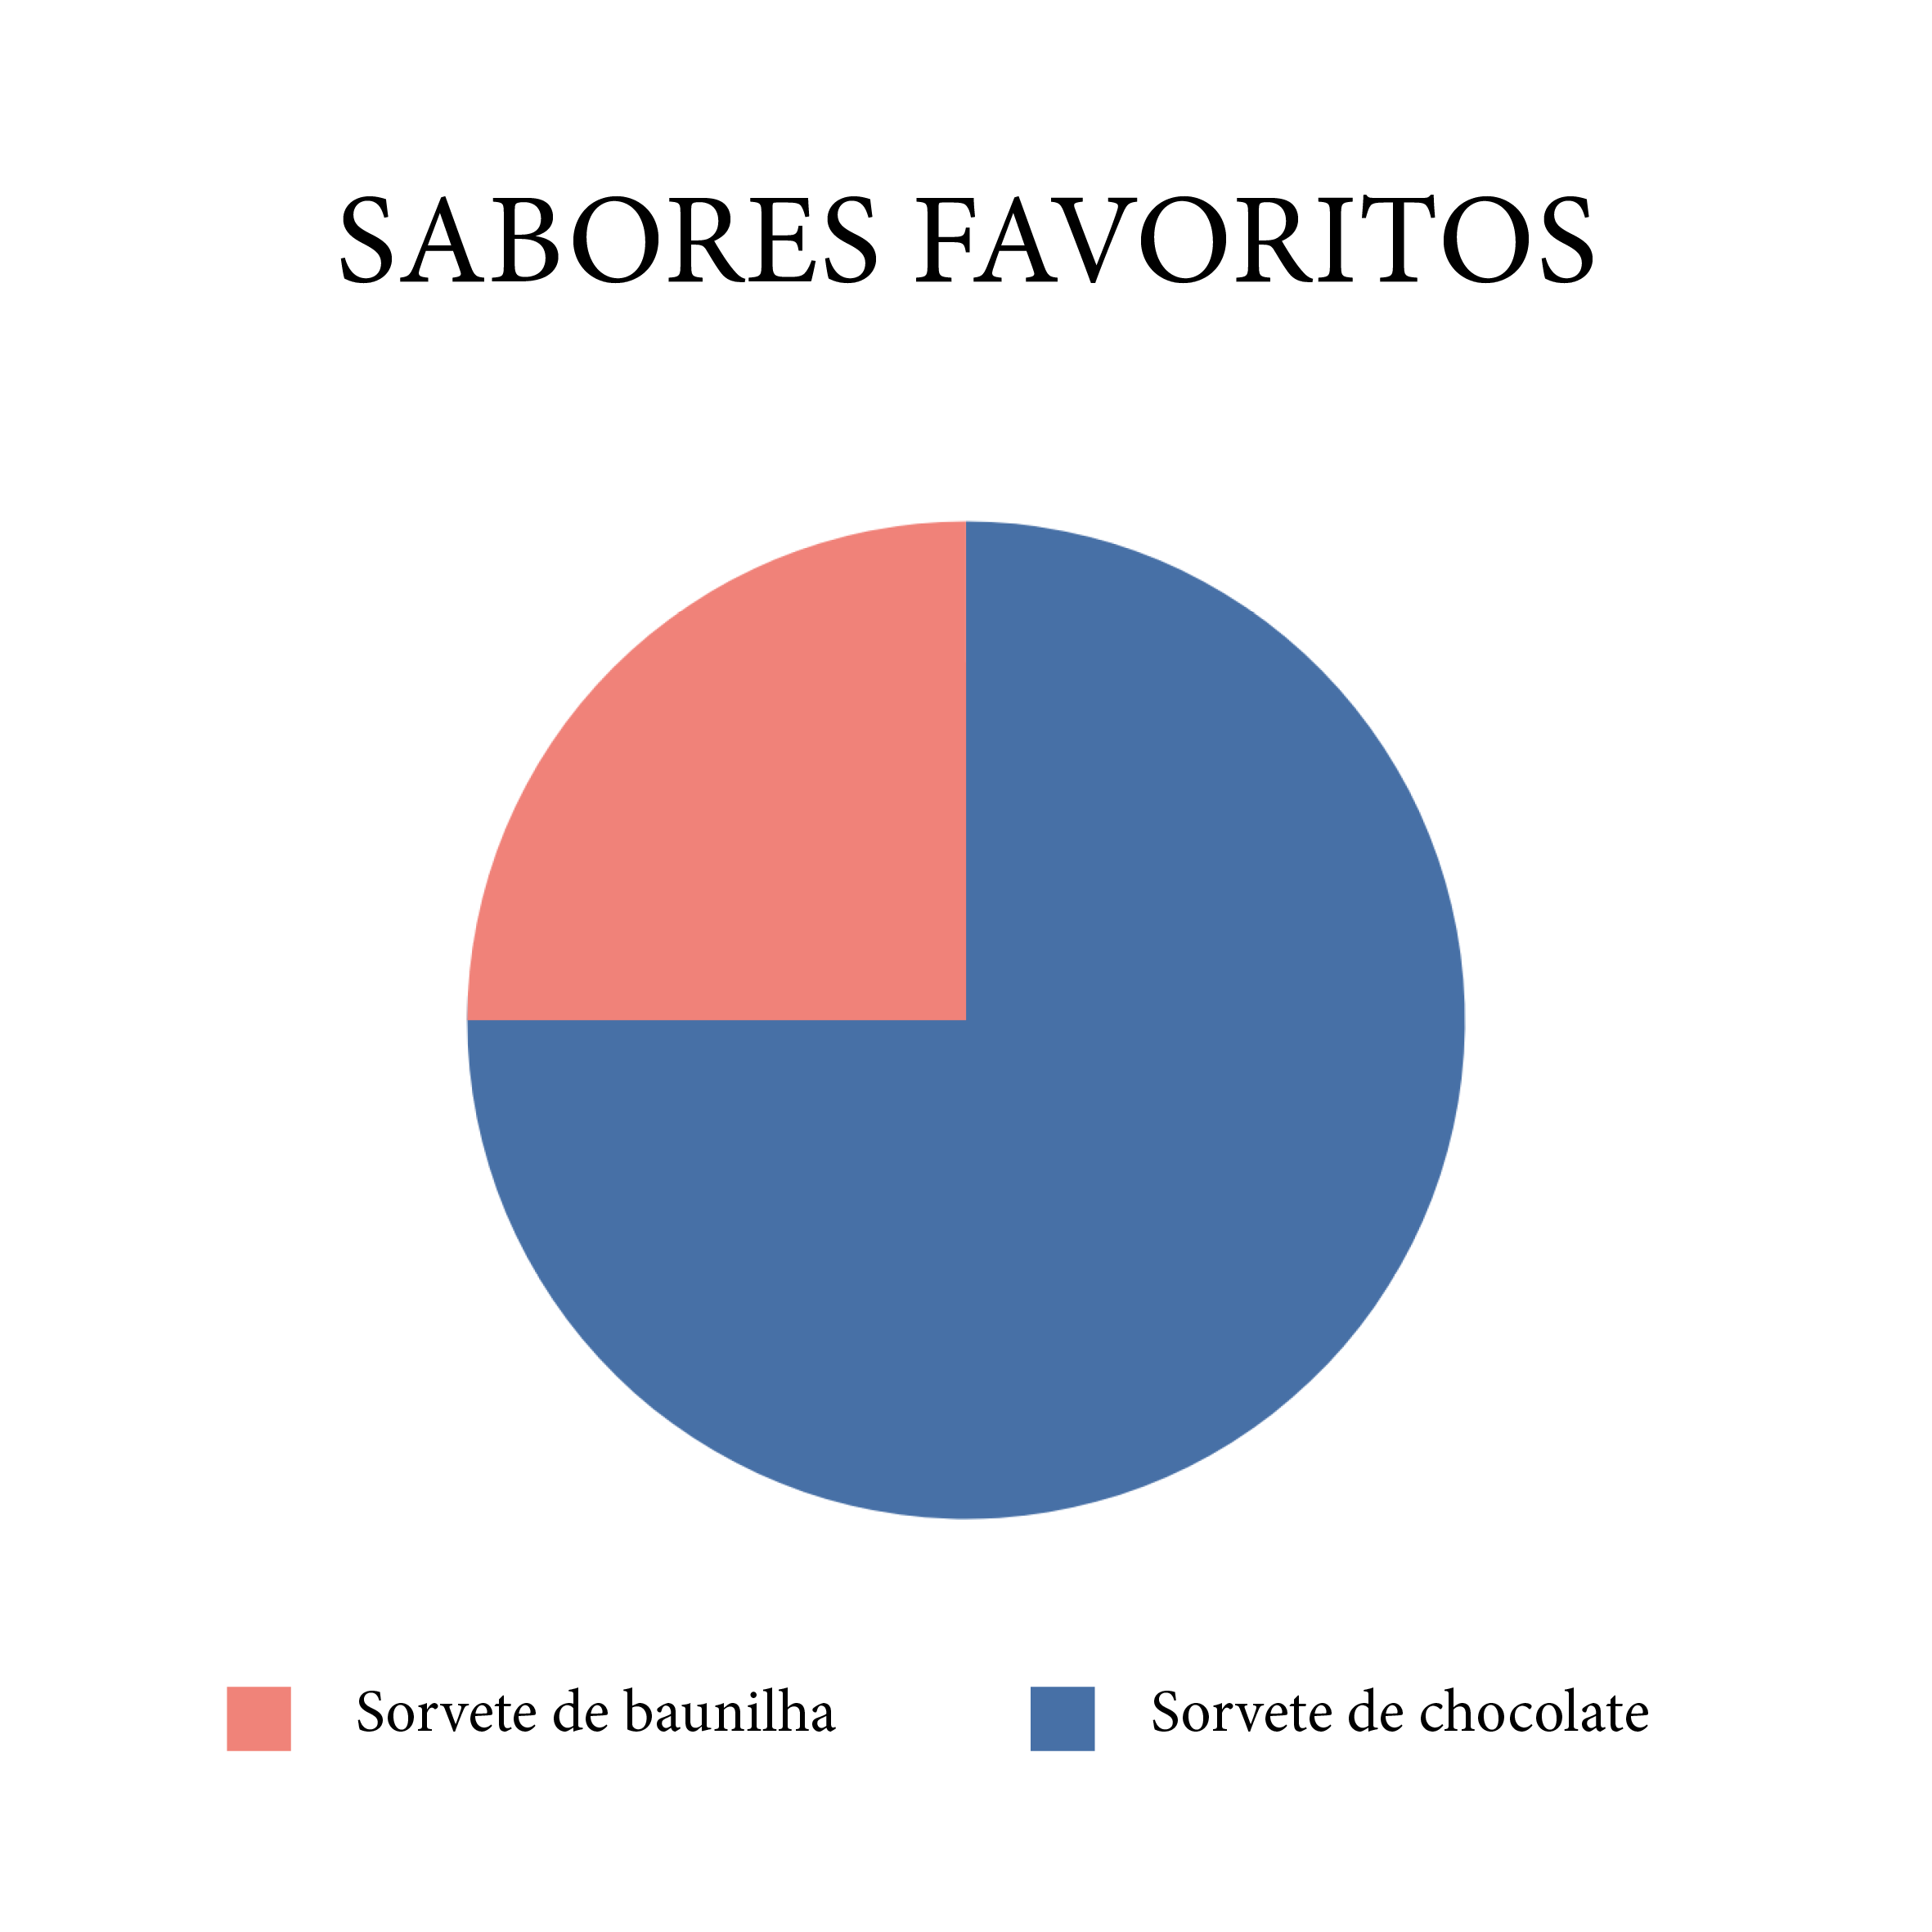
\includegraphics[width=.7\textwidth]{../ilustracoes/POR5/SAEB_5ANO_POR_FIGURA1.png}
\end{figure}

O número de pessoas que preferem sorvete de chocolate é menor ou maior que a metade do todo? Justifique sua resposta.

\reduline{O número de pessoas que preferem sorvete de chocolate é maior que a metade do todo, e isso pode ser afirmado porque a fatia da pizza que representa esse grupo é maior que meia pizza.\hfill}

\colorsec{Treino}

\noindent{} Analise o gráfico a seguir. Depois, responda às questões de 1 a 3.

\begin{figure}[htpb!]
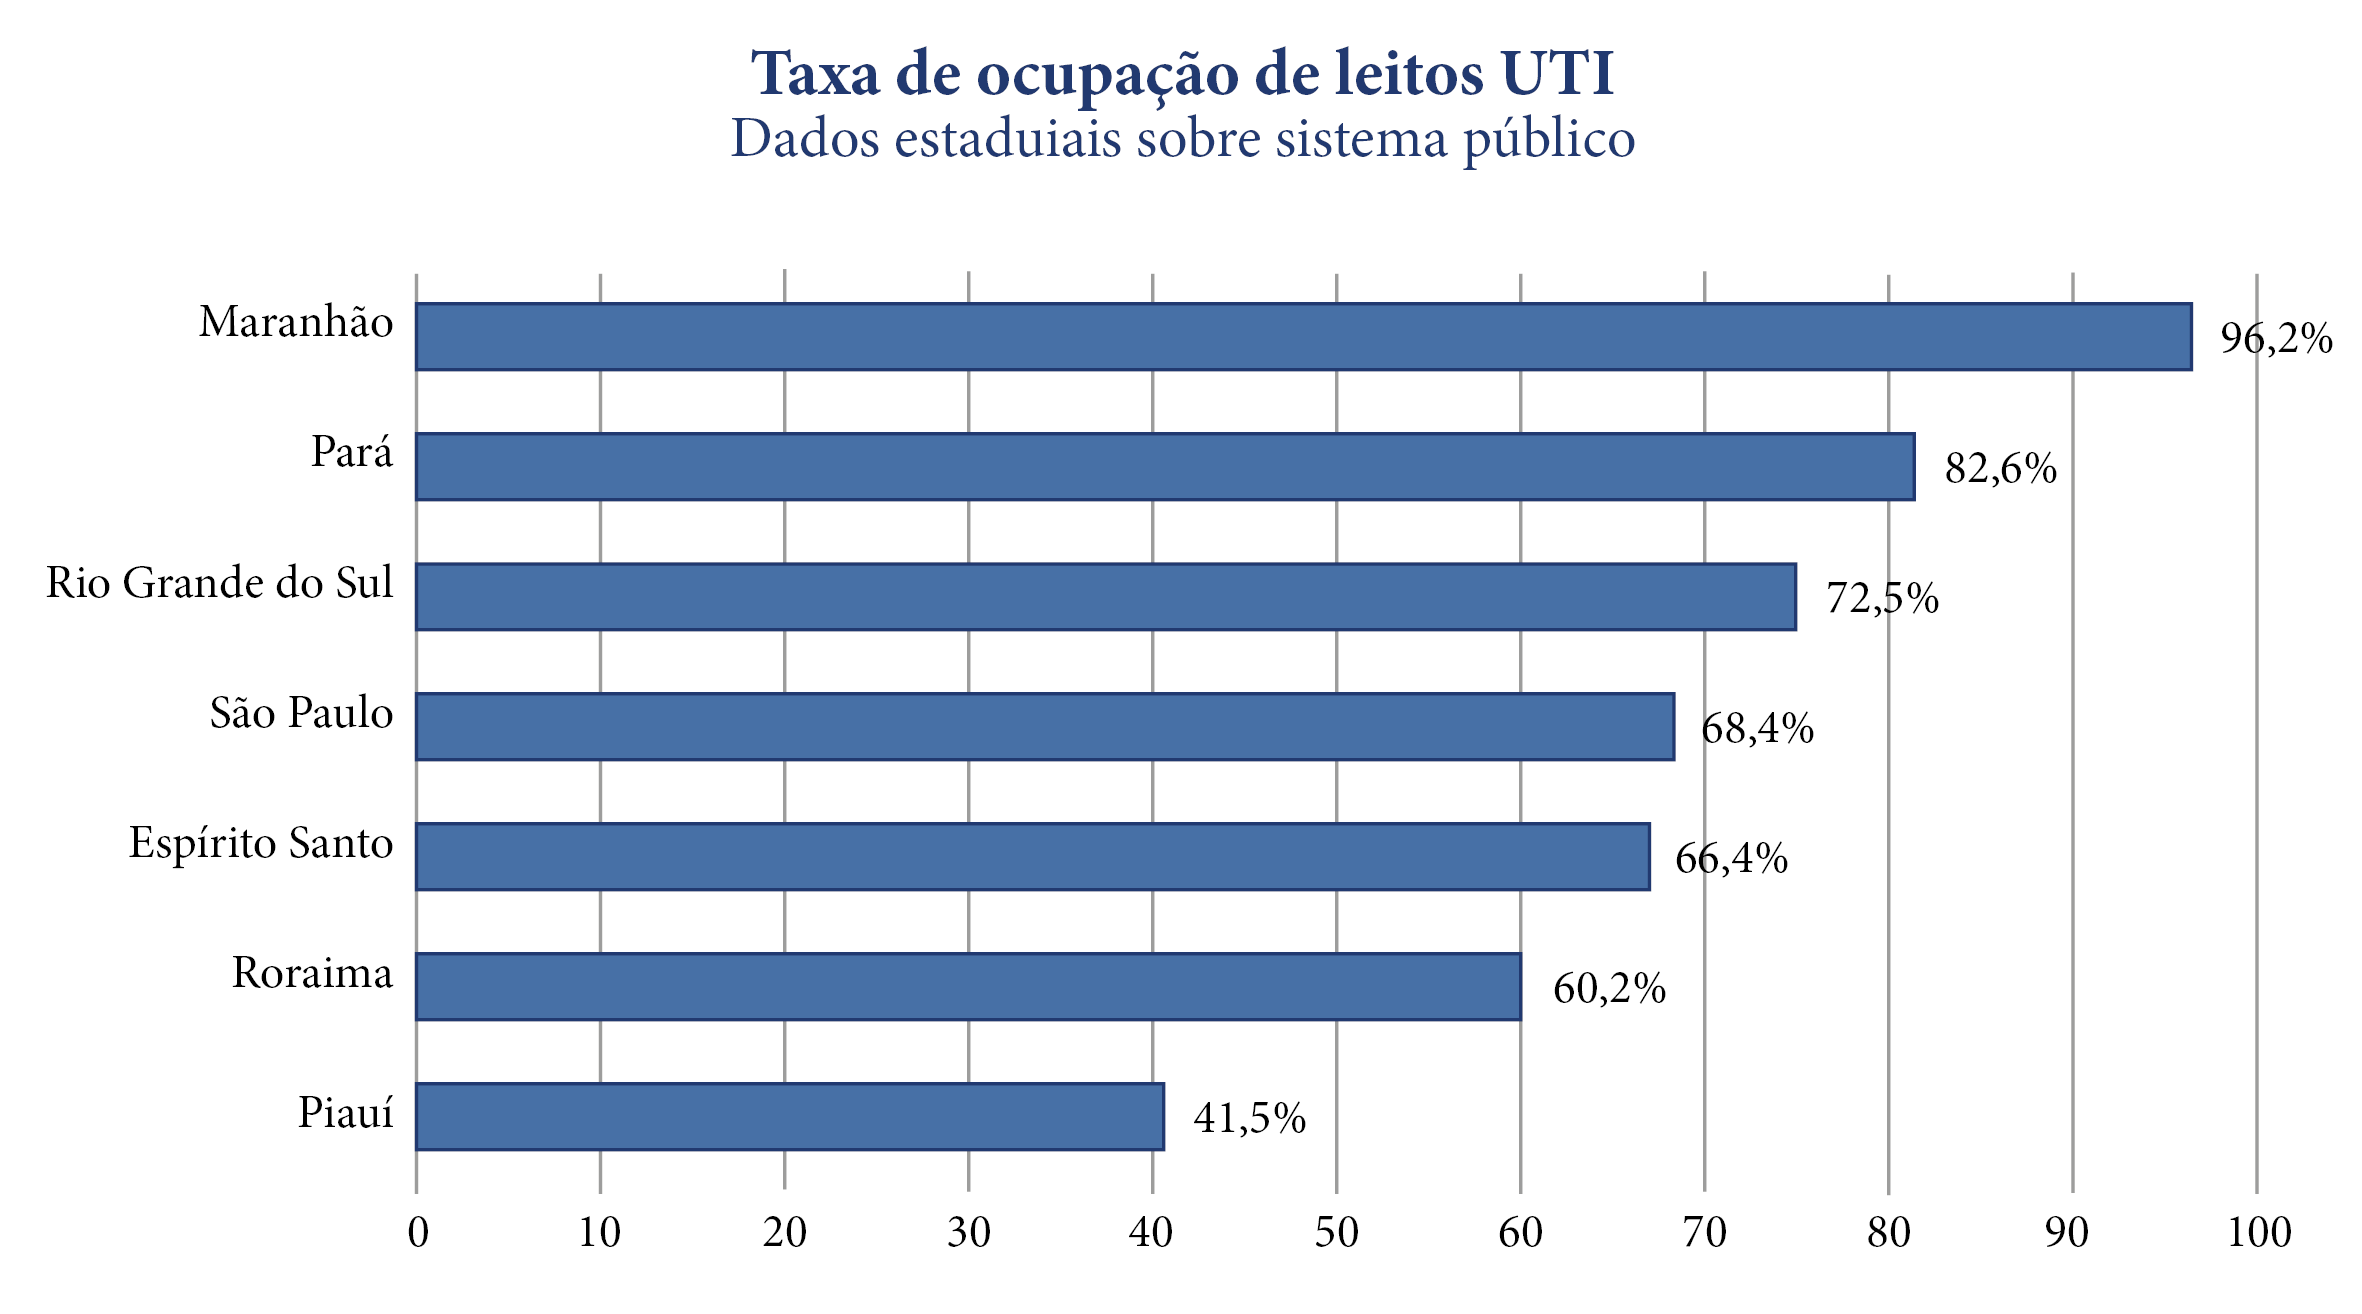
\includegraphics[width=\textwidth]{../ilustracoes/POR5/SAEB_5ANO_POR_FIGURA5.png}
\caption{Fonte de pesquisa: Matheus Magenta. BBC. Coronavírus: 10 gráficos para entender a situação atual do Brasil na pandemia. Disponível em: https://www.bbc.com/portuguese/brasil-52595760. Acesso em: 25 mar. 2023.}
\end{figure}

\num{1} Qual era a taxa de ocupação dos leitos de UTI para covid-19 no estado de São
Paulo em 10 de maio de 2020, de acordo com os dados apresentados?

\begin{minipage}{.5\textwidth}
\begin{escolha}
\item Cerca de 41\%.

\item Quase 100\%.

\item Perto de 69\%.

\item Mais de 80\%
\end{escolha}
\end{minipage}
\sidetext{SAEB: Analisar informações apresentadas em gráficos,
infográficos ou tabelas. Habilidades da BNCC: EF05LP23 -- Comparar
informações apresentadas em gráficos ou tabelas.}


\num{2} Que estados tinham mais próximas, segundo o gráfico, taxas de ocupação de leitor de UTI para covid-19?

\begin{minipage}{.5\textwidth}
\begin{escolha}
\item Maranhão e Pará.

\item Rio Grande do Sul e São Paulo.

\item São Paulo e Espírito Santo.

\item Piauí e Roraima.
\end{escolha}
\end{minipage}
\sidetext{SAEB: Analisar informações apresentadas em gráficos,
infográficos ou tabelas. Habilidades da BNCC: EF05LP23 -- Comparar
informações apresentadas em gráficos ou tabelas.}

\num{3} A partir da leitura do gráfico, indique qual foi o estado brasileiro que teve
maior taxa de ocupação de leitos na UTI.

\begin{minipage}{.5\textwidth}
\begin{escolha}
\item Pará.

\item Roraima.

\item São Paulo.

\item Maranhão.
\end{escolha}
\end{minipage}
\sidetext{SAEB: Analisar informações apresentadas em gráficos,
infográficos ou tabelas. Habilidades da BNCC: EF05LP23 -- Comparar
informações apresentadas em gráficos ou tabelas.}

\chapter{Passo a passo}
\markboth{Módulo 10}{}

\colorsec{Habilidades do SAEB}

\begin{itemize}
\item Identificar os mecanismos de progressão textual.

\item Identificar os mecanismos de referenciação lexical e pronominal.

\item Analisar relações de causa e consequência.
\end{itemize}

\marginnote{Os alunos serão apresentados ao tema da progressão textual, entendendo
que os textos são organizados em sequências, organizados tendo por base
nosso conhecimento de mundo e novas informações introduzidas pelo
próprio texto.\\
Habilidades da BNCC: EF05LP07, EF05LP27.}
\conteudo{
\begin{wrapfigure}{l}{.5\textwidth}
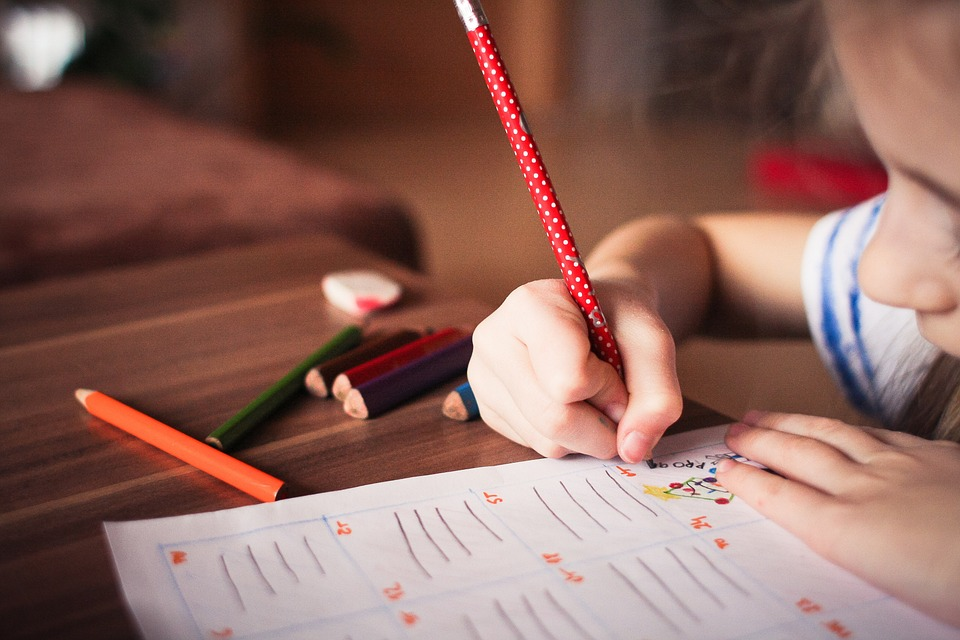
\includegraphics[width=.5\textwidth]{./imgs/img24.jpg}
%\caption{Fonte: https://pixabay.com/pt/photos/filho-crian\%c3\%a7a-jogar-estude-cor-865116/}
\end{wrapfigure}
Uma sequência de sons forma uma palavra. Palavras unidas de determinado modo formam uma frase e, no caso dos textos em prosa, frases organizam parágrafos, que são colocados em um texto como uma sequência lógica. A \textbf{progressão textual} é como uma estrada que nos leva de um lugar para outro: no caso dos textos, ela nos leva de uma ideia para outra.
Isso acontece porque os escritores usam palavras e frases para conectar
as ideias sobre as quais estão escrevendo. Por exemplo, eles podem usar palavras ou expressões
como “primeiro”, “em seguida” e “finalmente” para mostrar a ordem
do que está acontecendo. Isso denomina-se \textbf{sequenciação}.

Um tipo de relação que se pode construir por meio de uma sequenciação é a de \textbf{causa}, como neste exemplo:

\begin{itemize}
	\item Como você não aparecia, me cansei de esperar.
\end{itemize}

Observe que a causa de o enunciador ter se cansado de esperar é que a outra pessoa mencionada não aparecia. Podemos dizer que “Como você não aparecia” é a causa, enquanto “me cansei de esperar” é a \textbf{consequência} disso.

Outro ponto importante da construção de um texto é usar referências para
mencionar o que já foi dito ou anunciar o que será apresentado. Isso se dá por meio
da \textbf{referenciação}, que pode ser lexical ou pronominal. Suponha que você esteja escrevendo um
texto sobre um cachorro e, em vez de dizer “o cachorro” toda vez que
se referir a ele, você pode usar “ele” (um pronome que retoma e substitui “cachorro”) ou “o animal” (uma expressão que também retoma e substitui aquele substantivo).}


\colorsec{Atividades}

Leia o texto a seguir para entender os mecanismos de progressão textual.
Nesta pequena história, os mecanismos de progressão textual foram usados para
mostrar a ordem do que aconteceu.

\begin{quote}
\textbf{Um dia de passeio no parque}

Era uma vez uma menina chamada Sofia, que adorava passear no parque.
Certo dia, ela resolveu chamar sua melhor amiga, Ana, para
acompanhá-la em um delicioso piquenique.

Primeiro, elas foram ao supermercado comprar os alimentos que iriam
levar. Em seguida, caminharam até o parque, que ficava bem perto da casa
de Sofia. Chegando lá, encontraram um lugar muito bonito, com árvores,
flores e um lago com patinhos nadando.

Logo depois de estenderem a toalha no chão, começaram a comer e a
conversar. Ana contou sobre as férias que passou na praia e Sofia
falou sobre o livro que estava lendo.

Finalmente, quando já estava ficando tarde, elas recolheram a toalha e
os restos de comida e voltaram para casa, felizes e satisfeitas com o
passeio. Foi um dia muito agradável!

\fonte{Texto escrito para este material.}
\end{quote}


\num{1} Qual é o nome da menina que adorava passear no parque?

\reduline{Sofia.\hfill}


\num{2} O que Sofia resolveu fazer em certo dia?

\reduline{Ela resolveu chamar sua melhor amiga, Ana, para acompanhá-la em um delicioso piquenique.\hfill}
\linhas{2}

\num{3} O que as meninas fizeram primeiro?

\reduline{Elas foram ao supermercado comprar os alimentos que iriam levar.\hfill}
\linhas{1}

\num{4} Onde ficava o parque a que as meninas foram?

\reduline{O parque ficava bem perto da casa de Sofia.\hfill}
\linhas{1}


\num{5} O que as meninas encontraram quando chegaram ao parque?

\reduline{Elas encontraram um lugar muito bonito, com árvores, flores e um lago com patinhos nadando.\hfill}
\linhas{2}


\num{6} O que as meninas fizeram depois de estenderem a toalha no chão?

\reduline{Elas começaram a comer e a conversar.\hfill}
\linhas{1}


\num{7} Sobre o que Ana falou com Sofia?

\reduline{Ana contou sobre as férias que passou na praia.\hfill}
\linhas{1}


\num{8} Sobre o que Sofia falou com Ana?

\reduline{Sofia falou sobre o livro que estava lendo.\hfill}
\linhas{1}


\num{9} O que as meninas fizeram finalmente, quando já estava ficando tarde?

\reduline{Elas recolheram a toalha e os restos de comida e voltaram para casa.\hfill}
\linhas{2}


\num{10} Como as meninas se sentiram após o passeio?

\reduline{Elas se sentiram felizes e satisfeitas com o passeio.\hfill}
\linhas{1}


\colorsec{Treino}

Leia o texto a seguir para responder às questões de 1 a 3.

\begin{quote}
\textbf{O duende}

Era uma vez um pobre moleiro que mentiu ao rei, dizendo que sua filha
era capaz de transformar palha em ouro. O rei, que adorava ouro, ordenou
que a moça fosse trazida até ele para realizar o feito.

Assustada, a moça ficou presa em uma sala cheia de palha. Ela chorou,
sem saber o que fazer, até que apareceu um pequeno duende que se
ofereceu para transformar a palha em ouro em troca de algo. A moça
ofereceu seu colar, e o duende realizou o feito.

O rei ficou impressionado com a habilidade da moça e a levou para outra
sala cheia de palha, ordenando que ela transformasse em ouro novamente.
O duende apareceu novamente e, desta vez, pediu o anel da moça em troca
da transformação.

No terceiro dia, a moça foi levada para uma sala ainda maior e cheia de
palha. Ela não tinha mais nada para oferecer ao duende; então ele
sugeriu que ela desse a ele seu primeiro filho quando nascesse. Sem
escolha, a moça aceitou. O rei ficou ainda mais impressionado e decidiu
se casar com a jovem.

Anos depois, a moça deu à luz uma criança, porém o duende retornou para
pegá-la. A agora rainha implorou por sua liberdade e ofereceu tudo o que
tinha para mantê-lo longe do bebê. O duende sugeriu que, se ela
conseguisse adivinhar seu nome, ele desistiria de seu objetivo.

Assim, a rainha enviou mensageiros por todo o mundo, para descobrir o
nome do duende, mas não teve sucesso. Um dia, andando pela floresta, a
rainha ouviu o duende cantando seu próprio nome, Rumpelstiltskin. Assim,
revelando saber o nome do duende, a rainha pôde manter seu bebê e viver
feliz para sempre.

\fonte{Fonte de pesquisa: Irmãos Grimm. Rumpelstilzinho. Disponível em:
\emph{https://www.grimmstories.com/pt/grimm\_contos/o\_anao\_saltador}.
Acesso em: 27 mar. 2023.}
\end{quote}

\num{1} Qual foi a primeira consequência da mentira contada pelo moleiro ao rei?

\begin{escolha}
\item A filha do moleiro teve de transformar palha em ouro para o rei.

\item O rei decidiu se casar com a filha do moleiro.

\item O duende apareceu para ajudar a filha do moleiro em troca de algo.

\item A filha do moleiro teve de entregar seu primeiro filho para o duende quando nascesse.
\end{escolha}

\coment{Habilidades do SAEB: Analisar relações de causa e consequência. BNCC:
EF35LP26 -- Ler e compreender, com certa autonomia, narrativas ficcionais que apresentem
cenários e personagens, observando os elementos da estrutura narrativa: enredo, tempo, espaço,
personagens, narrador e a construção do discurso indireto e discurso direto.}


\num{2} Releia este trecho do texto.

\begin{quote}
Ela chorou, sem saber o que fazer, até que apareceu um pequeno duende que se
ofereceu para transformar a palha em ouro em troca de algo. A moça
ofereceu seu colar, e o duende realizou o feito.
\end{quote}

Uma palavra ou uma expressão que, nesse trecho, cria uma referência temporal é

\begin{minipage}{.5\textwidth}
\begin{escolha}
\item “sem”.

\item “até que”.

\item “para”.

\item “e”.
\end{escolha}
\end{minipage}
\sidetext{Identificar os mecanismos de progressão textual. BNCC:
EF05LP07 -- Identificar, em textos, o uso de conjunções e a relação
que estabelecem entre partes do texto: adição, oposição, tempo, causa,
condição, finalidade.}


\num{3} Releia este trecho do texto.

\begin{quote}
Anos depois, a moça deu à luz uma criança, porém o duende retornou para
pegá-la. A agora rainha implorou por sua liberdade e ofereceu tudo o que
tinha para mantê-lo longe do bebê. O duende sugeriu que, se ela
conseguisse adivinhar seu nome, ele desistiria de seu objetivo.
\end{quote}

Assinale uma análise correta sobre o uso de pronomes nesse trecho

\begin{escolha}
\item O “o” que antecede “duende”, em “porém o duente retornou” é um pronome que antecipa a palavra que acompanha.

\item O pronome “a”, em “pegá-la”, retoma e substitui o filho da moça, que apareceu como “uma criança”.

\item O pronome “sua”, ligado a “liberdade”, refere-se ao duende, que apareceu na frase anterior.

\item O pronome “seu”, ligado a “nome”, refere-se à moça que então era rainha.
\end{escolha}

\coment{Identificar os mecanismos de referenciação lexical e pronominal.}





